% !TeX program = xelatex
% !TeX encoding = UTF-8 Unicode
\documentclass[12pt,a4paper]{report}

\usepackage[a4paper,margin=2.5cm]{geometry}
\usepackage{fontspec}
\usepackage{graphicx}
\usepackage{amsmath}
\usepackage{array}
\usepackage{booktabs}
\usepackage{longtable}
\usepackage{tabularx}
\usepackage{float}
\usepackage{enumitem}
\usepackage{hyperref}
\usepackage{fancyhdr}
\usepackage{setspace}
\usepackage{indentfirst}
\usepackage{tikz}
\usepackage[american]{circuitikz}
\usepackage{xcolor}
\usepackage{listings}

\usetikzlibrary{chains,positioning,shapes.geometric}

\renewcommand{\contentsname}{Mục lục}
\renewcommand{\listfigurename}{Danh sách hình ảnh}

\setmainfont{Times New Roman}
\setsansfont{Arial}
\setmonofont{Courier New}

\hypersetup{
  colorlinks=true,
  linkcolor=black,
  urlcolor=black,
  pdftitle={Bao cao he thong CAN tren ESP32},
  pdfauthor={Can bo sung thong tin sinh vien},
  pdfsubject={CAN Bus, ESP32, IDS, Automotive Security}
}

\onehalfspacing
\setlength{\parindent}{1.2cm}
\setlength{\parskip}{0.4em}
\setlength{\headheight}{16pt}
\sloppy

\pagestyle{fancy}
\fancyhf{}
\fancyhead[L]{Báo cáo kỹ thuật hệ thống CAN trên ESP32}
\fancyhead[R]{\thepage}

\newcommand{\reportsection}[1]{%
  \section*{#1}%
  \addcontentsline{toc}{section}{#1}%
}

\newcommand{\reportsubsection}[1]{%
  \subsection*{#1}%
  \addcontentsline{toc}{subsection}{#1}%
}

\newcommand{\placeholderfigure}[2]{%
  \begin{figure}[H]
    \centering
    \fbox{%
      \parbox{0.82\textwidth}{%
        \centering
        \vspace{1.2cm}
        #1\\
        Bổ sung hình minh họa sau.
        \vspace{1.2cm}
      }%
    }
    \caption{#2}
  \end{figure}
}

\newcommand{\missingnote}[1]{%
  \begin{quote}
    \textbf{Ghi chú:} #1
  \end{quote}
}

\lstset{
  basicstyle=\ttfamily\small,
  breaklines=true,
  columns=fullflexible,
  keepspaces=true,
  showstringspaces=false
}

\begin{document}

\begin{titlepage}
  \thispagestyle{empty}
  \begin{tikzpicture}[remember picture, overlay]
    \draw[blue!70!violet, line width=2.4pt]
      ($(current page.north west)+(0.78cm,-0.78cm)$)
      rectangle
      ($(current page.south east)+(-0.78cm,0.78cm)$);
    \draw[blue!45!violet, line width=0.9pt]
      ($(current page.north west)+(1.03cm,-1.03cm)$)
      rectangle
      ($(current page.south east)+(-1.03cm,1.03cm)$);

    \node[
      align=center,
      text width=0.82\paperwidth,
      font=\bfseries\fontsize{18}{23}\selectfont
    ] at ($(current page.north)+(0,-3.25cm)$) {ĐẠI HỌC QUỐC GIA HÀ NỘI};

    \node[
      align=center,
      text width=0.82\paperwidth,
      font=\bfseries\fontsize{18}{23}\selectfont
    ] at ($(current page.north)+(0,-4.25cm)$) {TRƯỜNG ĐẠI HỌC CÔNG NGHỆ};

    \IfFileExists{images/cover-logo.png}{%
      \node at ($(current page.north)+(0,-7.05cm)$) {%
        
\includegraphics[width=4.1cm]{images/cover-logo.png}%
      };
    }{}

    \node[
      align=center,
      text width=0.78\paperwidth,
      font=\bfseries\fontsize{18}{23}\selectfont
    ] at ($(current page.north)+(0,-11.55cm)$) {%
      CyberCAN Defense: Phát hiện và phòng\\
      thủ xâm nhập mạng nội bộ ô tô%
    };

    \node[
      align=center,
      font=\fontsize{14}{18}\selectfont
    ] at ($(current page.north)+(0,-14.45cm)$) {Nhóm 4};

    \node at ($(current page.north)+(0,-19.1cm)$) {%
      \fontsize{12}{16}\selectfont
      \begin{tabular}{@{}p{5.4cm}r@{}}
        Phạm Thế Duy & 23021787 \\
        Bùi Đăng Dương & 23020795 \\
        Nguyễn Thị Ngọc Bích & 23021770 \\
        Nguyễn Hữu Thái Dương & 23021789 \\
      \end{tabular}
    };

    \node[
      align=center,
      text width=0.72\paperwidth,
      font=\fontsize{13}{18}\selectfont
    ] at ($(current page.north)+(0,-23.0cm)$) {%
      Cơ sở đo lường và điều khiển số\\[0.38cm]
      Lớp: ELT3207 1\\[0.38cm]
      Giảng viên: TS. Hoàng Gia Hưng\\[0.38cm]
      Mentor: Nguyễn Quang Khôi%
    };

    \node[
      align=center,
      font=\bfseries\fontsize{14}{18}\selectfont
    ] at ($(current page.south)+(0,1.65cm)$) {Hà Nội, Tháng 6 năm 2026};
  \end{tikzpicture}
  \null
\end{titlepage}



\pagenumbering{roman}
\chapter*{Lời cam đoan}
\addcontentsline{toc}{chapter}{Lời cam đoan}

Chúng em cam đoan báo cáo ``Hệ thống giám sát, phát hiện và phòng thủ xâm nhập CAN bus trên nền tảng ESP32'' là kết quả học tập và nghiên cứu do chính nhóm thực hiện dưới sự hướng dẫn của giảng viên phụ trách học phần và các cá nhân hỗ trợ chuyên môn nếu có. Nội dung trình bày trong báo cáo được xây dựng trên cơ sở khảo sát tài liệu, phân tích mã nguồn, triển khai mô hình thực nghiệm và tổng hợp kết quả theo phạm vi mà nhóm đã thực hiện.

Nhóm cũng cam đoan các thông tin, hình ảnh, nhận xét và kết quả được nêu trong báo cáo là trung thực, phản ánh đúng quá trình thực hiện tại thời điểm biên soạn. Những nội dung tham khảo từ tài liệu, bài báo, báo cáo hoặc nguồn kỹ thuật khác đều cần được trích dẫn và ghi nhận phù hợp trong phần tài liệu tham khảo của báo cáo.

Nếu có sai sót liên quan đến tính trung thực học thuật, nguồn gốc nội dung hoặc việc sử dụng tài liệu tham khảo, chúng em xin chịu trách nhiệm trước giảng viên và quy định của học phần.

\clearpage
\chapter*{Lời cảm ơn}
\addcontentsline{toc}{chapter}{Lời cảm ơn}

Trong quá trình thực hiện báo cáo và phát triển mô hình thực nghiệm về an ninh mạng CAN, nhóm đã nhận được nhiều sự hướng dẫn và hỗ trợ quý báu từ giảng viên, bạn học và những người đồng hành trong quá trình học tập. Chúng em xin bày tỏ sự biết ơn chân thành tới giảng viên phụ trách học phần vì đã định hướng đề tài, góp ý về nội dung chuyên môn và hỗ trợ nhóm trong quá trình hoàn thiện báo cáo.

Nhóm cũng xin cảm ơn các cá nhân và tập thể đã hỗ trợ về tài liệu kỹ thuật, thiết bị thực nghiệm, môi trường phát triển và những trao đổi chuyên môn liên quan đến hệ thống CAN, ESP32 cũng như các khía cạnh an ninh mạng nội bộ ô tô. Những góp ý đó đã giúp nhóm từng bước hoàn thiện mô hình, cải thiện cách trình bày và hiểu rõ hơn ý nghĩa thực tiễn của đề tài.

Do giới hạn về thời gian, phạm vi học phần và điều kiện thử nghiệm, báo cáo khó tránh khỏi những thiếu sót nhất định. Chúng em rất mong tiếp tục nhận được các ý kiến nhận xét và góp ý để hoàn thiện hơn nội dung nghiên cứu cũng như rút kinh nghiệm cho các công việc học thuật và kỹ thuật sau này.

\clearpage
\tableofcontents
\clearpage
\addcontentsline{toc}{chapter}{Danh sách hình ảnh}
\listoffigures
\clearpage
\chapter*{Danh sách liên kết}
\addcontentsline{toc}{chapter}{Danh sách liên kết}

\begin{itemize}[leftmargin=*]
    \item \href{https://github.com/vnulic/CAN-ESP32.git}{\textcolor{blue}{Github}}
    \item \href{https://drive.google.com/drive/folders/1q_ydLcVppM0UkqJ5nY256r0bSRisEmvg}{\textcolor{blue}{Thư mục video minh họa các kịch bản tấn công và phòng thủ DoS, Replay, Fuzzing, Spoofing}}
\end{itemize}

\clearpage

\pagenumbering{arabic}

\chapter*{Lời mở đầu}
\addcontentsline{toc}{chapter}{Lời mở đầu}

Mạng truyền thông \textit{Controller Area Network} (CAN) là một thành phần quan trọng trong
các hệ thống ô tô và nhúng thời gian thực nhờ khả năng truyền dữ liệu tin cậy, độ trễ thấp
và cơ chế ưu tiên bản tin theo mã định danh. Tuy nhiên, CAN ban đầu không được thiết kế
với trọng tâm là an toàn thông tin, nên vẫn tồn tại nhiều hạn chế như thiếu xác thực nguồn
gửi, không mã hóa dữ liệu và khó ngăn chặn các hành vi phát lại, giả mạo hoặc gây ngập
lưu lượng trên bus. Khi số lượng thiết bị kết nối ngày càng tăng, các rủi ro này trở thành
một vấn đề cần được quan tâm trong quá trình nghiên cứu và triển khai hệ thống.

Từ thực tế đó, đề tài xây dựng mô hình thử nghiệm \textit{CyberCAN Defense} trên nền tảng
\textit{ESP32} kết hợp transceiver CAN nhằm mô phỏng quá trình truyền nhận bản tin, các
kịch bản tấn công cơ bản và cơ chế phát hiện bất thường trên bus. Hệ thống được phát triển
theo hướng gọn nhẹ nhưng vẫn hỗ trợ các chức năng chính như giám sát lưu lượng CAN,
mô phỏng replay, spoofing và flood, đồng thời cung cấp giao diện web để theo dõi cảnh báo
và điều khiển tập trung. Báo cáo tập trung trình bày cơ sở lý thuyết của giao thức CAN, các
vấn đề an ninh liên quan, cấu trúc phần cứng dùng ESP32 và nguyên lý hoạt động của hệ
thống đã xây dựng.

\chapter{Giới thiệu chung}

\section{Bối cảnh}
Trong kỷ nguyên của xe hơi hiện đại, các hệ thống điều khiển điện tử (ECU - Electronic Control Unit) đóng vai trò trung tâm trong việc điều phối nhiều chức năng khác nhau, từ điều hòa không khí, đèn pha cho đến các hệ thống phức tạp như hỗ trợ lái tự động (ADAS), chống bó cứng phanh (ABS), kiểm soát lực kéo (TCS) và túi khí (Airbag). Để các ECU này có thể giao tiếp hiệu quả, giao thức \textit{Controller Area Network} (CAN) được sử dụng như xương sống truyền thông nội bộ trong ô tô. CAN cung cấp cơ chế truyền thông đa điểm tốc độ cao, đáng tin cậy và có tính thời gian thực giữa các bộ điều khiển.

Tuy nhiên, khi các phương tiện ngày càng trở nên kết nối nhiều hơn thông qua cổng OBD-II, Bluetooth, Wi-Fi, 4G/5G và cả cập nhật OTA, nguy cơ bị tấn công mạng cũng tăng lên đáng kể. Mặc dù CAN được thiết kế tối ưu cho độ tin cậy và tính thời gian thực, giao thức này không tích hợp sẵn các cơ chế bảo mật cơ bản như:

\begin{itemize}[leftmargin=*]
    \item Không có cơ chế xác thực giữa các node.
    \item Không có mã hóa dữ liệu truyền trên bus.
    \item Không có phân quyền truy cập giữa các thành phần tham gia mạng.
\end{itemize}

Do đó, kẻ tấn công chỉ cần có khả năng truy cập vật lý hoặc gián tiếp vào mạng CAN là đã có thể thực hiện các hành vi nguy hiểm như:

\begin{itemize}[leftmargin=*]
    \item Giả mạo gói tin (\textit{spoofing}) để điều khiển ECU trái phép.
    \item Tấn công từ chối dịch vụ (\textit{DoS}) làm treo hoặc quá tải hệ thống.
    \item Nghe lén dữ liệu (\textit{eavesdropping}) để phân tích hành vi của xe.
\end{itemize}

Trước bối cảnh đó, yêu cầu cấp thiết đặt ra là cần phát triển các giải pháp bảo mật cho mạng CAN. Trên thực tế, nhiều hướng tiếp cận đã được nghiên cứu và áp dụng, chẳng hạn như hệ thống phát hiện xâm nhập (IDS), mã hóa giao tiếp trên CAN hoặc phân tích hành vi bất thường trong quá trình vận hành.

\section{Giải pháp}
Trước các mối đe dọa an ninh mạng ngày càng gia tăng đối với hệ thống xe hơi, đặc biệt là với CAN bus, nhiều giải pháp bảo mật đã được nghiên cứu và triển khai trên toàn thế giới. Các giải pháp này tập trung vào việc phát hiện, ngăn chặn và giảm thiểu tác động của các cuộc tấn công vào hệ thống điện tử trên xe.

Dưới đây là các nhóm giải pháp chính:

\begin{enumerate}[label=\alph*., leftmargin=*]
    \item \textbf{Hệ thống phát hiện xâm nhập (IDS - Intrusion Detection System):} IDS là một trong những hướng tiếp cận phổ biến nhất trong bảo mật mạng CAN. Hệ thống này giám sát dữ liệu truyền trên bus và tìm kiếm các dấu hiệu bất thường dựa trên phân tích thống kê tần suất gói tin, phân tích hành vi hoặc các kỹ thuật học máy để phân loại hoạt động hợp lệ và độc hại.

    \item \textbf{Mã hóa dữ liệu truyền trên CAN bus:} Một số nghiên cứu đề xuất áp dụng kỹ thuật mã hóa nhẹ (\textit{lightweight encryption}) để bảo vệ nội dung gói tin truyền qua mạng CAN. Tuy nhiên, giải pháp này gặp nhiều thách thức do giới hạn băng thông của CAN và yêu cầu thời gian thực của hệ thống xe.

    \item \textbf{Xác thực thông điệp (Message Authentication):} Thay vì chỉ mã hóa, một số giải pháp tập trung vào việc gắn mã xác thực hoặc chữ ký số nhẹ vào các gói tin CAN nhằm đảm bảo dữ liệu đến từ nguồn hợp lệ và chưa bị chỉnh sửa. Điều này đặc biệt hữu ích để chống lại các cuộc tấn công \textit{spoofing} và \textit{replay}.

    \item \textbf{Giám sát hành vi dựa trên định thời (Timing-based Anomaly Detection):} Nhiều cuộc tấn công làm thay đổi chu kỳ truyền hoặc độ trễ của gói tin. Vì vậy, việc theo dõi thời gian truyền và kiểm tra sự bất thường trong mẫu định thời là một kỹ thuật hữu ích để phát hiện xâm nhập.

 
\end{enumerate}

Mặc dù nhiều giải pháp bảo mật mạng CAN đã được đề xuất và triển khai, không có giải pháp nào là hoàn hảo trong mọi bối cảnh. Hướng đi khả thi nhất hiện nay là kết hợp nhiều lớp bảo mật, từ mã hóa và xác thực đến phát hiện xâm nhập, đồng thời thiết kế hệ thống mạng thông minh và có phân vùng để nâng cao mức độ an toàn cho xe hơi hiện đại.


\chapter{Giao thức CAN}

\section{Khái niệm}
CAN (Controller Area Network) là một giao thức truyền thông nối tiếp được phát triển bởi hãng Bosch vào những năm 1980 để giải quyết nhu cầu trao đổi dữ liệu giữa các thiết bị điện tử trong xe ô tô. Trước khi có CAN, các hệ thống điều khiển trong xe phải kết nối trực tiếp với nhau bằng dây dẫn, gây tốn kém và khó bảo trì. Việc sử dụng CAN cho phép các bộ điều khiển (ECU) chia sẻ dữ liệu với nhau thông qua một đường truyền chung, từ đó giảm thiểu số lượng dây, tăng độ tin cậy và khả năng mở rộng hệ thống.

Giao thức CAN hiện được chuẩn hóa trong tiêu chuẩn ISO 11898 và đã vượt ra khỏi ngành công nghiệp ô tô, được ứng dụng rộng rãi trong công nghiệp tự động hoá, robot, y tế, hàng không và các hệ thống nhúng.

\subsection{Sơ đồ cấu trúc mạng CAN}
Dưới đây là sơ đồ kết nối tổng quát giữa các Node thông qua bộ điều khiển (CAN Controller) và bộ thu phát (CAN Transceiver) trên đường truyền vật lý:

\begin{figure}[H]
	\centering
	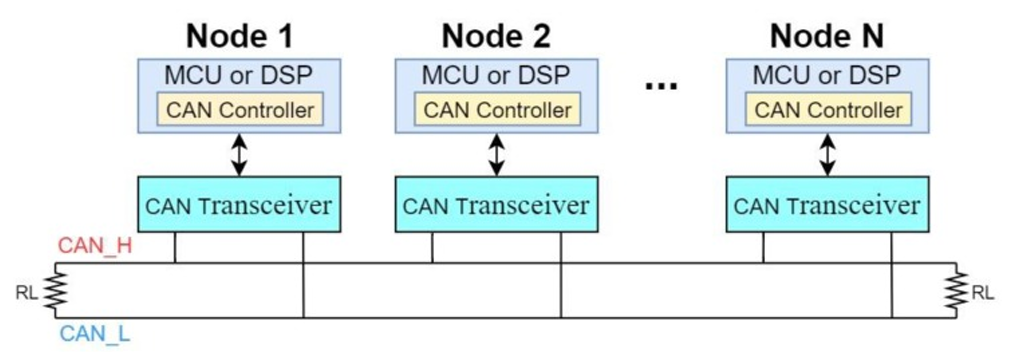
\includegraphics[width=1\textwidth]{images/CAN.png}
	\caption{Mạng CAN tổng quát}
\end{figure}

\subsection{Đặc điểm nổi bật của giao thức CAN}
\begin{itemize}[leftmargin=*]
    \item \textbf{Hoạt động theo mô hình đa master (multi-master):} Mọi thiết bị (node) trên mạng đều có quyền khởi tạo truyền dữ liệu. Điều này giúp mạng CAN linh hoạt hơn so với các mô hình truyền thống chỉ có một master điều khiển.
    \item \textbf{Truyền thông không định địa chỉ thiết bị:} Khác với giao thức UART hoặc I2C, CAN không dùng địa chỉ thiết bị. Thay vào đó, mỗi khung dữ liệu mang một ID (identifier) đại diện cho nội dung thông điệp. Các node sẽ lọc và xử lý dữ liệu theo ID mà chúng quan tâm. Điều này giúp tăng tính linh hoạt và khả năng mở rộng hệ thống.
    \item \textbf{Cơ chế ưu tiên truyền:} Trong trường hợp nhiều node cùng muốn truyền dữ liệu, giao thức CAN sẽ so sánh ID theo bit từng bước để quyết định thiết bị nào được phép tiếp tục truyền. ID có giá trị nhị phân thấp hơn (ưu tiên cao hơn) sẽ giành quyền truy cập bus. Quá trình này gọi là arbitration và diễn ra hoàn toàn tự động mà không gây xung đột.
    \item \textbf{Phát hiện và xử lý lỗi mạnh mẽ:} CAN có nhiều cơ chế phát hiện lỗi như:
    \begin{itemize}
        \item \textit{Bit monitoring:} Kiểm tra sự khác biệt giữa bit gửi và nhận.
        \item \textit{CRC check:} Kiểm tra tính toàn vẹn khung dữ liệu.
        \item \textit{ACK check:} Đảm bảo dữ liệu được ít nhất một node khác nhận thành công.
        \item \textit{Form check:} Kiểm tra định dạng của khung dữ liệu.
    \end{itemize}
    Nếu phát hiện lỗi, node sẽ tự động phát một Error Frame và yêu cầu gửi lại.
    \item \textbf{Tốc độ truyền dữ liệu linh hoạt:} Giao thức CAN hỗ trợ nhiều tốc độ khác nhau tùy theo chiều dài đường truyền. Trên thực tế:
    \begin{itemize}
        \item Với khoảng cách ngắn (dưới 40m), có thể đạt tốc độ tối đa 1 Mbps.
        \item Với khoảng cách dài (lên đến 1 km), tốc độ có thể giảm xuống khoảng 50 kbps.
    \end{itemize}
    Điều này làm cho CAN phù hợp với cả hệ thống nhỏ lẫn hệ thống phân tán rộng.
    \item \textbf{Giao tiếp đồng bộ và thời gian thực:} CAN sử dụng chuẩn mã hóa NRZ (Non-Return to Zero) và kỹ thuật bit stuffing để đồng bộ hóa giữa các node mà không cần xung clock ngoài. Điều này giúp đảm bảo giao tiếp thời gian thực, đặc biệt quan trọng trong các hệ thống an toàn như phanh ABS, điều khiển động cơ hay túi khí.
    \item \textbf{Chi phí thấp, độ tin cậy cao:} Nhờ vào khả năng xử lý lỗi, giảm thiểu dây nối và chi phí phần cứng, CAN trở thành lựa chọn hàng đầu cho các hệ thống nhúng cần độ tin cậy cao với chi phí hợp lý.
\end{itemize}

\section{Nguyên tắc hoạt động}

\subsection{Cấu trúc khung dữ liệu (Data Frame)}
\begin{table}[h!]
\centering
\begin{tabularx}{\textwidth}{l X}
\toprule
\textbf{Trường} & \textbf{Vai trò} \\
\midrule
Start of Frame & Xác định bắt đầu một khung dữ liệu. \\
Arbitration Field & Chứa ID và bit RTR (Remote Transmission Request). \\
Control Field & Xác định độ dài dữ liệu. \\
Data Field & Dữ liệu truyền đi (từ 0 đến 8 byte). \\
CRC Field & Dùng để kiểm tra lỗi dữ liệu truyền. \\
ACK Field & Thiết bị nhận phản hồi xác nhận khung hợp lệ. \\
End of Frame & Đánh dấu kết thúc khung dữ liệu. \\
\bottomrule
\end{tabularx}
\caption{Cấu trúc chi tiết các trường trong Data Frame}
\end{table}

\subsection{Phân loại ID}
Trong giao thức CAN, mỗi khung dữ liệu mang một mã định danh (ID - Identifier) thay vì địa chỉ thiết bị. ID được sử dụng để xác định nội dung thông điệp, phân mức ưu tiên trong quá trình tranh chấp truyền (arbitration) và giúp các node lọc dữ liệu cần thiết.

\begin{itemize}[leftmargin=*]
    \item \textbf{Standard ID (11 bit):}
    Là định dạng gốc của chuẩn CAN theo ISO 11898-1, còn gọi là Base Frame Format. Định dạng này gồm 11 bit, cho phép tối đa $2^{11} = 2048$ mã định danh khác nhau. Thường được sử dụng rộng rãi trong các hệ thống nhỏ, số lượng thiết bị hoặc thông điệp ít. Khung dữ liệu ngắn giúp giảm thời gian truyền, tăng hiệu quả mạng.
    
   quát\begin{figure}[H]
   	\centering
   	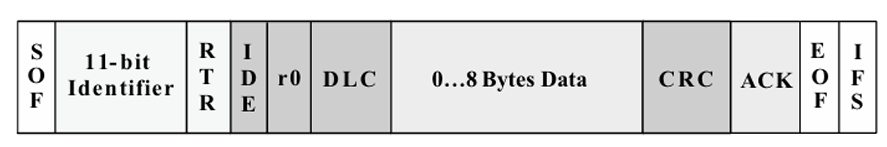
\includegraphics[width=1\textwidth]{images/CAN_ID.png}
   	\caption{Standard CAN: 11-Bit Indentifier}
   \end{figure}

    \item \textbf{Extended ID (29 bit):}
    Mở rộng từ chuẩn CAN cơ bản để đáp ứng nhu cầu phức tạp hơn. Cấu trúc gồm 11 bit gốc + 18 bit mở rộng, tổng cộng 29 bit. Định dạng này cho phép tối đa $2^{29} \approx 537$ triệu mã định danh khác nhau. Thường dùng trong các hệ thống lớn như xe hiện đại, hệ thống công nghiệp quy mô lớn. Hệ thống phân biệt bằng bit điều khiển IDE (Identifier Extension): nếu $\text{IDE} = 1 \Rightarrow$ sử dụng Extended ID.
    
    \begin{figure}[H]
    	\centering
    	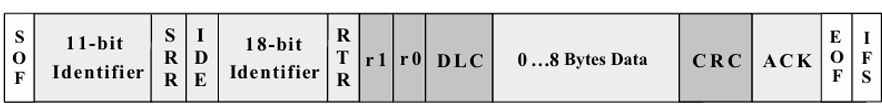
\includegraphics[width=1\textwidth]{images/CAN_EX.png}
    	\caption{Extended CAN: 29-Bit Indentifier}
    \end{figure}
\end{itemize}

\subsection{Truyền và nhận dữ liệu}
\begin{itemize}
    \item Tất cả thiết bị đều giám sát liên tục bus CAN.
    \item Thiết bị bắt đầu truyền khi phát hiện bus rảnh.
    \item Cơ chế arbitration dựa vào ID: thiết bị có ID nhỏ hơn sẽ được ưu tiên.
    \item Sử dụng mã hóa NRZ và kỹ thuật bit stuffing để đảm bảo đồng bộ.
\end{itemize}

\subsection{Phát hiện lỗi}
\begin{itemize}
    \item \textbf{Bit Monitoring:} So sánh bit truyền và bit nhận trên bus.
    \item \textbf{CRC Checking:} Kiểm tra tính toàn vẹn của dữ liệu.
    \item \textbf{Form Checking:} Đảm bảo khung dữ liệu đúng định dạng.
    \item \textbf{ACK Checking:} Thiết bị nhận phải xác nhận bằng cách gửi ACK.
\end{itemize}

\section{Ứng dụng trong Automotive: Hệ thống ô tô}
Trong các phương tiện giao thông hiện đại, đặc biệt là ô tô, giao thức CAN đóng vai trò là xương sống trong mạng truyền thông nội bộ. Với khả năng truyền thông tin hiệu quả, đáng tin cậy và chi phí thấp, CAN đã trở thành tiêu chuẩn công nghiệp trong các hệ thống điện tử trên xe.

\subsection{Các hệ thống tiêu biểu sử dụng giao thức CAN}
\begin{itemize}
    \item \textbf{ECU động cơ (Engine Control Unit):} Điều khiển hoạt động của động cơ như phun nhiên liệu, đánh lửa, kiểm soát khí xả, v.v.
    \item \textbf{Hệ thống túi khí (Airbag System):} Giao tiếp giữa các cảm biến va chạm, bộ xử lý và bộ kích hoạt túi khí để đảm bảo phản ứng tức thời khi xảy ra va chạm.
    \item \textbf{Hệ thống phanh ABS/ESP:} Trao đổi dữ liệu liên tục giữa cảm biến tốc độ bánh xe, ECU phanh và các mô-đun ổn định thân xe để ngăn trượt và lật xe.
    \item \textbf{Hệ thống điều khiển tiện nghi:} Bao gồm điều hòa không khí, điều chỉnh ghế, gương, cửa sổ, đèn nội thất, thường kết nối qua mạng CAN tốc độ thấp (Low-Speed CAN).
    \item \textbf{Màn hình thông tin và giải trí (Infotainment):} Kết nối giữa bảng điều khiển trung tâm, màn hình, bộ định vị GPS, hệ thống âm thanh, và các nút điều khiển trên vô lăng.
\end{itemize}

\subsection{Phân tầng mạng CAN trong ô tô}
Trong thực tế, các hệ thống điện tử trong xe thường được chia thành các tầng mạng CAN khác nhau, tùy vào tốc độ và mức độ quan trọng:
\begin{itemize}
    \item \textbf{High-Speed CAN (500 kbps - 1 Mbps):} Dùng cho các hệ thống an toàn và điều khiển động cơ, yêu cầu tốc độ cao và phản hồi nhanh.
    \item \textbf{Low-Speed / Fault-Tolerant CAN (125 kbps):} Dùng cho các chức năng thân xe như đèn, gương, khóa cửa, nơi yêu cầu tốc độ không quá cao nhưng độ ổn định quan trọng.
    \item \textbf{CAN FD (Flexible Data-rate):} Được tích hợp trong các xe mới để truyền lượng dữ liệu lớn hơn (như từ camera, radar) với tốc độ cao hơn và độ trễ thấp hơn.
\end{itemize}


\chapter{Bảo mật trong hệ thống mạng CAN}

\section{Các vấn đề về bảo mật trong hệ thống mạng CAN}
Mạng CAN (\textit{Controller Area Network}) được thiết kế từ đầu nhằm tối ưu cho tốc độ truyền thông và độ tin cậy trong các hệ thống nhúng, đặc biệt là ô tô. Tuy nhiên, thiết kế ban đầu của CAN không tập trung vào các yêu cầu bảo mật, vì vậy giao thức này tồn tại nhiều lỗ hổng tiềm ẩn khi được đặt trong môi trường kết nối hiện đại.

Dưới đây là một số vấn đề bảo mật chính của mạng CAN:

\begin{itemize}[leftmargin=*]
    \item \textbf{Không có cơ chế xác thực (Authentication):} Bất kỳ thiết bị nào được kết nối vào bus CAN đều có thể gửi thông điệp. Hệ thống không có cách tự nhiên để xác minh nguồn gốc thực sự của thông điệp đó.
    \item \textbf{Không có mã hóa (Encryption):} Dữ liệu trên bus CAN được truyền ở dạng rõ ràng (\textit{plaintext}), tạo điều kiện cho kẻ tấn công nghe lén và phân tích nội dung.
    \item \textbf{Không có phân quyền truy cập (Access Control):} Tất cả các node trên mạng đều chia sẻ cùng một môi trường truyền thông, không có cơ chế kiểm soát vai trò hay đặc quyền truy cập.
    \item \textbf{Dễ bị tấn công từ chối dịch vụ (Denial-of-Service - DoS):} Một thiết bị độc hại có thể liên tục gửi các frame có ID ưu tiên cao để chiếm quyền truy cập bus, làm gián đoạn hoạt động của các node khác.
    \item \textbf{Khả năng nghe trộm (Eavesdropping):} Vì toàn bộ bus chia sẻ chung tín hiệu, mọi node đều có thể quan sát các thông điệp đang lưu thông trên mạng.
    \item \textbf{Dễ bị giả mạo (Spoofing):} Một thiết bị độc hại có thể giả mạo ID của một node hợp lệ để phát thông điệp sai lệch lên mạng.
\end{itemize}

\section{Các phương pháp bảo mật trong hệ thống mạng CAN}
Để khắc phục các hạn chế nêu trên, nhiều giải pháp bảo mật đã được đề xuất. Mỗi phương pháp có ưu điểm và đánh đổi riêng, tùy thuộc vào khả năng phần cứng, yêu cầu thời gian thực và kiến trúc tổng thể của hệ thống.

\subsection{Xác thực thông điệp (Message Authentication)}
\textbf{Nguyên lý.} Một mã xác thực thông điệp (MAC - \textit{Message Authentication Code}) được gắn thêm vào dữ liệu để kiểm tra nguồn gốc và tính toàn vẹn của thông điệp.

\textbf{Cách thực hiện.}
\begin{itemize}[leftmargin=*]
    \item Sử dụng hàm băm kết hợp với khóa bí mật để tạo mã xác thực, ví dụ như HMAC-SHA256.
    \item Node gửi tính giá trị MAC từ dữ liệu và truyền kèm trong payload.
    \item Node nhận tính lại MAC và so sánh với giá trị đã nhận; nếu trùng khớp, thông điệp được xem là hợp lệ.
\end{itemize}

\textbf{Ví dụ.} Với dữ liệu $D$ và khóa $K$, node gửi tính $\text{MAC} = \text{HMAC}_{K}(D)$ rồi gửi cặp $(D, \text{MAC})$. Node nhận tính lại $\text{HMAC}_{K}(D)$ để kiểm tra.

\textbf{Ưu điểm.} Ngăn chặn giả mạo thông điệp. Phát hiện được các sửa đổi trái phép trong quá trình truyền.

\textbf{Nhược điểm.} Không tự chống được tấn công phát lại nếu không kết hợp thêm bộ đếm hoặc dấu thời gian. Làm tăng kích thước payload, dễ chạm giới hạn 8 byte của CAN 2.0. Tăng tải tính toán trên vi điều khiển.

\subsection{Sử dụng bộ đếm tin nhắn đơn giản (Simple Message Counter)}
\textbf{Nguyên lý.} Mỗi thông điệp được gắn một bộ đếm tăng dần để đảm bảo tính ``tươi mới'' (\textit{freshness}). Thiết bị nhận dùng giá trị này để phát hiện và từ chối các bản tin bị phát lại.

\textbf{Cách thực hiện.}
\begin{itemize}[leftmargin=*]
    \item Gắn một trường bộ đếm nhỏ, ví dụ 8 bit hoặc 16 bit, vào thông điệp $M_k$.
    \item Thiết bị nhận lưu giá trị bộ đếm gần nhất cho từng ID hoặc từng phiên giao tiếp.
    \item Nếu bộ đếm trong thông điệp mới không lớn hơn giá trị đã lưu, thông điệp có thể bị xem là bản sao hoặc lỗi thời.
\end{itemize}

\textbf{Ví dụ.} Nếu thông điệp trước đó có bộ đếm là 5 thì thông điệp kế tiếp hợp lệ phải có bộ đếm bằng 6 hoặc lớn hơn.

\textbf{Ưu điểm.} Cơ chế đơn giản, hiệu quả và phù hợp với vi điều khiển giới hạn tài nguyên. Giúp chống lại các cuộc tấn công phát lại ở mức cơ bản.

\textbf{Nhược điểm.} Không tự bảo vệ trước giả mạo hoặc nghe lén nếu không kết hợp với MAC hay mã hóa. Yêu cầu thiết bị nhận phải lưu trạng thái bộ đếm, có thể làm tăng nhu cầu bộ nhớ.

\subsection{Phát hiện xâm nhập (Intrusion Detection System - IDS)}
\textbf{Nguyên lý.} IDS giám sát và phân tích luồng dữ liệu trên bus CAN để phát hiện các hành vi bất thường hoặc độc hại.

\textbf{Cách thực hiện.}
\begin{itemize}[leftmargin=*]
    \item Thu thập dữ liệu CAN và đánh giá bất thường dựa trên tập luật (\textit{rule-based}) hoặc mô hình học máy.
    \item So sánh với hành vi bình thường để phát hiện dấu hiệu lạ như tần suất gửi tăng đột biến hoặc xuất hiện ID không mong đợi.
    \item Gửi cảnh báo hoặc kích hoạt cơ chế chặn khi phát hiện rủi ro.
\end{itemize}

\textbf{Ví dụ.} Nếu một ID thường chỉ gửi 10 thông điệp mỗi phút nhưng đột nhiên phát 100 thông điệp trong vài giây, IDS có thể xem đây là dấu hiệu tấn công.

\textbf{Ưu điểm.} Không đòi hỏi thay đổi sâu vào giao thức CAN gốc. Có khả năng phát hiện các kiểu tấn công mới chưa được định nghĩa trước.

\textbf{Nhược điểm.} Có thể tạo ra cảnh báo giả (\textit{false positive}). Yêu cầu năng lực xử lý tương đối cao nếu dùng mô hình phức tạp.


\chapter{CAN trong ESP32}

\reportsection{4.1 Tổng quan về giao tiếp CAN trên ESP32}

ESP32 là dòng vi điều khiển SoC được sử dụng rộng rãi trong các hệ thống nhúng nhờ tích
hợp đồng thời năng lực xử lý, kết nối không dây và nhiều ngoại vi truyền thông. Bên
cạnh UART, SPI hay I2C, ESP32 còn cung cấp bộ điều khiển CAN cổ điển do Espressif đặt
tên là TWAI (\textit{Two-Wire Automotive Interface}). Đây là nền tảng giúp ESP32 có thể
tham gia trực tiếp vào một mạng CAN thử nghiệm mà không cần bổ sung thêm bộ điều
khiển CAN rời.

\reportsubsection{4.1.1 Bộ điều khiển TWAI}

TWAI trên ESP32 đảm nhiệm lớp điều khiển giao thức của CAN. Khối này xử lý việc đóng
gói khung dữ liệu, phân xử truy cập bus, tạo CRC, xác nhận ACK, theo dõi bộ đếm lỗi và
quản lý các trạng thái truyền thông. Tuy nhiên, TWAI không tạo trực tiếp tín hiệu vi sai
trên đường truyền, vì vậy vẫn cần thêm một CAN transceiver ở lớp vật lý để đưa tín hiệu
ra hai đường CANH và CANL.

\begin{table}[H]
\centering
\begin{tabular}{|p{4.2cm}|p{9.2cm}|}
\hline
\textbf{Thuộc tính} & \textbf{Mô tả} \\ \hline
Chuẩn hỗ trợ & CAN cổ điển theo ISO 11898-1 \\ \hline
Định dạng khung & Standard Frame với ID 11 bit và Extended Frame với ID 29 bit \\ \hline
Dung lượng dữ liệu & Tối đa 8 byte dữ liệu trong mỗi khung \\ \hline
Chức năng tích hợp & Arbitration, CRC, ACK, bộ đếm lỗi, quản lý bus-off và acceptance filter \\ \hline
Khả năng gán chân & Cho phép ánh xạ TX và RX qua GPIO matrix của ESP32 \\ \hline
Giới hạn & Không hỗ trợ CAN FD, do đó không sử dụng payload 64 byte \\ \hline
\end{tabular}
\caption{Đặc điểm chính của giao tiếp TWAI trên ESP32}
\end{table}



\reportsection{4.2 Kiến trúc một nút CAN dùng ESP32}

Một nút CAN sử dụng ESP32 trong đề tài có thể được xem như sự kết hợp giữa khối xử lý
giao thức ở bên trong vi điều khiển và khối phát thu tín hiệu ở bên ngoài. Việc tách rõ hai
khối này đặc biệt quan trọng khi phân tích phần cứng, vì nhiều lỗi triển khai phát sinh từ
nhầm lẫn giữa CAN controller và CAN transceiver.

\reportsubsection{4.2.1 Vai trò của bộ điều khiển CAN}

TWAI đóng vai trò bộ điều khiển CAN nội bộ. Khối này quyết định định dạng khung truyền,
kiểm tra tính hợp lệ của ID, DLC và cờ điều khiển, đồng thời xử lý các cơ chế cốt lõi của
CAN như tranh chấp bus theo mức ưu tiên ID hay tự động phát hiện lỗi. Ở góc nhìn phần
mềm, đây là nơi firmware cấu hình tốc độ bit, chế độ hoạt động và chính sách lọc khung.

\reportsubsection{4.2.2 Vai trò của bộ thu phát CAN}

CAN transceiver là thành phần thuộc lớp vật lý. Nó nhận mức logic TX/RX từ ESP32 rồi
biến đổi thành cặp tín hiệu vi sai CANH/CANL trên bus. Ở chiều ngược lại, transceiver lấy
tín hiệu từ bus và đưa về mức logic để TWAI có thể giải mã. Nếu thiếu transceiver, ESP32
không thể nối trực tiếp vào mạng CAN thực vì không tạo ra được điện áp và đặc tính chống
nhiễu cần thiết của đường truyền vi sai.

\begin{figure}[H]
\centering
\begin{tikzpicture}[
    block/.style={draw, rectangle, minimum width=3.2cm, minimum height=1.1cm, align=center},
    arrow/.style={->, thick}
]
\node[block] (esp) {ESP32\\TWAI Controller};
\node[block, minimum width=4.2cm, right=2.2cm of esp] (trans) {CAN Transceiver\\ TJA1050};
\node[block, minimum width=3.4cm, right=2.2cm of trans] (bus) {CAN Bus\\CANH -- CANL};

\draw[arrow] (esp) -- node[midway, above, align=center, font=\small, fill=white, inner sep=1pt]{Tín hiệu\\TX/RX mức logic} (trans);
\draw[arrow] (trans) -- node[midway, above, align=center, font=\small, fill=white, inner sep=1pt]{Tín hiệu\\vi sai} (bus);
\end{tikzpicture}
\caption{Sơ đồ khối của một nút CAN dùng ESP32}
\end{figure}

\reportsection{4.3 Kết nối phần cứng của mô hình}

Trong mô hình thực nghiệm hiện tại, firmware mặc định sử dụng GPIO26 làm đường truyền
CAN logic và GPIO27 làm đường nhận CAN logic. Hai chân này được nối với module
transceiver ngoài để hình thành một nút CAN hoàn chỉnh.

\begin{table}[H]
\centering
\begin{tabular}{|>{\raggedright\arraybackslash}p{3.2cm}|>{\raggedright\arraybackslash}p{2.4cm}|>{\raggedright\arraybackslash}p{3.2cm}|>{\raggedright\arraybackslash}p{4.2cm}|}
\hline
\textbf{Nhóm tín hiệu} & \textbf{ESP32} & \textbf{Transceiver} & \textbf{Vai trò} \\ \hline
Truyền dữ liệu & GPIO26 & TXD & Đưa dữ liệu từ TWAI sang bộ thu phát \\ \hline
Nhận dữ liệu & GPIO27 & RXD & Đưa dữ liệu từ bộ thu phát về TWAI \\ \hline
Nguồn nuôi & 3.3 V hoặc 5 V & VCC & Phụ thuộc loại module transceiver sử dụng \\ \hline
Mass chung & GND & GND & Tạo mốc điện áp chung cho toàn nút \\ \hline
Đường bus & -- & CANH, CANL & Kết nối ra đường truyền vi sai của mạng CAN \\ \hline
\end{tabular}
\caption{Ánh xạ chân CAN trong mô hình ESP32 của đề tài}
\end{table}

\reportsection{4.4 Cấu trúc và nguyên lý hoạt động của TWAI}

Khối TWAI trong ESP32 có thể được nhìn nhận như tập hợp của nhiều khối chức năng phối
hợp với nhau để hoàn thành quá trình truyền thông CAN. Cách phân rã này giúp việc mô tả
vai trò của phần cứng rõ ràng hơn và phù hợp với cách trình bày học thuật trong báo cáo.

\reportsubsection{4.4.1 Các khối chức năng chính}

\begin{itemize}[leftmargin=1.5cm, itemsep=0.6em]
    \item Khối điều khiển chế độ hoạt động quyết định TWAI đang ở trạng thái truyền nhận
    bình thường, chỉ nghe hoặc kiểm thử không cần ACK.
    \item Khối định thời bit thiết lập tốc độ truyền và các tham số đồng bộ để mọi nút trên
    bus có cùng nhịp giao tiếp.
    \item Khối truyền chịu trách nhiệm phát khung lên bus, phối hợp với cơ chế arbitration
    và theo dõi việc bản tin có được xác nhận thành công hay không.
    \item Khối nhận lấy tín hiệu từ transceiver, giải mã thành khung CAN rồi chuyển dữ liệu
    cho tầng driver phần mềm.
    \item Khối acceptance filter loại bỏ hoặc cho phép các khung theo cấu hình tiếp nhận.
    \item Khối quản lý lỗi duy trì các bộ đếm lỗi, phát hiện bus-off và hỗ trợ chẩn đoán khi
    đường truyền gặp sự cố.
\end{itemize}

\reportsubsection{4.4.2 Quy trình khởi tạo và trao đổi dữ liệu}

Ở mức tổng quát, một nút ESP32 tham gia mạng CAN thường đi qua các bước sau:

\begin{enumerate}
    \item Chọn cặp chân GPIO dùng cho đường TX và RX của TWAI.
    \item Thiết lập tốc độ bit và cấu hình chế độ hoạt động phù hợp với vai trò của nút.
    \item Đặt chính sách lọc khung để xác định phạm vi bản tin cần tiếp nhận.
    \item Khởi động driver TWAI và đưa transceiver vào trạng thái sẵn sàng làm việc.
    \item Thực hiện truyền hoặc nhận khung thông qua hàng đợi của driver.
    \item Theo dõi trạng thái lỗi để kịp thời xử lý khi bus xuất hiện bất thường.
\end{enumerate}

\begin{figure}[H]
\centering
\begin{tikzpicture}[
    node distance=1.15cm,
    block/.style={draw, rectangle, rounded corners, minimum width=8.0cm, minimum height=0.85cm, align=center},
    setupblock/.style={block, fill=blue!12},
    startblock/.style={block, fill=green!12},
    runblock/.style={block, fill=yellow!15},
    arrow/.style={->, thick}
]
\node[setupblock] (s1) {Chọn chân TX/RX và kết nối với transceiver};
\node[setupblock, below of=s1] (s2) {Thiết lập tốc độ bit, chế độ hoạt động và bộ lọc khung};
\node[startblock, below of=s2] (s3) {Khởi động TWAI và đưa nút vào trạng thái sẵn sàng};
\node[runblock, below of=s3] (s4) {Truyền hoặc nhận bản tin CAN trên bus};
\node[runblock, below of=s4] (s5) {Kiểm tra trạng thái lỗi và cập nhật xử lý tầng trên};

\draw[arrow] (s1) -- (s2);
\draw[arrow] (s2) -- (s3);
\draw[arrow] (s3) -- (s4);
\draw[arrow] (s4) -- (s5);
\end{tikzpicture}
\caption{Quy trình tổng quát khi khởi tạo và vận hành TWAI trên ESP32}
\end{figure}

\reportsection{4.5 Các tham số cấu hình quan trọng}

Để một nút ESP32 giao tiếp ổn định trên bus CAN, một số tham số cấu hình có ý nghĩa quyết
định gồm chế độ hoạt động, tốc độ bit và chính sách lọc khung. Đây cũng là ba nhóm tham
số ảnh hưởng trực tiếp đến việc nút được dùng như ECU mô phỏng, nút tấn công hay nút
giám sát trong hệ thống CyberCAN Defense.

\reportsubsection{4.5.1 Chế độ hoạt động}

\begin{itemize}
    \item \textbf{Normal mode:} nút có thể truyền, nhận và phản hồi ACK như một thành
    phần hoạt động bình thường trên bus.
    \item \textbf{No ACK mode:} hữu ích khi kiểm thử đơn lẻ trong môi trường chưa có nút
    khác xác nhận bản tin, nhưng không phù hợp cho vận hành thực tế.
    \item \textbf{Listen Only mode:} nút chỉ nghe bus, không phát bản tin và không gửi ACK,
    phù hợp với vai trò giám sát hoặc IDS vì không làm thay đổi lưu lượng trên bus.
\end{itemize}

Trong phạm vi đề tài, Normal mode phù hợp với các nút đóng vai trò ECU mô phỏng hoặc
nút phát tấn công, còn Listen Only mode phù hợp với các nút chuyên quan sát và thu thập
log để phân tích.

\reportsubsection{4.5.2 Tốc độ bit và sự đồng bộ trên bus}

Tất cả các nút trên cùng bus CAN phải sử dụng cùng tốc độ bit; nếu không, bản tin sẽ
không được giải mã đúng và mạng nhanh chóng phát sinh lỗi. Một số tốc độ thường gặp
được trình bày trong Bảng 4.3.

\begin{table}[H]
\centering
\begin{tabular}{|p{3cm}|p{9.6cm}|}
\hline
\textbf{Tốc độ bit} & \textbf{Ý nghĩa sử dụng} \\ \hline
125 kbps & Phù hợp với mạng tốc độ thấp hoặc đường truyền dài hơn \\ \hline
250 kbps & Thường dùng trong các mô hình nhúng và công nghiệp quy mô nhỏ \\ \hline
\rowcolor{red!20}
500 kbps & Cân bằng giữa tốc độ và độ ổn định, phù hợp với mô hình thí nghiệm của đề tài \\ \hline
1 Mbps & Dùng cho môi trường cự ly ngắn, yêu cầu băng thông cao hơn \\ \hline
\end{tabular}
\caption{Một số tốc độ bit CAN thường gặp}
\end{table}

Mô hình CyberCAN Defense lựa chọn 500 kbps vì đây là mức cấu hình phổ biến, đủ nhanh
để tái hiện các tình huống tấn công như replay hay flood, đồng thời vẫn ổn định với hệ
thống dây nối ngắn trên bàn thí nghiệm.

\reportsection{4.6 Truyền nhận trên ESP32}

Ở phía truyền, firmware chuẩn bị bản tin bằng cách xác định ID, độ dài dữ liệu, kiểu khung
và nội dung payload trước khi đưa vào hàng đợi của driver. Bộ điều khiển TWAI sau đó
thực hiện phát bản tin lên bus và tự động tham gia cơ chế arbitration nếu cùng lúc có nhiều
nút muốn truyền. Ở phía nhận, các khung hợp lệ được giải mã và chuyển vào hàng đợi nhận
để phần mềm tầng trên đọc ra xử lý. Cách tổ chức này đặc biệt phù hợp với hệ thống có
nhiều tác vụ đồng thời như đề tài hiện tại, nơi việc truyền bản tin, phát hiện tấn công và gửi
log có thể diễn ra song song.

Trong CAN cổ điển, một khung dữ liệu có thể dùng Standard ID 11 bit hoặc Extended ID
29 bit. Việc lựa chọn kiểu ID cần được thống nhất ngay từ giai đoạn thiết kế hệ thống để
tránh sai khác khi các nút giao tiếp chéo với nhau.



\chapter{Thiết kế hệ thống}

% ============================================================
\reportsection{5.1 Hệ thống phần cứng}
% ============================================================

Kiến trúc phần cứng của đề tài được xây dựng theo mô hình tối giản nhưng đầy đủ
để thể hiện một mạng CAN thử nghiệm có khả năng sinh tấn công và phát hiện bất
thường. Mỗi nút CAN gồm một vi điều khiển ESP32 kết hợp với module thu phát CAN
TJA1050. Máy tính đóng vai trò điều khiển và giám sát, kết nối với ESP32 qua cổng
USB--UART; ứng dụng web trên máy tính không tham gia trực tiếp vào bus vật lý mà
gửi lệnh và nhận log phản hồi theo thời gian thực.

% ----------------------------------------------------------
\reportsubsection{5.1.1 ESP32}
% ----------------------------------------------------------

ESP32 đảm nhận toàn bộ phần xử lý điều khiển của nút. Firmware được nạp qua
PlatformIO với framework Arduino. Trong quá trình khởi động, ESP32 mở cổng UART
ở tốc độ 115.200 bps để phục vụ terminal và ghi log, đồng thời khởi tạo bộ điều
khiển CAN ở tốc độ 500 kbps.


\begin{table}[H]
\centering
\begin{tabular}{|>{\raggedright\arraybackslash}p{5cm}|>{\raggedright\arraybackslash}p{3cm}|>{\raggedright\arraybackslash}p{5.5cm}|}
\hline
\textbf{Tham số} & \textbf{Giá trị} & \textbf{Ghi chú} \\ \hline
Tốc độ CAN & 500 kbps & Phù hợp cho mô hình thử nghiệm \\ \hline
Chân TX CAN & GPIO 26 & Kết nối tới TXD của transceiver \\ \hline
Chân RX CAN & GPIO 27 & Kết nối tới RXD của transceiver \\ \hline
Tốc độ UART & 115.200 bps & Terminal và ghi log \\ \hline
Bảo vệ bộ đếm & Bật & Byte cuối mỗi khung là số thứ tự \\ \hline
Kích thước payload tối đa & 7 byte & Byte thứ 8 dành cho bộ đếm \\ \hline
Số ID theo dõi đồng thời & 16 & Giới hạn bộ nhớ của cấu trúc tracker \\ \hline
\end{tabular}
\caption{Cấu hình mặc định của firmware ESP32}
\end{table}

Vòng lặp chính của chương trình thực hiện tuần hoàn năm công việc: đọc lệnh từ
UART, thăm dò khung CAN mới từ bus, cập nhật các tác vụ tấn công định kỳ, điều
khiển LED báo hoạt động và phục vụ dấu nhắc terminal. Nhờ cách tổ chức vòng lặp
đơn luồng này, ESP32 vừa đóng vai trò nút truyền thông CAN vừa là bộ xử lý cục
bộ cho các thuật toán phát hiện xâm nhập.

% ----------------------------------------------------------
\reportsubsection{5.1.2 Module CAN TJA1050}
% ----------------------------------------------------------

TJA1050 là IC thu phát CAN của NXP Semiconductors, đảm nhận lớp vật lý theo chuẩn
ISO 11898-2. Trong mô hình của đề tài, TJA1050 thường được tích hợp sẵn trên một
board nhỏ có kèm điện trở kéo và tụ lọc. Phần tử này nhận tín hiệu logic từ GPIO
của ESP32, biến đổi thành cặp tín hiệu vi sai CANH/CANL và ngược lại. Các thông
số kỹ thuật chính được trình bày trong Bảng~5.2.

\begin{figure}[H]
        \centering
        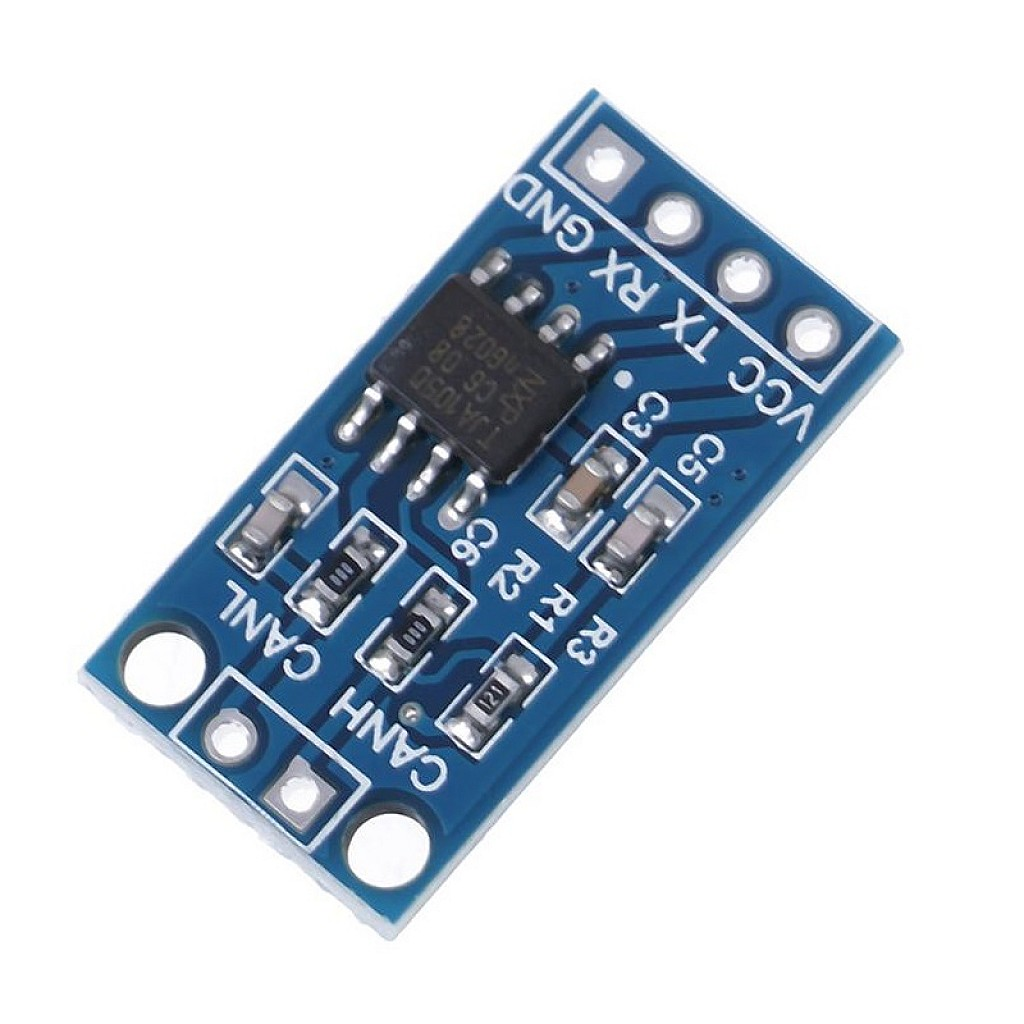
\includegraphics[width=0.5\textwidth]{images/TJA.png}
        \caption{Module CAN TJA1050}
    \end{figure}

\begin{table}[H]
\centering
\begin{tabular}{|>{\raggedright\arraybackslash}p{4.5cm}|>{\raggedright\arraybackslash}p{8.5cm}|}
\hline
\textbf{Thuộc tính} & \textbf{Mô tả} \\ \hline
Chuẩn giao tiếp & ISO 11898, CAN 2.0A/B \\ \hline
Điện áp cấp nguồn & 4,75 V -- 5,25 V (danh nghĩa 5 V) \\ \hline
Mức logic đầu vào & Tương thích 3,3 V và 5 V \\ \hline
Tốc độ tối đa & 1 Mbps \\ \hline
Chân kết nối chính & TXD, RXD, VCC, GND, CANH, CANL \\ \hline
Điện trở kết thúc bus & $120~\Omega$ tại mỗi đầu bus \\ \hline
\end{tabular}
\caption{Đặc điểm kỹ thuật của module TJA1050}
\end{table}

Một lưu ý quan trọng khi ghép ESP32 (3,3 V) với TJA1050 (5 V) là mức điện áp ngõ
ra của transceiver trả về GPIO của ESP32 có thể ở mức 5 V tùy phiên bản module.
Trong trường hợp này, cần sử dụng phân áp điện trở hoặc IC dịch mức logic để
bảo vệ vi điều khiển.

% ----------------------------------------------------------
\reportsubsection{5.1.3 Sơ đồ kết nối phần cứng}
% ----------------------------------------------------------

Sơ đồ kết nối giữa ESP32 và module TJA1050 được thể hiện trong Hình~5.1. Chân GPIO
26 của ESP32 làm đường truyền CAN logic, chân GPIO 27 làm đường nhận; hai chân này
nối trực tiếp tới các ngõ vào/ra tương ứng của transceiver. Từ transceiver, cặp
đường CANH/CANL đi ra bus chung

    \begin{figure}[H]
        \centering
        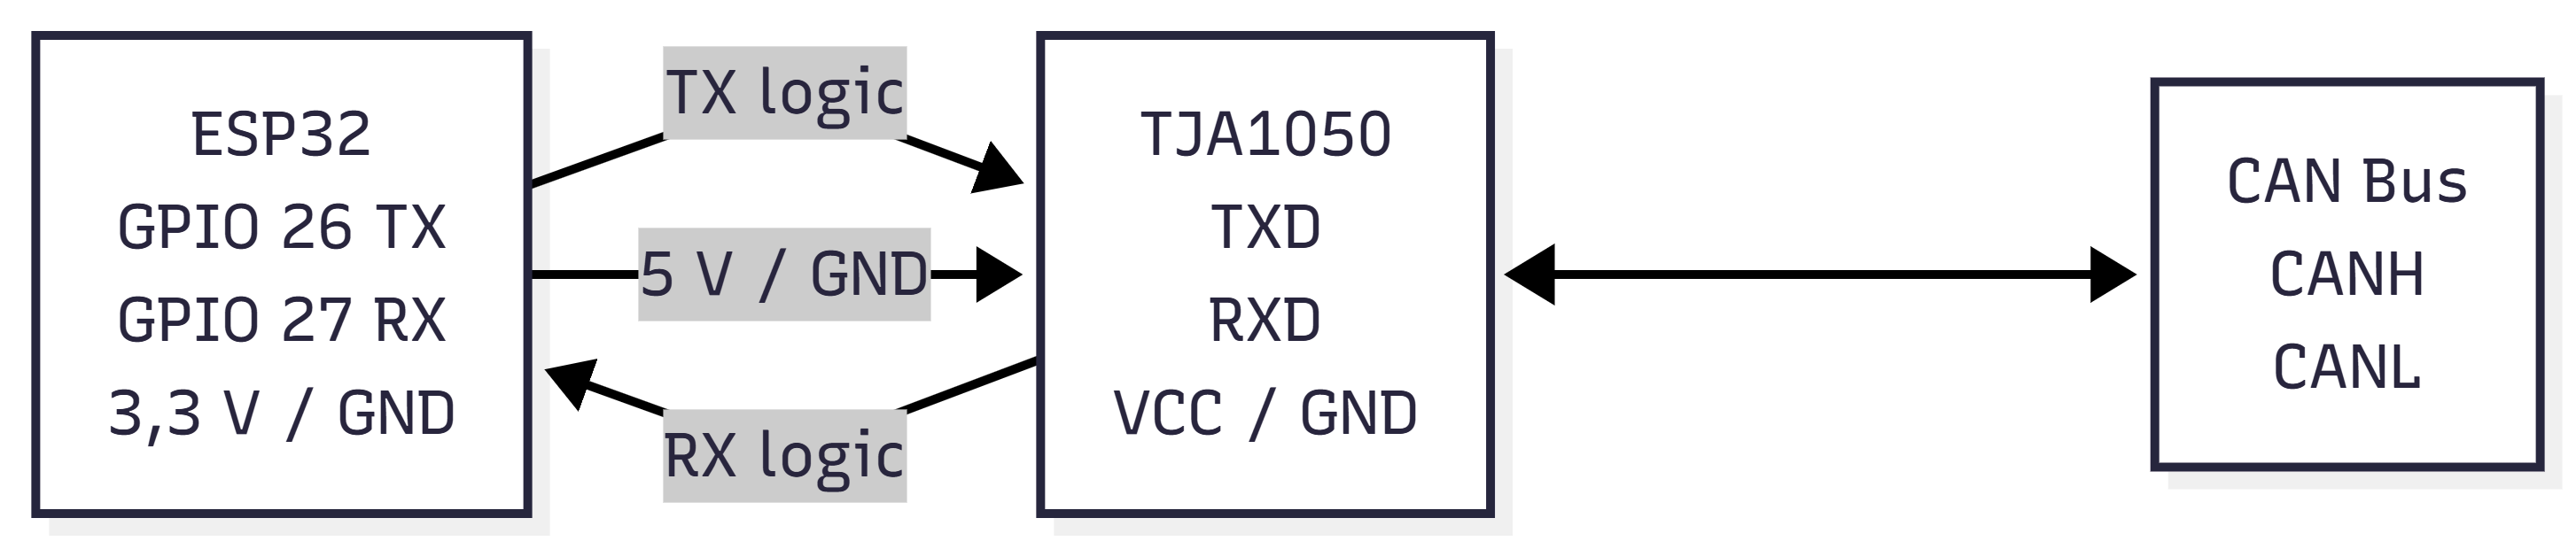
\includegraphics[width=0.85\textwidth]{images/so-do-ket-noi.png}
        \caption{Sơ đồ khối phần cứng tổng quan}
\end{figure}
% ============================================================
\reportsection{5.2 Hệ thống phần mềm}
% ============================================================

Hệ thống phần mềm được chia thành hai lớp phối hợp qua giao tiếp UART và
HTTP/WebSocket. Lớp thứ nhất là firmware nhúng chạy trực tiếp trên ESP32, chịu
trách nhiệm giao tiếp CAN, mô phỏng tấn công và phát hiện bất thường. Lớp thứ hai
là ứng dụng web chạy trên máy tính, đóng vai trò giao diện điều khiển và giám sát
thời gian thực. Kiến trúc tổng thể được mô tả trong Hình~5.3.

% ```mermaid
% graph TD
%     subgraph Firmware [Lớp Firmware ESP32]
%         direction LR
%         m1[Khởi động vòng lặp]
%         m2[Giao tiếp CAN]
%         m3[Terminal UART]
%         m4[Mô phỏng tấn công]
%         m5[Phát hiện xâm nhập]
%         m6[Ghi log]
%         m7[Quản lý trạng thái]
%         
%         m1 --> m2 & m3 & m4
%         m2 --> m5 & m6
%         m5 --> m7
%     end
%     
%     subgraph Web [Lớp Ứng dụng Web]
%         direction LR
%         w1[REST API]
%         w2[WebSocket]
%         w3[Mô phỏng phần mềm]
%         w4[Giao diện người dùng]
%         
%         w1 --> w2 --> w3
%     end
%     
%     m3 -. "UART 115.200 bps" .-> Web
%     Web -. "HTTP / WebSocket" .-> Firmware
% ```
\IfFileExists{images/kien-truc-phan-mem.png}{%
    \begin{figure}[H]
        \centering
        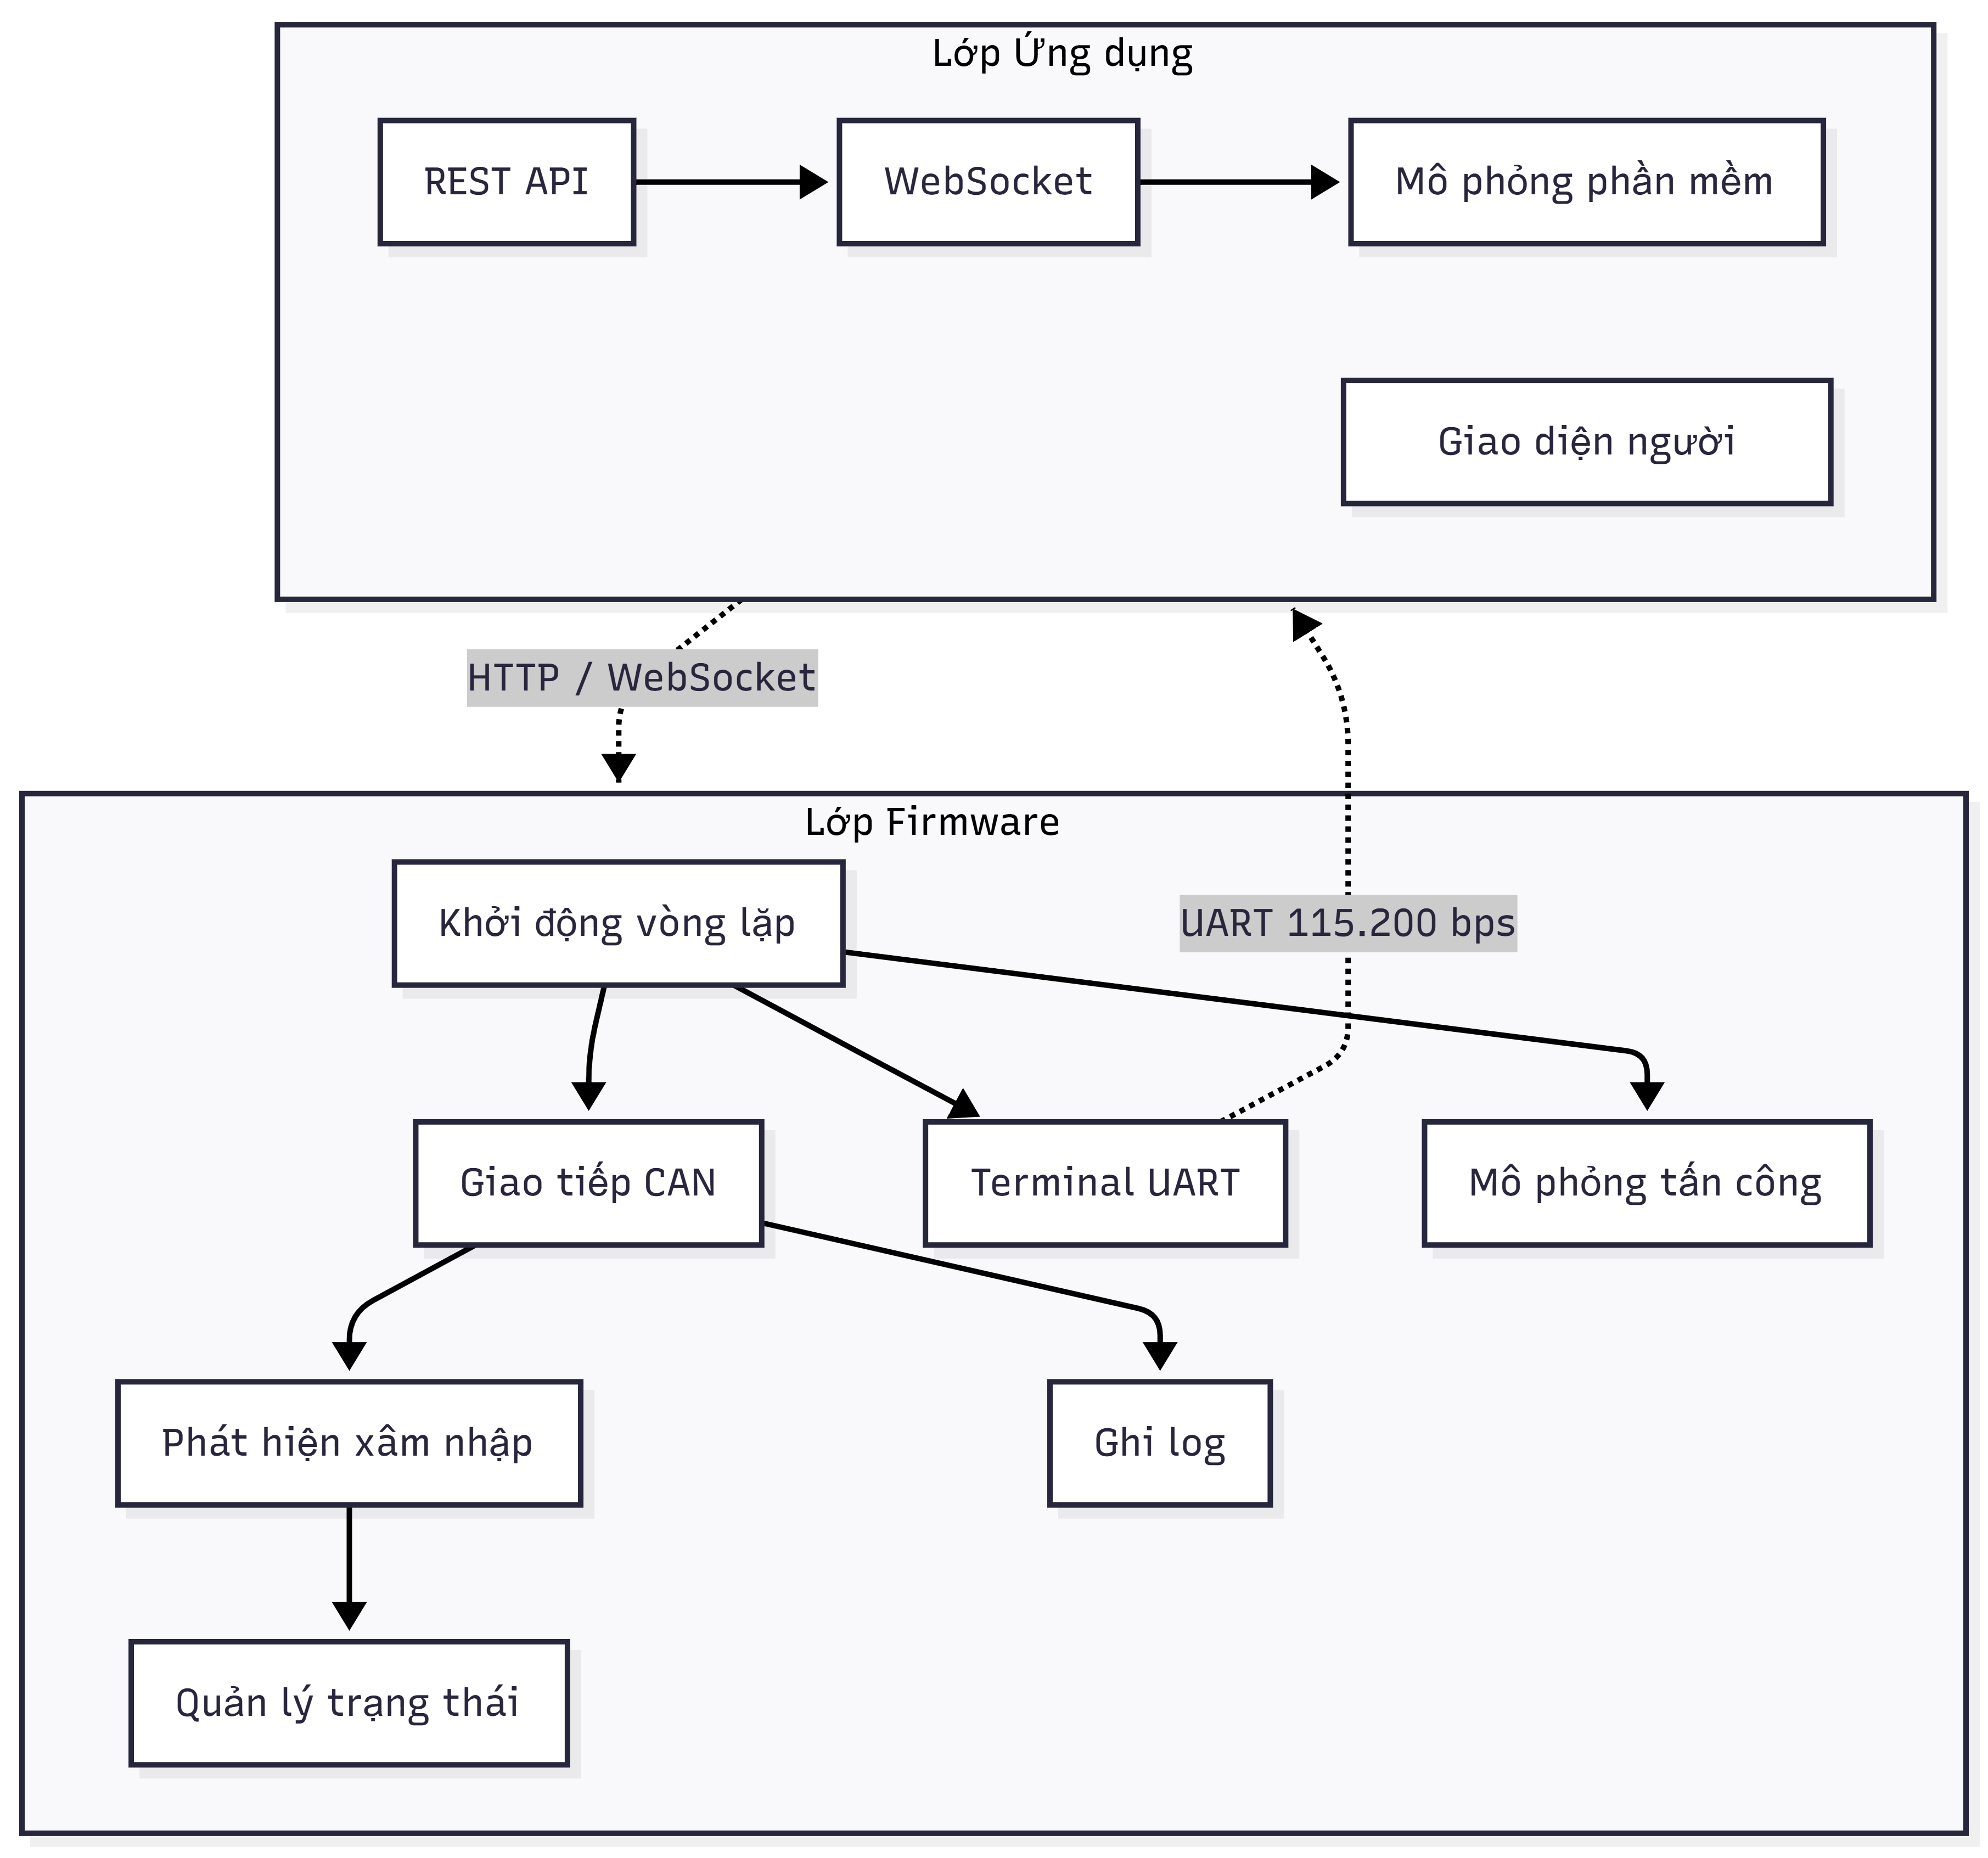
\includegraphics[width=0.85\textwidth]{images/kien-truc-phan-mem.png}
        \caption{Kiến trúc tổng thể hai lớp phần mềm của hệ thống}
    \end{figure}
}{%
    \IfFileExists{images/kien-truc-phan-mem.jpg}{%
        \begin{figure}[H]
            \centering
            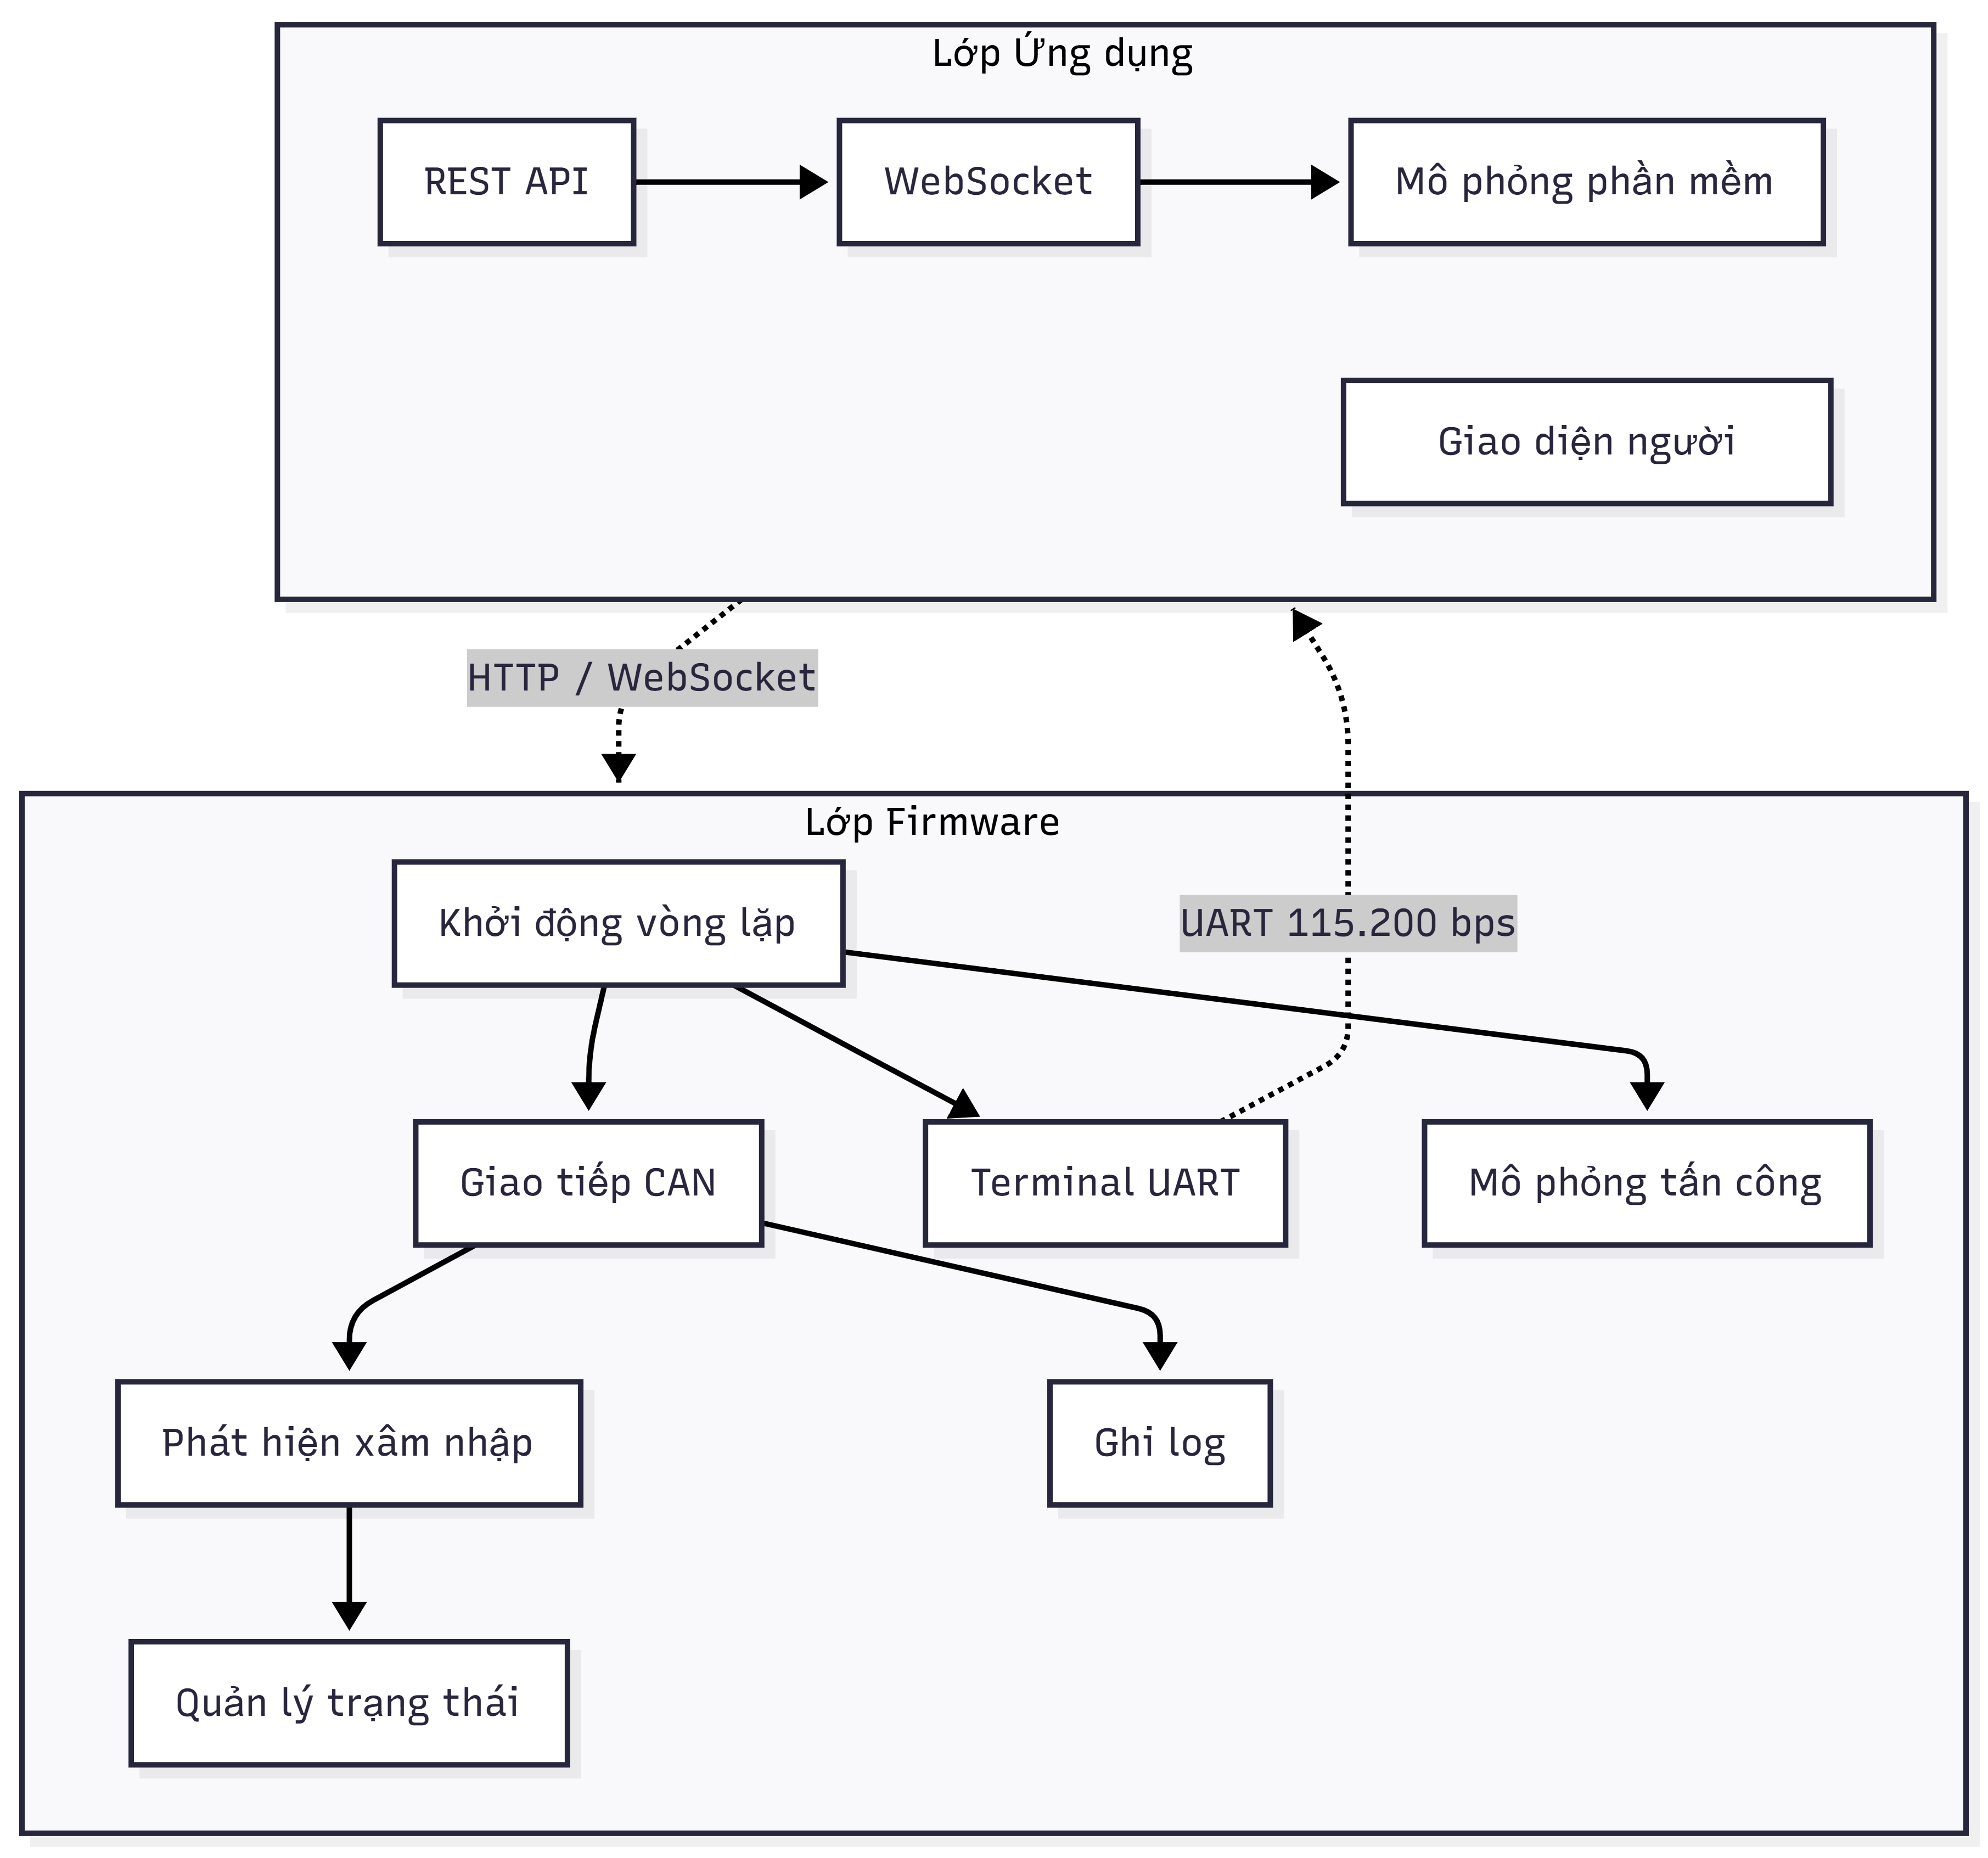
\includegraphics[width=0.85\textwidth]{images/kien-truc-phan-mem.jpg}
            \caption{Kiến trúc tổng thể hai lớp phần mềm của hệ thống}
        \end{figure}
    }{%
        \placeholderfigure{%
            Ảnh kiến trúc tổng thể hai lớp phần mềm của hệ thống.\\
            Đặt ảnh tại \texttt{report/images/kien-truc-phan-mem.png} hoặc \texttt{.jpg}%
        }{Kiến trúc tổng thể hai lớp phần mềm của hệ thống}
    }%
}

% ----------------------------------------------------------
\reportsubsection{5.2.1 Firmware ESP32}
% ----------------------------------------------------------

Firmware được tổ chức thành bảy mô-đun, mỗi mô-đun phụ trách một nhóm chức năng
độc lập. Các mô-đun giao tiếp với nhau qua một tập hợp biến trạng thái chia sẻ,
cho phép toàn bộ hệ thống hoạt động trong một luồng đơn mà không cần cơ chế đồng
bộ phức tạp.

\begin{table}[H]
\centering
\begin{tabular}{|>{\raggedright\arraybackslash}p{5cm}|>{\raggedright\arraybackslash}p{8.5cm}|}
\hline
\textbf{Mô-đun} & \textbf{Vai trò} \\ \hline
Khởi động và vòng lặp chính & Điều phối toàn bộ luồng xử lý của firmware \\ \hline
Giao tiếp CAN & Khởi tạo bus, gửi và nhận khung, bảo vệ bộ đếm \\ \hline
Xử lý lệnh terminal & Phân tích lệnh UART, in trạng thái hệ thống \\ \hline
Mô phỏng tấn công & Quản lý và thực thi năm loại tác vụ tấn công định kỳ \\ \hline
Phát hiện xâm nhập & Phân tích hành vi khung, sinh cảnh báo, quản lý luật chặn \\ \hline
Ghi log & Định dạng và xuất thông điệp ra UART theo chuẩn thống nhất \\ \hline
Quản lý trạng thái & Lưu trữ toàn bộ dữ liệu vận hành trong RAM nội bộ \\ \hline
\end{tabular}
\caption{Các mô-đun firmware và vai trò}
\end{table}

Các kiểu dữ liệu trung tâm được khai báo tập trung trong một tệp tiêu đề chung, bao
gồm cấu trúc khung CAN, bản ghi cảnh báo, khung được bắt gần nhất, các tác vụ tấn
công, bộ theo dõi từng ID và các cấu trúc phòng thủ. Nhờ đó, toàn bộ mô-đun chia
sẻ cùng một biểu diễn dữ liệu và giảm sự phụ thuộc lẫn nhau.

% ----------------------------------------------------------
\reportsubsection{5.2.2 Giao diện CAN và cơ chế bảo vệ bộ đếm}
% ----------------------------------------------------------

Mọi khung do người dùng tạo ra đều được kiểm tra và chuẩn hóa trước khi phát lên
bus. Quá trình này bao gồm: xác nhận CAN ID nằm trong phạm vi hợp lệ, kiểm tra độ
dài dữ liệu, và tự động chèn thêm một byte số thứ tự tăng dần vào cuối payload.
Nhờ đó, mỗi khung hợp lệ trên bus luôn mang một bộ đếm phân biệt giúp phát hiện
hành vi phát lại.

Ở phía nhận, mô-đun giao tiếp CAN đọc khung từ bus theo từng lô nhỏ. Mỗi khung
nhận được lần lượt qua các bước xử lý: kiểm tra xem ID có đang bị chặn bởi
cơ chế phòng thủ hay không, ghi log, phân tích bởi hệ thống phát hiện xâm nhập và
lưu lại làm khung bắt gần nhất để phục vụ tính năng replay.

% ----------------------------------------------------------
\reportsubsection{5.2.3 Hệ thống phát hiện xâm nhập (IDS)}
% ----------------------------------------------------------

Hệ thống phát hiện xâm nhập hoạt động theo hai cấp độ theo dõi song song. Ở cấp
độ đầu tiên, mỗi CAN ID trên bus được theo dõi riêng biệt bởi một bộ theo dõi
(tracker) lưu trữ lịch sử về tần suất xuất hiện, nội dung payload, bộ đếm thứ tự
và đường cơ sở bình thường. Hệ thống duy trì đồng thời tối đa 16 bộ theo dõi; khi
số ID vượt quá giới hạn, bộ theo dõi của ID ít hoạt động nhất sẽ được tái sử dụng.

Ở cấp độ thứ hai, một bộ theo dõi lưu lượng toàn cục quan sát hành vi tổng thể của
toàn bộ bus trong một cửa sổ thời gian trượt, ghi nhận số lượng ID mới và mức độ
thay đổi ID liên tiếp -- hai chỉ số đặc trưng của tấn công Fuzzing.

\begin{table}[H]
\centering
\begin{tabular}{|>{\raggedright\arraybackslash}p{3.6cm}|>{\raggedright\arraybackslash}p{3.8cm}|>{\raggedright\arraybackslash}p{6cm}|}
\hline
\textbf{Loại cảnh báo} & \textbf{Phương pháp phát hiện} & \textbf{Điều kiện kích hoạt} \\ \hline
Replay (phát lại) & So sánh bộ đếm & Byte số thứ tự không tăng đúng thứ tự \\ \hline
DoS (ngập lưu lượng) & Ước tính tốc độ & Tốc độ cùng ID $>$ 60 khung/giây \\ \hline
Fuzzing (quét ngẫu nhiên) & Theo dõi toàn bus & $\geq$ 4 ID mới, $\geq$ 5 đổi ID / 1,2 giây \\ \hline
Spoofing (giả mạo) & So sánh baseline & Payload lệch $\geq$ 2 byte so với mẫu bình thường \\ \hline
\end{tabular}
\caption{Tổng hợp các loại cảnh báo IDS và điều kiện kích hoạt}
\end{table}

% ----------------------------------------------------------
\reportsubsection{5.2.4 Bộ mô phỏng tấn công}
% ----------------------------------------------------------

Bộ mô phỏng tấn công cung cấp năm kiểu tấn công có thể kích hoạt độc lập qua
terminal UART hoặc giao diện web. Mỗi kiểu tấn công chạy như một tác vụ định kỳ
trong vòng lặp chính với chu kỳ có thể tùy chỉnh.

\begin{table}[H]
\centering
\begin{tabular}{|>{\raggedright\arraybackslash}p{2.5cm}|>{\raggedright\arraybackslash}p{2.5cm}|>{\raggedright\arraybackslash}p{8cm}|}
\hline
\textbf{Kiểu tấn công} & \textbf{Chu kỳ mặc định} & \textbf{Mô tả} \\ \hline
Replay & 250 ms & Phát lại nguyên bản khung hợp lệ đã bắt được, kể cả bộ đếm cũ \\ \hline
DoS & 20 ms & Ngập lưu lượng trên một CAN ID với tần suất cao \\ \hline
Fuzzing & 35 ms & Phát liên tục các khung với ID và payload ngẫu nhiên \\ \hline
Spoofing & 120 ms & Giả mạo ID của bản tin hợp lệ với nội dung bị biến đổi \\ \hline
\end{tabular}
\caption{Các kiểu tấn công được hỗ trợ}
\end{table}

Tấn công Replay có đặc điểm nổi bật là phát lại khung ở mức thô (wire level), tức
là không qua bước chuẩn hóa và bổ sung bộ đếm mới. Điều này khiến byte số thứ tự
bị lặp lại, tạo điều kiện cho IDS phát hiện. Tấn công Fuzzing sử dụng bộ sinh số
giả ngẫu nhiên để tạo ra các CAN ID và payload biến đổi liên tục trong mỗi chu kỳ.
Tấn công Spoofing dùng ID của một bản tin hợp lệ đã biết nhưng biến đổi nội dung
theo một mẫu xoay vòng qua từng chu kỳ phát.

% ----------------------------------------------------------
\reportsubsection{5.2.5 Ứng dụng web giám sát và điều khiển}
% ----------------------------------------------------------

Ứng dụng web sử dụng FastAPI làm backend và HTML/CSS/JavaScript thuần túy làm
giao diện người dùng. Hệ thống được khởi động dưới dạng máy chủ web tại cổng 8000,
phục vụ đồng thời giao diện HTML và luồng dữ liệu thời gian thực qua WebSocket.

Backend phân biệt hai chế độ kết nối nút. Trong chế độ phần cứng thực, backend
chuyển tiếp lệnh văn bản tới firmware qua cổng nối tiếp. Trong chế độ mô phỏng
phần mềm, backend tự sinh luồng sự kiện tấn công và phản hồi IDS mà không cần
phần cứng thực, phục vụ cho việc trình diễn giao diện. Giao diện web cung cấp đầy
đủ chức năng thêm/xóa nút, gửi khung CAN, kích hoạt từng kiểu tấn công và bật/tắt
cơ chế phòng thủ. Toàn bộ log và sự kiện được phát trực tiếp tới trình duyệt theo
thời gian thực qua kênh WebSocket.

% Gợi ý ảnh: chụp màn hình giao diện web đang hiển thị log và các nút điều khiển
% Đặt tại: report/images/web-interface.png hoặc .jpg
\IfFileExists{images/web-interface.png}{%
    \begin{figure}[H]
        \centering
        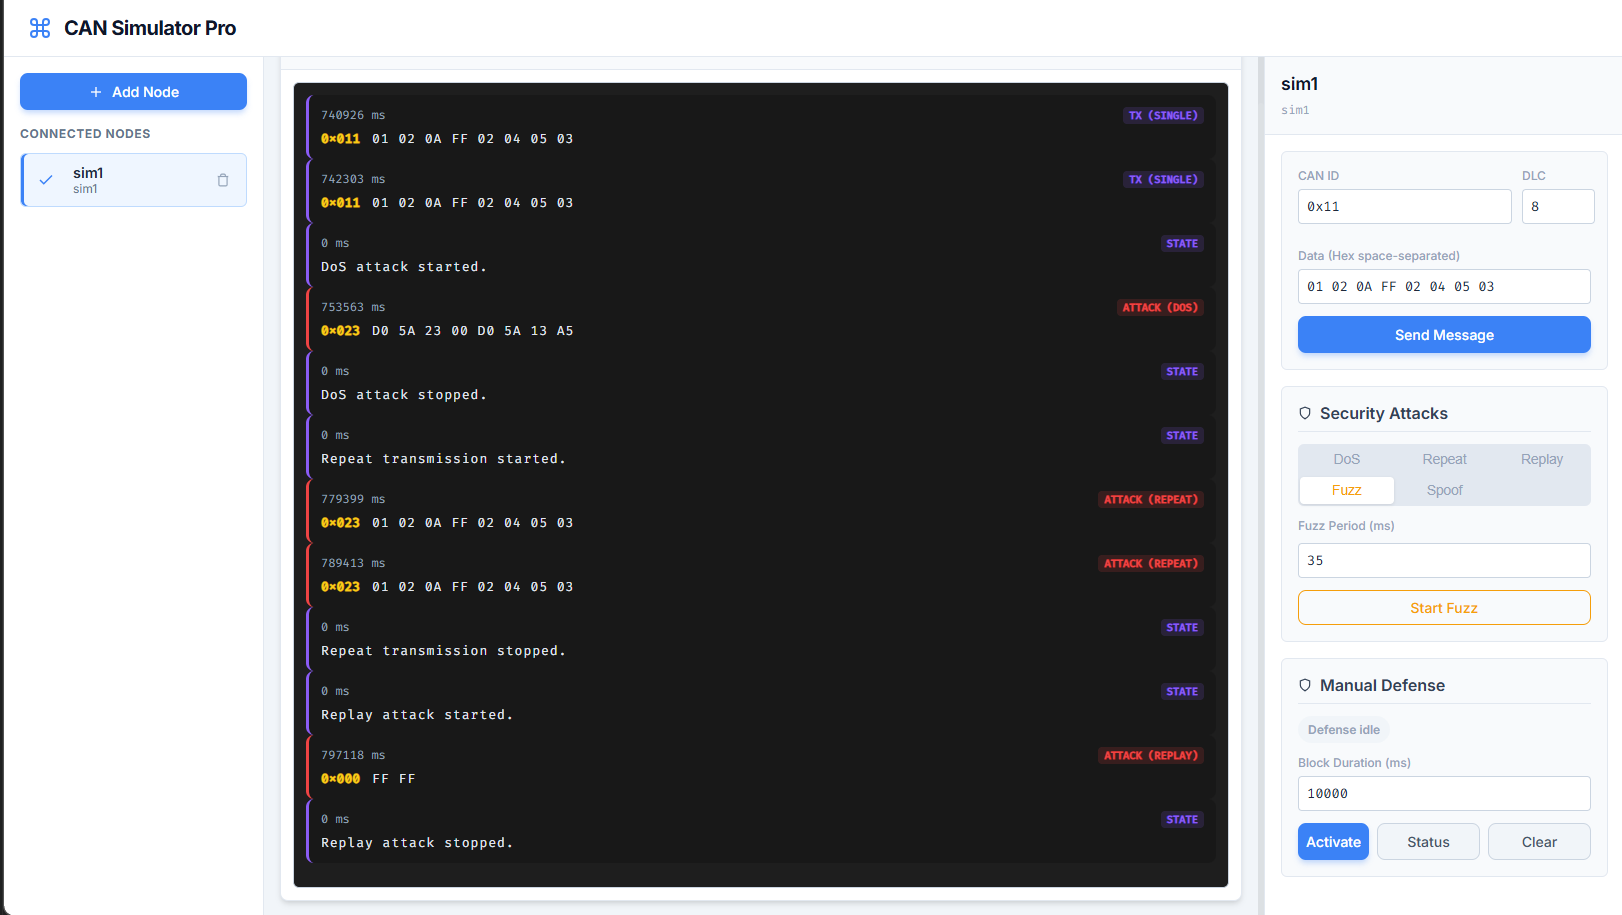
\includegraphics[width=0.88\textwidth]{images/web-interface.png}
        \caption{Giao diện web giám sát, tấn công và phòng thủ CAN}
    \end{figure}
}{%
    \IfFileExists{images/web-interface.jpg}{%
        \begin{figure}[H]
            \centering
            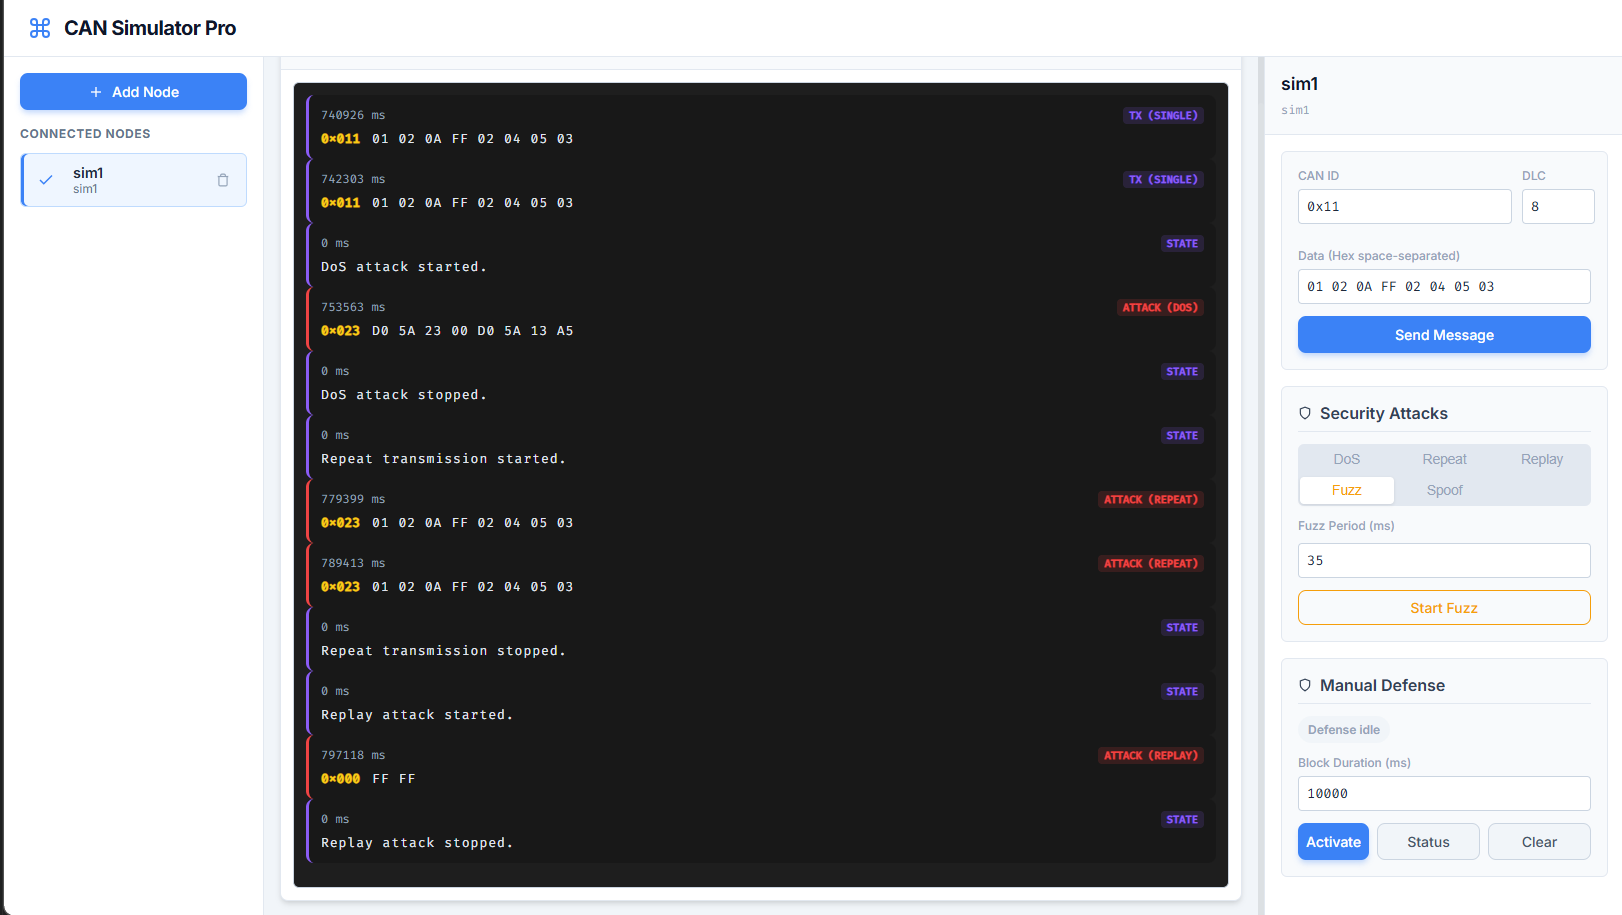
\includegraphics[width=0.88\textwidth]{images/web-interface.jpg}
            \caption{Giao diện web giám sát, tấn công và phòng thủ CAN}
        \end{figure}
    }{%
        \placeholderfigure{%
            Ảnh chụp màn hình giao diện web: danh sách nút, log thời gian thực,
            các nút kích hoạt tấn công và phòng thủ.\\
            Đặt ảnh tại \texttt{report/images/web-interface.png} hoặc \texttt{.jpg}%
        }{Giao diện web giám sát, tấn công và phòng thủ CAN}
    }%
}

% ----------------------------------------------------------
\reportsubsection{5.2.6 Quản lý trạng thái và lưu trữ dữ liệu}
% ----------------------------------------------------------

Hệ thống không sử dụng cơ sở dữ liệu lưu trữ bền vững. Phía firmware, toàn bộ
trạng thái vận hành được lưu trong bộ nhớ RAM nội bộ của ESP32, bao gồm khung bắt
gần nhất, bản ghi cảnh báo, các tác vụ tấn công đang chạy và bộ nhớ phòng thủ.
Dung lượng sử dụng nằm trong giới hạn an toàn của ESP32 với 520 kB SRAM tích hợp.

Phía ứng dụng web, trạng thái của tất cả nút và lịch sử khung quan sát được cũng
chỉ lưu trong bộ nhớ của tiến trình Python. Khi chương trình dừng, toàn bộ thông
tin này bị giải phóng. Thiết kế này phù hợp với mục tiêu trình diễn và thực nghiệm
ngắn hạn, nhưng cần bổ sung lớp lưu trữ bền vững nếu mở rộng sang các ứng dụng
giám sát dài hạn.

% ============================================================
\reportsection{5.3 Nguyên lý hoạt động của hệ thống}
% ============================================================

% ```mermaid
% flowchart TD
%     s1[Người dùng nhập lệnh terminal UART hoặc giao diện web]
%     s2[Kiểm tra ID, DLC và bổ sung byte số thứ tự]
% ```mermaid
% flowchart LR
%     s1("Nhập lệnh") --> s2("Chuẩn hóa") --> s3("Phát ra Bus")
%     s3 --> s4("Đọc từ Bus")
%     s4 --> d1{"Bị chặn?"}
%     
%     d1 -- "Có" --> drop("Loại bỏ")
%     d1 -- "Không" --> s5("Phân tích IDS")
%     
%     s5 -- "Phát hiện" --> alert("Sinh cảnh báo")
%     s5 -- "Bình thường" --> s6("Ghi log") --> s7("Cập nhật Web")
% ```
    \begin{figure}[H]
        \centering
        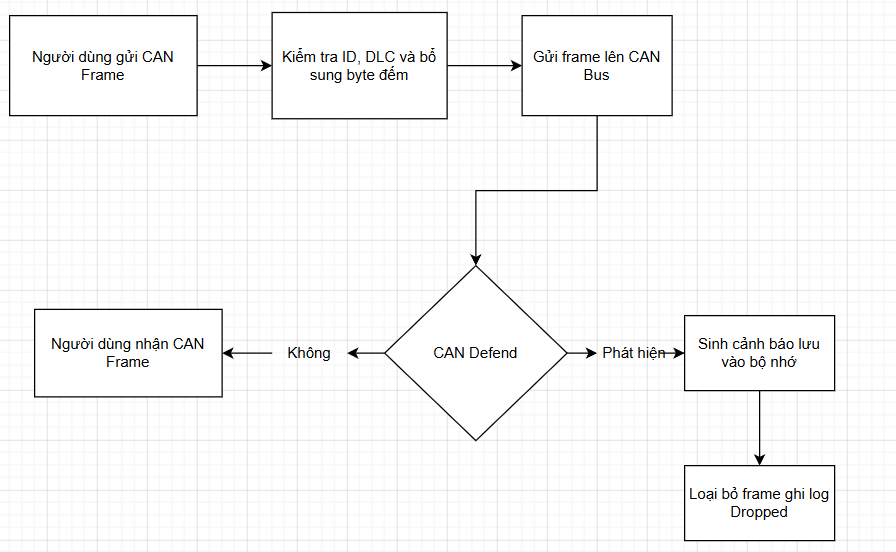
\includegraphics[width=0.75\textwidth]{images/so-do-luong-xu-ly.png}
        \caption{Sơ đồ luồng xử lý tổng thể của hệ thống}
    \end{figure}
%---------------------------------------------------------
\reportsubsection{5.3.1 Giao tiếp CAN cơ bản}
% ----------------------------------------------------------

Ở chế độ bình thường, người dùng gửi một khung CAN đơn bằng lệnh
\texttt{send <id> <dlc> <data>} qua terminal. Firmware kiểm tra tính hợp lệ của
các tham số, bổ sung byte số thứ tự vào cuối payload rồi phát lên bus. Khi nhận
được khung từ bus, nút ghi log theo định dạng chuẩn có nhãn thời gian, chiều
truyền, CAN ID, độ dài dữ liệu và nội dung. Đồng thời khung được lưu lại làm dữ
liệu nền cho tính năng phát lại. LED trên bo mạch nhấp nháy ngắn để xác nhận mỗi
sự kiện truyền hoặc nhận thành công.

% ----------------------------------------------------------
\reportsubsection{5.3.2 Cơ chế bảo vệ bộ đếm thông điệp}
% ----------------------------------------------------------

Khi tính năng bảo vệ bộ đếm được bật, mỗi khung gửi đi đều có thêm một byte số
thứ tự tăng dần ở vị trí byte cuối cùng của payload, làm tổng độ dài tăng lên một
byte. Bộ đếm là số nguyên 8-bit không dấu, tăng liên tục và quay về 0 sau giá trị
255. Phía nhận đọc byte cuối của mỗi khung đến, đối chiếu với giá trị kỳ vọng dựa
trên lần nhận trước của cùng CAN ID. Bất kỳ sai lệch nào đều bị ghi nhận là dấu
hiệu bất thường và sinh cảnh báo phát lại loại đếm ngược.

% ----------------------------------------------------------
\reportsubsection{5.3.3 Replay Attack}
% ----------------------------------------------------------

\begin{itemize}[leftmargin=*]
    \item \textbf{Mô hình tấn công:} Tấn công phát lại (Replay Attack) xảy ra khi một thực thể trái phép tiến hành rình rập (sniffing) và sao chép các thông điệp CAN hợp lệ đang truyền tải trên bus. Sau đó, thực thể này tái phát (inject) các thông điệp nguyên bản đó vào mạng tại một thời điểm khác.
    \item \textbf{Hậu quả:} Các Bộ điều khiển điện tử (ECU) sẽ tiếp nhận và thực thi các lệnh bị lặp lại (ví dụ: kích hoạt hệ thống phanh, vô hiệu hóa khóa cửa) do giao thức CAN nguyên thủy thiếu vẹn toàn về nhãn thời gian. Điều này dẫn đến sự sai lệch nghiêm trọng trong trạng thái vận hành của phương tiện.
    \item \textbf{Cơ chế phòng thủ:} Giải pháp lý thuyết tối ưu để ngăn chặn tấn công phát lại là tích hợp các định danh động như bộ đếm tăng dần (Monotonic Counter) hoặc Mã xác thực thông điệp (MAC) vào dữ liệu tải. Qua đó, hệ thống phát hiện xâm nhập (IDS) có thể kiểm chứng tính mới (freshness) của dữ liệu và loại bỏ các gói tin lỗi thời.
\end{itemize}



% ----------------------------------------------------------
\reportsubsection{5.3.4 Spoofing Attack}
% ----------------------------------------------------------

\begin{itemize}[leftmargin=*]
    \item \textbf{Mô hình tấn công:} Tấn công giả mạo (Spoofing) là kỹ thuật đánh lừa định tuyến, trong đó kẻ tấn công phát đi các khung dữ liệu mang CAN ID hợp lệ nhưng cố ý ngụy tạo cấu trúc hoặc giá trị của vùng dữ liệu tải (payload) nhằm đánh lừa các ECU đích.
    \item \textbf{Hậu quả:} Việc tiêm các thông số giả mạo (ví dụ: tốc độ vòng tua động cơ, nhiệt độ cảm biến) sẽ làm nhiễu loạn logic điều khiển của hệ thống. Nếu các ECU đưa ra quyết định dựa trên luồng dữ liệu giả mạo này, sự an toàn cơ học của phương tiện có thể bị đe dọa trực tiếp.
    \item \textbf{Cơ chế phòng thủ:} Phương thức phòng vệ nền tảng là xây dựng mô hình hành vi bình thường (baseline) cho mạng CAN dựa trên chu kỳ phát và đặc trưng tải trọng của từng định danh. Mọi sự sai lệch bất thường về độ dài dữ liệu (DLC) hoặc giá trị payload lệch khỏi quỹ đạo thống kê đều bị IDS phân loại là hành vi giả mạo.
\end{itemize}

% ----------------------------------------------------------
\reportsubsection{5.3.5 DoS Attack}
% ----------------------------------------------------------

\begin{itemize}[leftmargin=*]
    \item \textbf{Mô hình tấn công:} Tấn công từ chối dịch vụ (Denial of Service - DoS) được thực thi thông qua việc bơm tràn ngập (flooding) mạng CAN bằng các khung dữ liệu mang định danh có mức độ ưu tiên cao nhất (CAN ID mang giá trị thấp) với tần suất cực đại.
    \item \textbf{Hậu quả:} Do cơ chế phân xử tranh chấp dựa trên mức ưu tiên (Arbitration) của giao thức CAN, các thông điệp từ các ECU hợp lệ sẽ liên tục bị từ chối quyền truy cập bus. Trạng thái này gây ra độ trễ nghiêm trọng hoặc làm tê liệt hoàn toàn khả năng trao đổi thông tin của toàn mạng.
    \item \textbf{Cơ chế phòng thủ:} Cơ sở lý luận để giảm thiểu DoS là giám sát và phân tích lưu lượng dựa trên tần suất (Rate-based Intrusion Detection). Hệ thống IDS cần tính toán mật độ thông điệp trong các cửa sổ thời gian (time windows). Bất cứ nút nào phát sinh lưu lượng vượt quá giới hạn băng thông lý thuyết của mạng sẽ bị nhận diện và cách ly.
\end{itemize}



% ----------------------------------------------------------
\reportsubsection{5.3.6 Fuzzing Attack}
% ----------------------------------------------------------

\begin{itemize}[leftmargin=*]
    \item \textbf{Mô hình tấn công:} Quét ngẫu nhiên (Fuzzing) là chiến lược tấn công diện rộng, trong đó kẻ tấn công liên tục tiêm vào bus hàng loạt khung CAN với các định danh (ID) và vùng dữ liệu tải (payload) được sinh ngẫu nhiên hoàn toàn sau mỗi chu kỳ.
    \item \textbf{Hậu quả:} Cuộc tấn công này đẩy các ECU vào trạng thái phải liên tục xử lý một khối lượng khổng lồ các thông điệp rác không xác định. Việc này không chỉ gây lãng phí tài nguyên xử lý mà còn có thể vô tình kích hoạt các chức năng ẩn (diagnostic messages), dẫn đến hệ thống hoạt động hỗn loạn.
    \item \textbf{Cơ chế phòng thủ:} Khác với việc giám sát theo từng ID đơn lẻ, nguyên lý nhận diện Fuzzing dựa trên phép phân tích tính biến động toàn cục của bus. Sự xuất hiện ồ ạt của các ID ngoại lai hoặc tỷ lệ luân chuyển ID quá cao trong một đơn vị thời gian là các đặc trưng dị thường giúp IDS kích hoạt trạng thái phòng vệ.
\end{itemize}



% ----------------------------------------------------------
\reportsubsection{5.3.7 Cơ chế phòng thủ chủ động}
% ----------------------------------------------------------

Sau khi IDS phát sinh cảnh báo, người vận hành có thể kích hoạt phòng thủ qua lệnh
terminal hoặc nút tương ứng trên giao diện web. Hệ thống đọc thông tin từ cảnh báo
gần nhất và thiết lập quy tắc chặn phù hợp với từng loại tấn công. Thời gian
duy trì luật chặn mặc định là 10 giây nhưng có thể tùy chỉnh.

\begin{table}[H]
\centering
\begin{tabular}{|>{\raggedright\arraybackslash}p{3.2cm}|>{\raggedright\arraybackslash}p{4.0cm}|>{\raggedright\arraybackslash}p{6.2cm}|}
\hline
\textbf{Loại tấn công} & \textbf{Đối tượng bị chặn} & \textbf{Tiêu chí lọc} \\ \hline
Replay (phát lại) & Khung cùng ID và nội dung & Khớp chính xác với chữ ký khung bị cảnh báo \\ \hline
DoS (ngập lưu lượng) & Mọi khung cùng ID & Chặn toàn bộ, không phân biệt nội dung \\ \hline
Spoofing (giả mạo) & Khung cùng ID đáng ngờ & Lọc theo độ lệch so với baseline đã học \\ \hline
Fuzzing (quét ngẫu nhiên) & Mọi ID chưa tin cậy & Chỉ cho phép ID đã ổn định trước cảnh báo \\ \hline
\end{tabular}
\caption{Chiến lược phòng thủ theo từng loại tấn công}
\end{table}

Cần lưu ý rằng cơ chế phòng thủ hiện tại hoạt động ở tầng phần mềm của nút nhận,
không loại bỏ khung tấn công khỏi bus vật lý. Kẻ tấn công vẫn có thể tiếp tục phát
khung; hệ thống chỉ ngăn tầng ứng dụng xử lý các khung bị nghi ngờ trong thời gian
áp dụng luật chặn. Đây là hạn chế vốn có của kiến trúc CAN không có cơ chế xác thực ở lớp
liên kết dữ liệu và là hướng mở rộng tiếp theo của đề tài.

\chapter{Thực thi, đo lường và đánh giá}

\reportsection{I. Giao tiếp 2 chiều}

Trong giai đoạn giao tiếp 2 chiều, hệ thống được vận hành với hai nút ESP32 tham gia
cùng một bus CAN để kiểm tra khả năng gửi và nhận bản tin theo cả hai chiều. Mục tiêu
của phần này là chứng minh rằng mô hình phần cứng và firmware hiện tại có thể duy trì
trao đổi dữ liệu ổn định trước khi đưa thêm các kịch bản tấn công và cơ chế phòng thủ.

\IfFileExists{images/mach_2_node.png}{%
\begin{figure}[H]
  \centering
  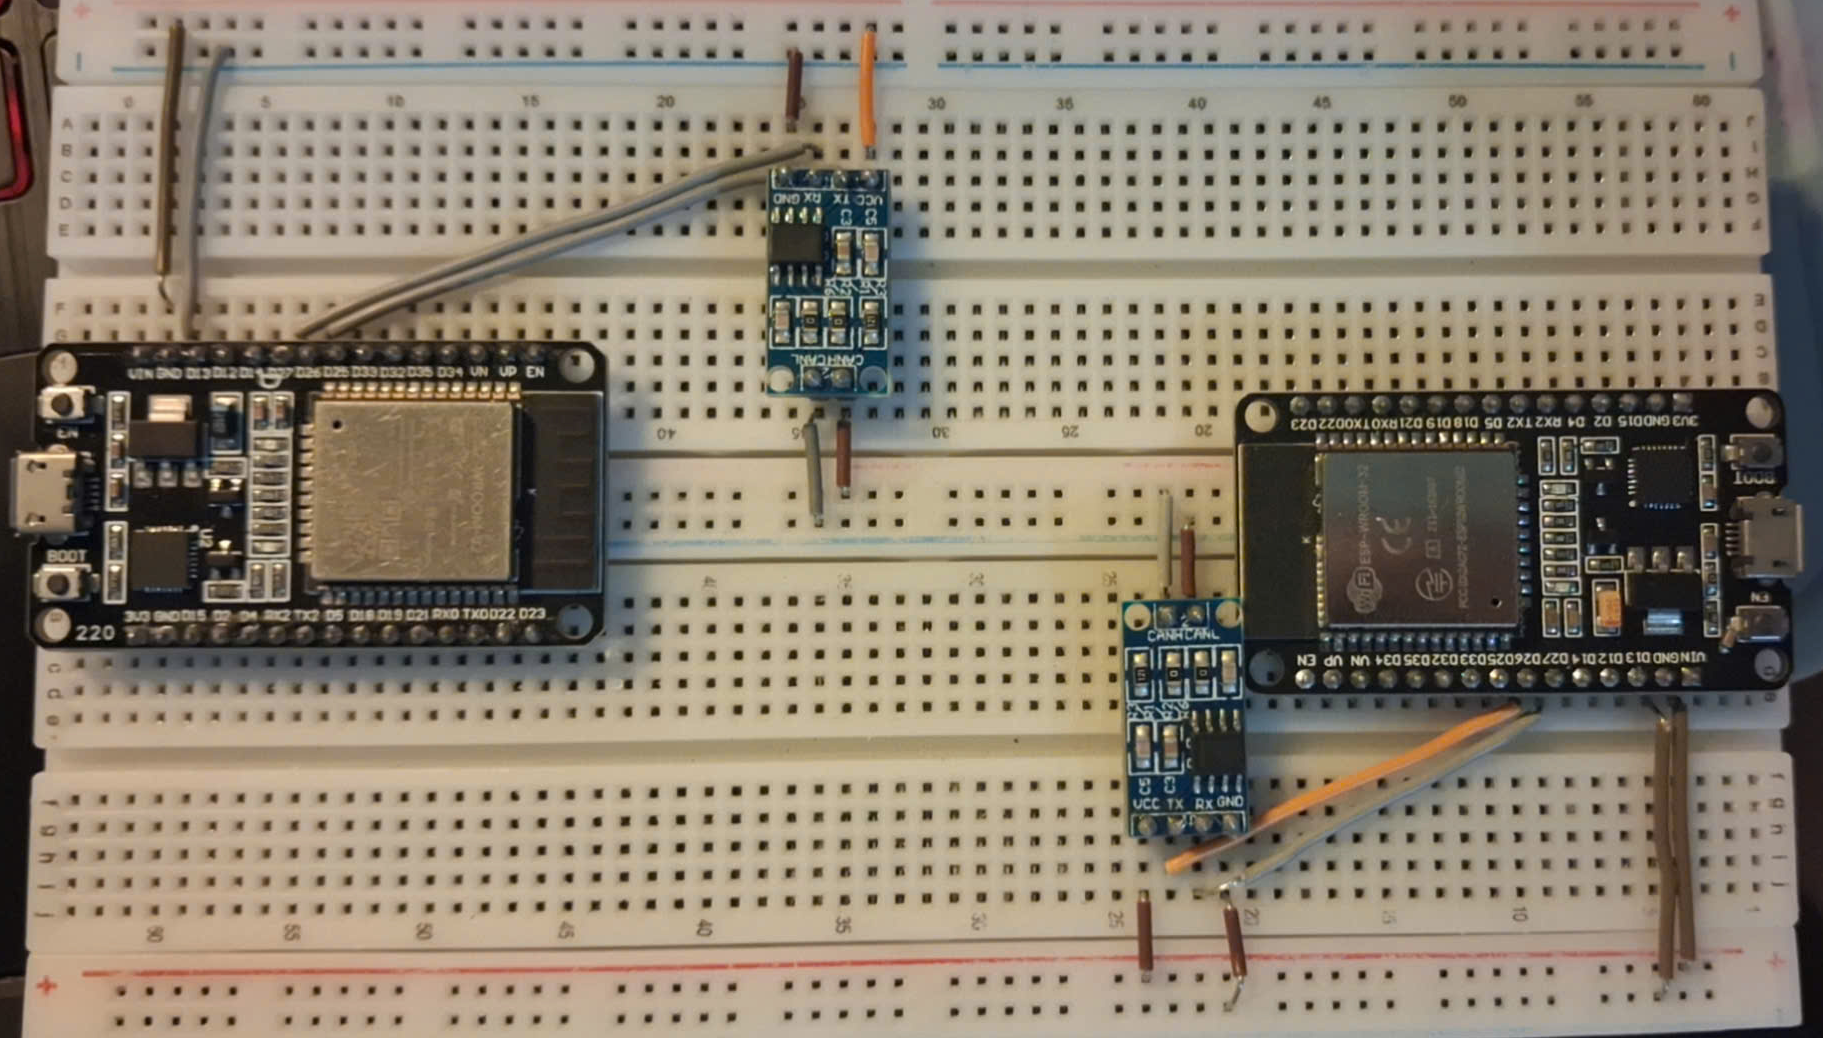
\includegraphics[width=0.62\textwidth]{images/mach_2_node.png}
  \caption{Mô hình phần cứng giao tiếp CAN với 2 node ESP32}
  \label{fig:mach-2-node}
\end{figure}
}{%
\placeholderfigure{Ảnh mạch thực tế khi hệ thống chỉ gồm 2 node ESP32 giao tiếp qua CAN}{Mô
hình phần cứng giao tiếp CAN với 2 node ESP32}
}

\IfFileExists{images/ch6-can-two-way-web.png}{%
\begin{figure}[H]
  \centering
  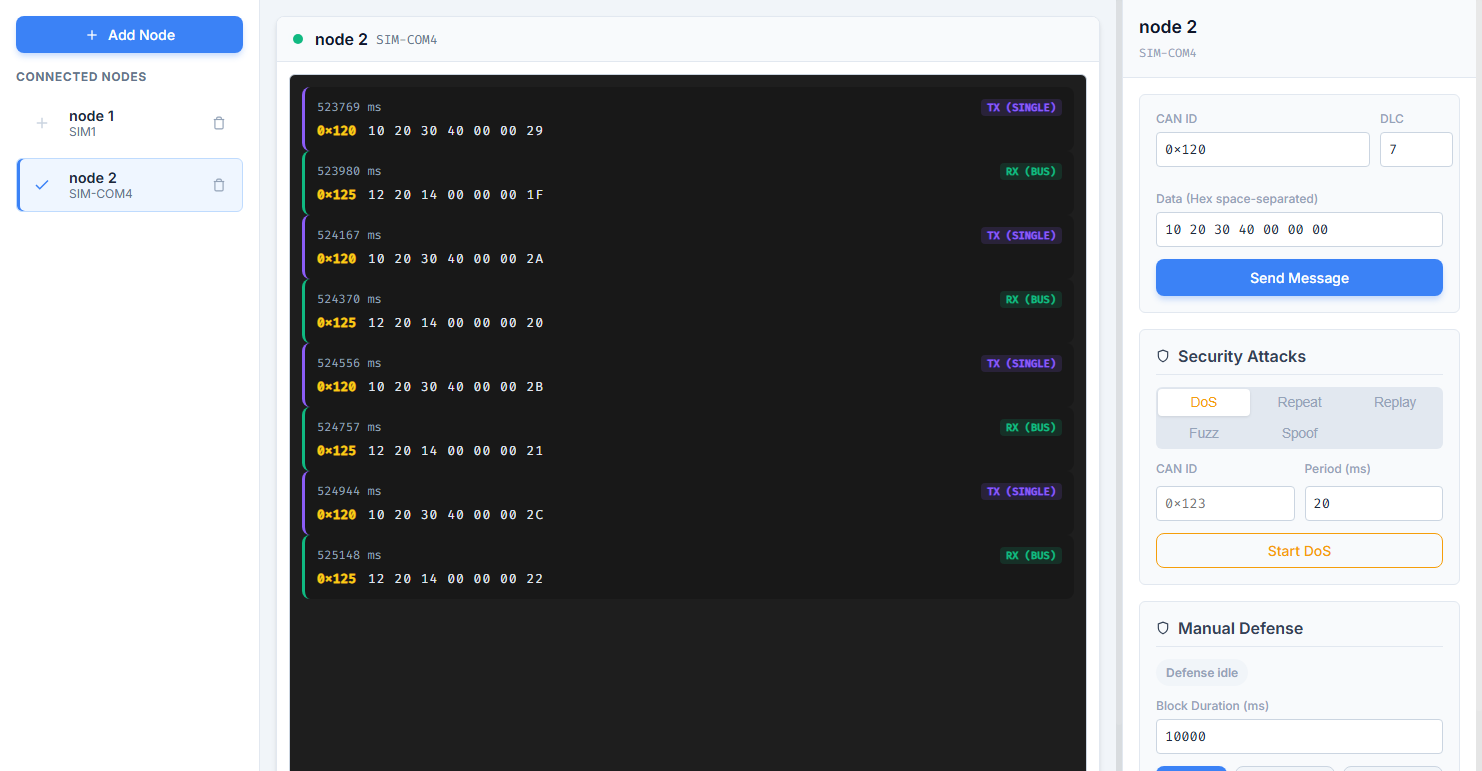
\includegraphics[width=0.98\textwidth]{images/ch6-can-two-way-web.png}
  \caption{Phiên giao tiếp CAN hai chiều bình thường hiển thị trên giao diện web}
  \label{fig:can-two-way-web}
\end{figure}
}

Ảnh chụp ở Hình \ref{fig:can-two-way-web} cho thấy nút \texttt{node 2} vừa phát khung CAN
ID \texttt{0x120} vừa nhận khung ID \texttt{0x125} từ nút còn lại trên cùng bus. Các bản tin TX
và RX xuất hiện xen kẽ, đồng thời byte cuối của dữ liệu thay đổi tuần tự theo từng lần gửi.

\reportsection{II. Các kịch bản tấn công và phản ứng phòng thủ}

Để mô phỏng tấn công trên mạng CAN, hệ thống bổ sung thêm một nút thứ ba đóng vai trò
thiết bị tấn công. Nút này có nhiệm vụ quan sát lưu lượng hợp lệ trên bus, lưu lại bản tin đã
thu được và phát lại hoặc phát dồn với chu kỳ xác định nhằm kiểm tra khả năng chịu lỗi của
hệ thống truyền nhận.

\IfFileExists{images/mo-hinh-thuc-nghiem.png}{%
\begin{figure}[H]
  \centering
  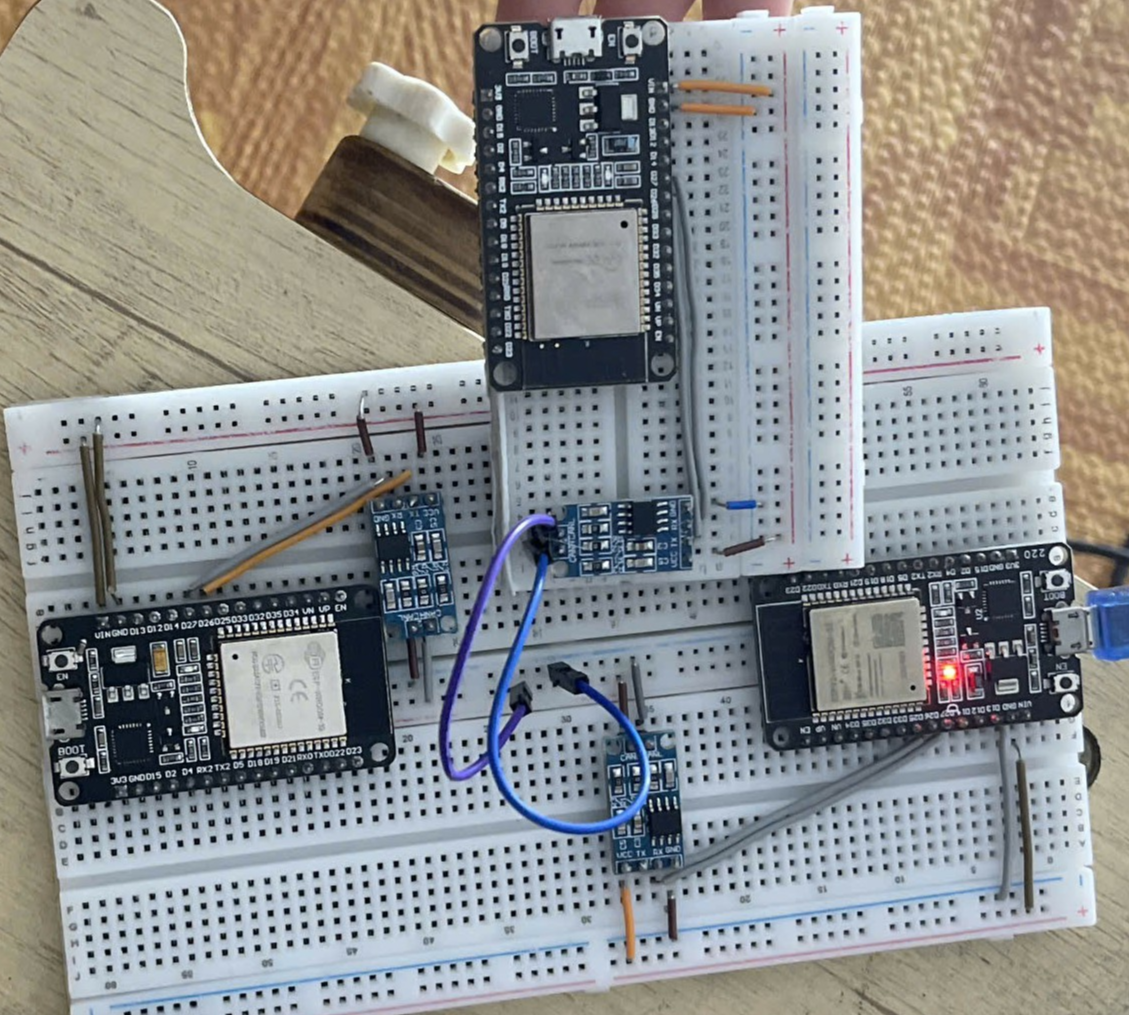
\includegraphics[width=0.72\textwidth]{images/mo-hinh-thuc-nghiem.png}
  \caption{Mô hình phần cứng thực tế khi bổ sung thêm node hacker vào bus CAN}
  \label{fig:mach-hacker}
\end{figure}
}{%
\placeholderfigure{Ảnh mô hình phần cứng khi bổ sung thêm nút tấn công vào bus CAN}{Mạch
giao tiếp CAN thêm phần tử Hacker}
}

Trên giao diện điều khiển, người vận hành có thể chọn nút đang thao tác, cấu hình tham số
tấn công và theo dõi phản hồi của từng nút theo thời gian thực. Để phần đánh giá rõ ràng
hơn, chương này trình bày theo từng kịch bản riêng gồm DoS, Replay, Fuzzing và Spoofing.
Trong mỗi kịch bản, kết quả được mô tả theo hai bước liên tiếp: bước hệ thống sinh cảnh báo
\texttt{ALERT} và bước người vận hành kích hoạt \texttt{defense} để chặn hoặc giảm tác động
của lưu lượng bất thường lên nút nhận.

\reportsubsection{1. Tấn công DoS}

Trong kịch bản DoS, nút tấn công phát liên tiếp nhiều khung CAN cùng một ID với chu kỳ rất
ngắn để làm tăng nhanh mật độ lưu lượng trên bus. Mục tiêu của phần này là kiểm tra khả
năng quan sát hiện tượng ngập bản tin ở nút nhận và khả năng sinh cảnh báo khi tốc độ khung
vượt ngưỡng bình thường.

\IfFileExists{images/dos_alert.png}{%
\begin{figure}[H]
  \centering
  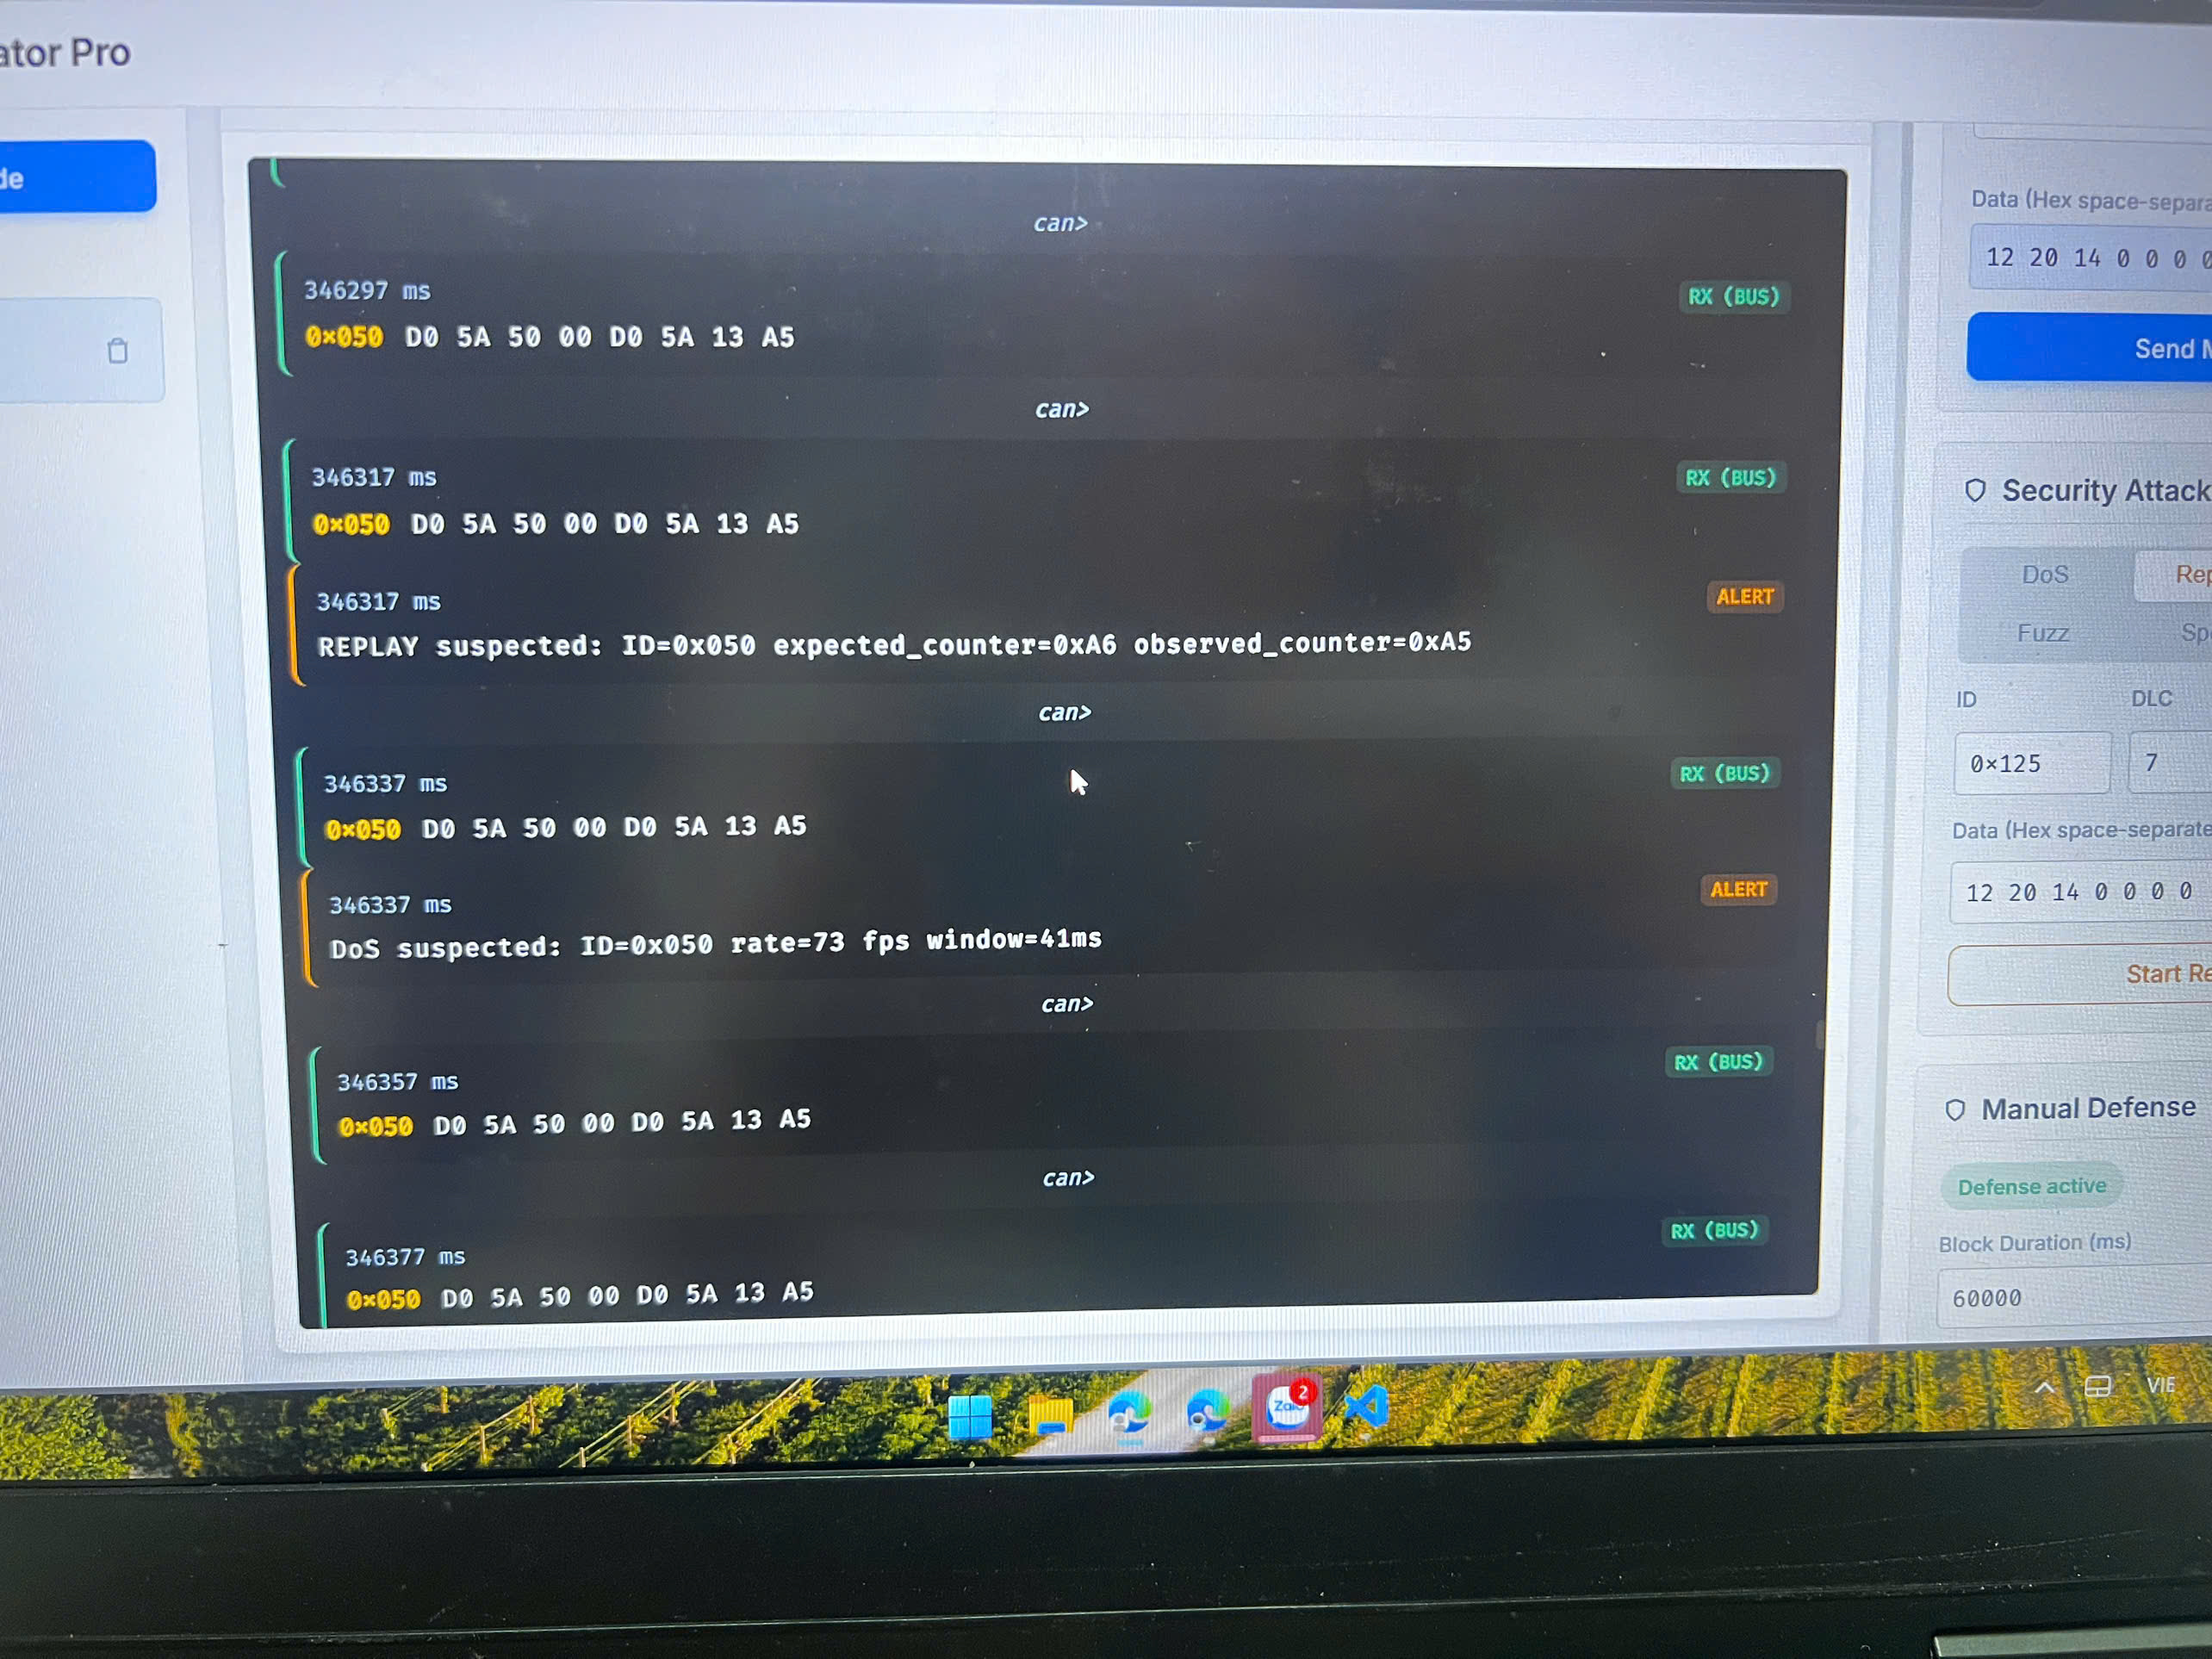
\includegraphics[width=0.98\textwidth]{images/dos_alert.png}
  \caption{Giao diện ghi nhận cảnh báo ở giai đoạn phát hiện tấn công DoS}
  \label{fig:dos-alert}
\end{figure}
}{%
\placeholderfigure{Ảnh giao diện web khi xuất hiện cảnh báo DoS suspected trên nút nhận}{Giao
diện cảnh báo tấn công DoS}
}

Khi DoS diễn ra, giao diện phía nút nhận thường xuất hiện dày đặc các bản tin RX cùng ID,
trong khi phần cảnh báo có thể hiển thị trạng thái \texttt{DoS suspected}. Trên bus, hiện tượng
này tương ứng với việc số khung hợp lệ tăng mạnh trong một cửa sổ thời gian ngắn.

\textbf{Bước cảnh báo:} Ở Hình \ref{fig:dos-alert}, các khung RX với ID \texttt{0x050} xuất hiện
liên tiếp trên giao diện,
đồng thời hệ thống sinh ra nhãn \texttt{ALERT} với dòng \texttt{DoS suspected}. Điều này cho
thấy bộ phát hiện đã nhận ra tốc độ khung tăng bất thường và đánh dấu đây là một phiên có dấu
hiệu ngập lưu lượng. Trong ảnh còn có thêm một dòng \texttt{REPLAY suspected} xuất hiện
trước đó, nhưng trọng tâm của bước này là cảnh báo \texttt{DoS suspected} dùng để kích hoạt
cơ chế phòng thủ ở bước tiếp theo.

\IfFileExists{images/dos_defend.png}{%
\begin{figure}[H]
  \centering
  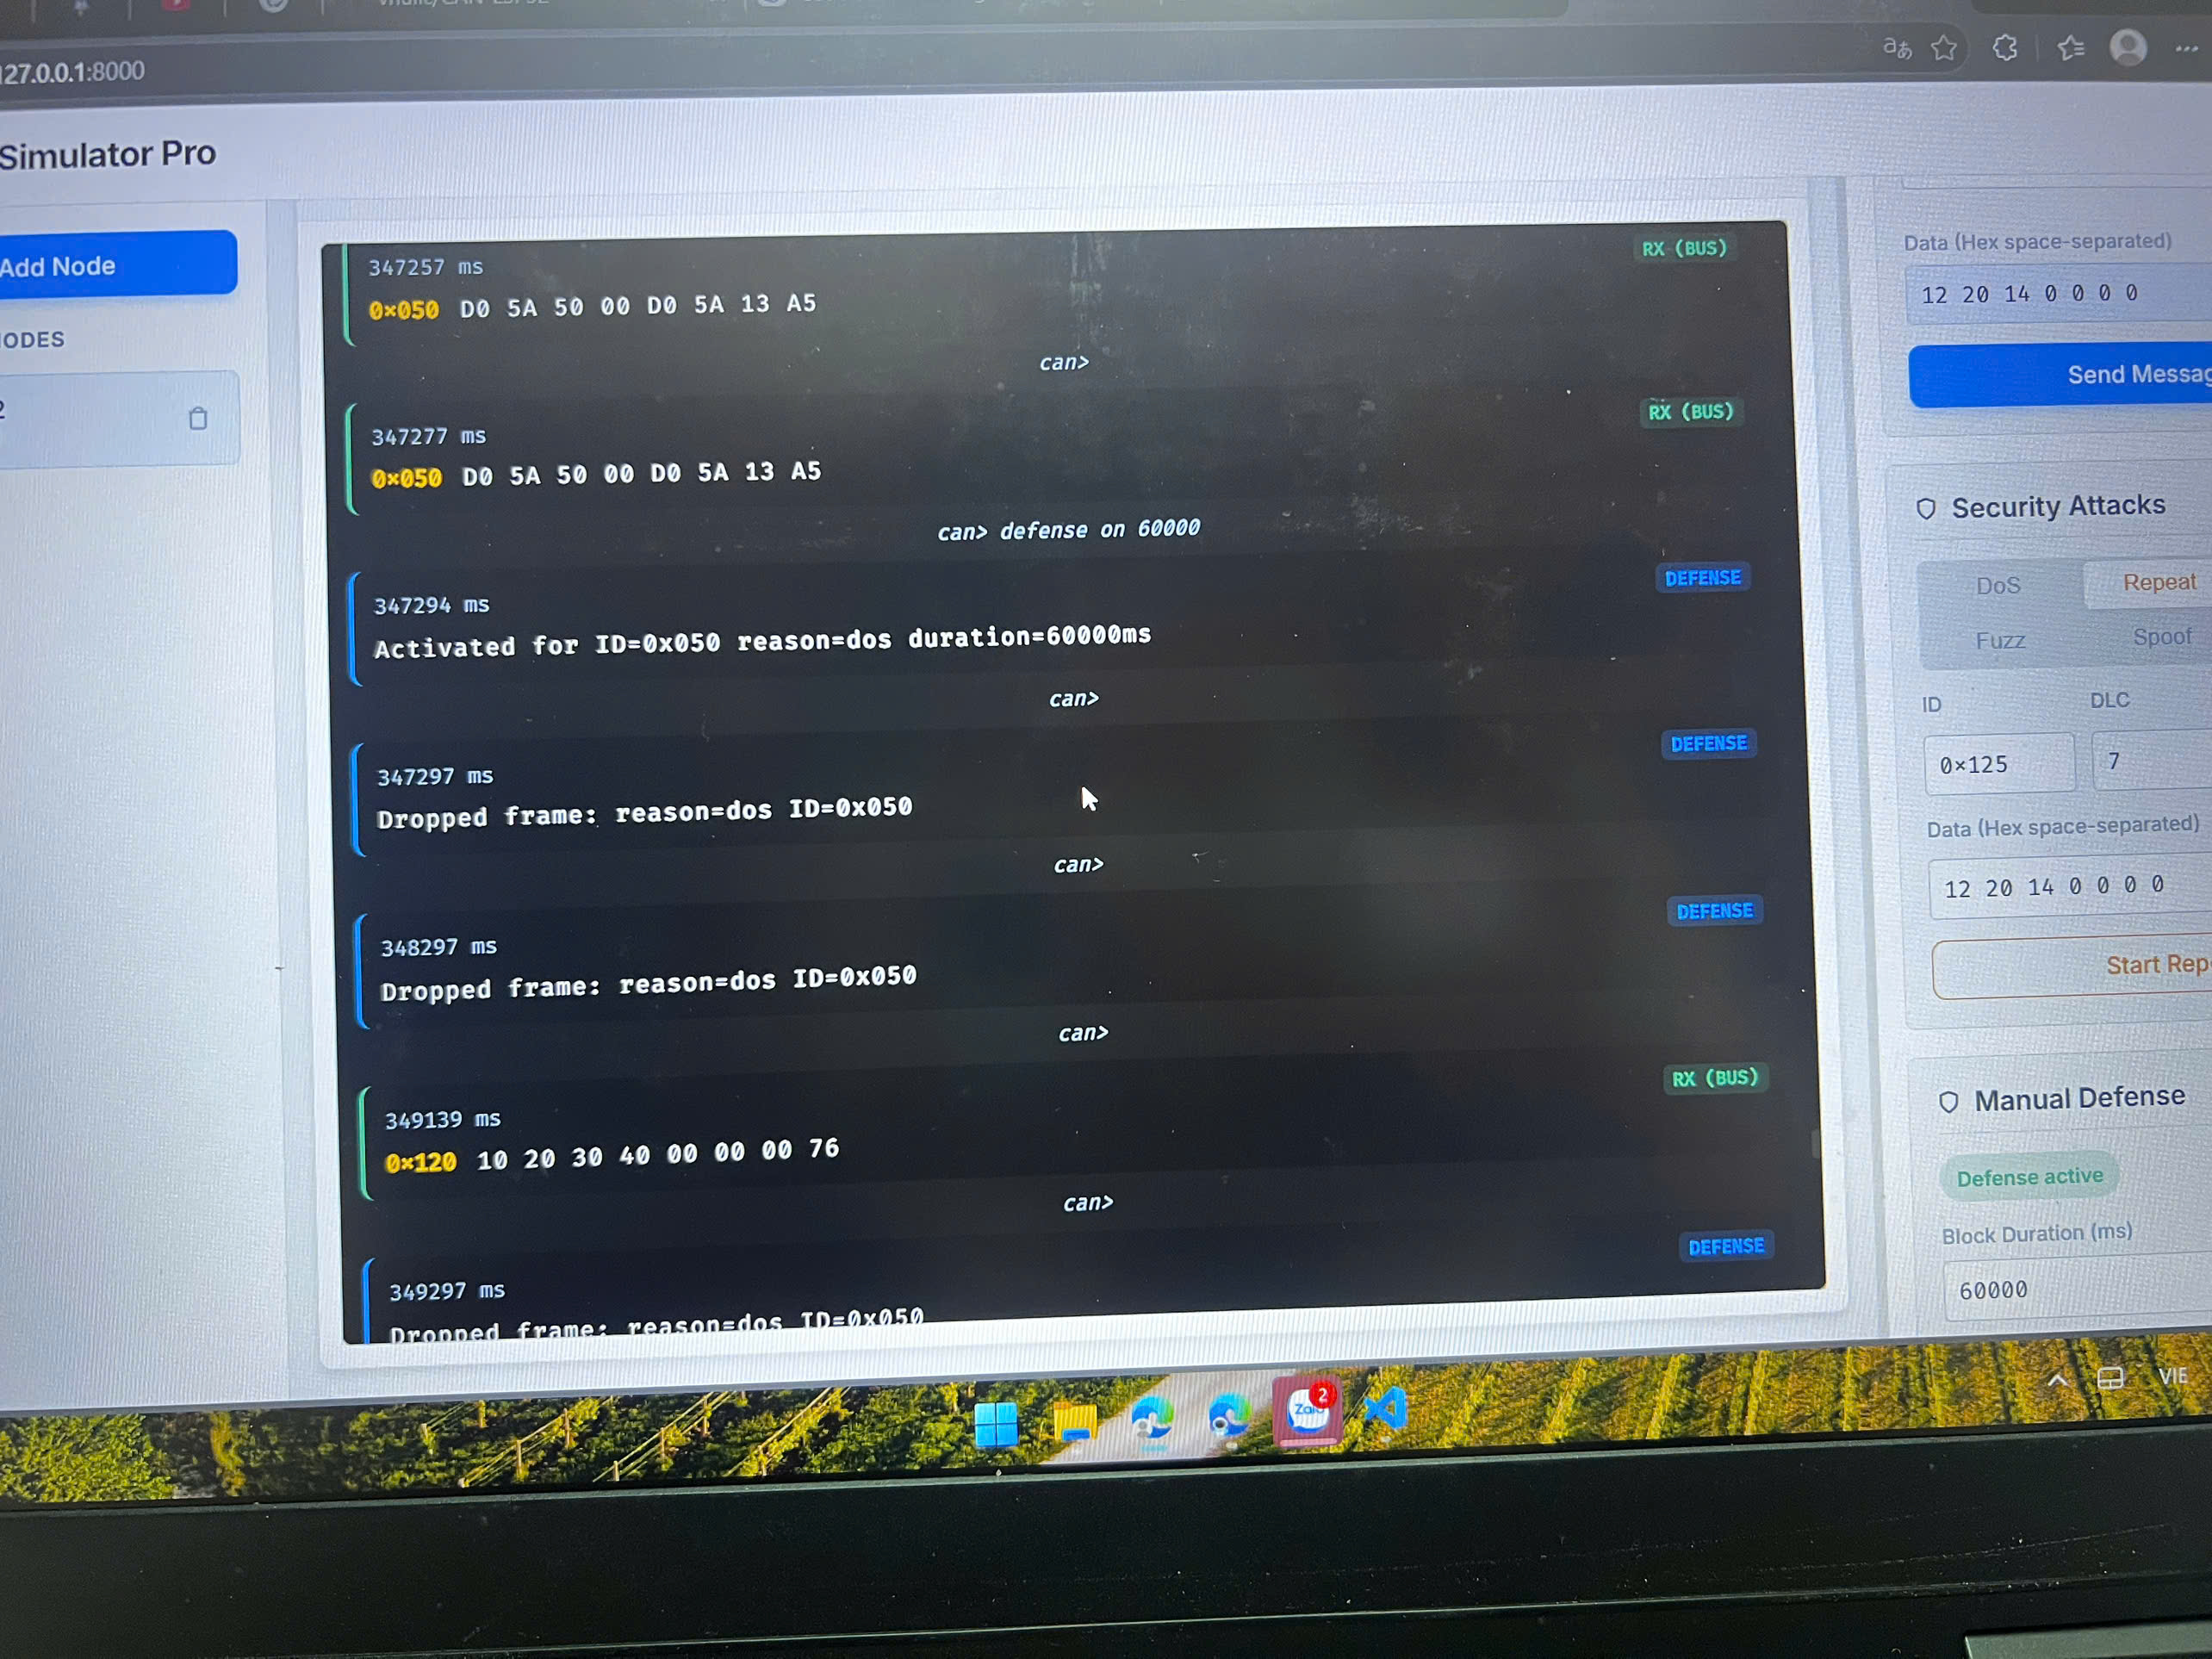
\includegraphics[width=0.98\textwidth]{images/dos_defend.png}
  \caption{Giao diện sau khi bật defense để chặn lưu lượng DoS}
  \label{fig:dos-defend}
\end{figure}
}{%
\placeholderfigure{Ảnh log hiển thị cảnh báo DoS và các khung bị chặn sau khi bật phòng thủ}{Phòng
thủ đối với kịch bản DoS}
}

\textbf{Bước phòng thủ:} Ở Hình \ref{fig:dos-defend}, sau khi người vận hành gửi lệnh
\texttt{defense on 60000}, hệ thống xác nhận kích hoạt phòng thủ bằng thông báo
\texttt{Activated for ID=0x050 reason=dos}. Ngay sau đó, các khung tiếp theo thuộc ID nghi
ngờ không còn được xử lý như dữ liệu hợp lệ mà bị ghi nhận dưới dạng \texttt{Dropped frame}.
Kết quả này cho thấy cơ chế \textit{defend} không làm mất hoàn toàn lưu lượng trên bus vật lý,
nhưng đã chặn được tác động của luồng DoS lên tầng ứng dụng ở nút nhận.

\reportsubsection{2. Tấn công Replay}

Kịch bản Replay yêu cầu nút tấn công đã quan sát được ít nhất một khung hợp lệ trên bus
trước khi phát lại. Sau khi lệnh \texttt{replay start} được kích hoạt, khung vừa thu sẽ được gửi
lặp theo chu kỳ định sẵn, nhằm kiểm tra khả năng phát hiện khung lặp của hệ thống.

\IfFileExists{images/replay_alert.png}{%
\begin{figure}[H]
  \centering
  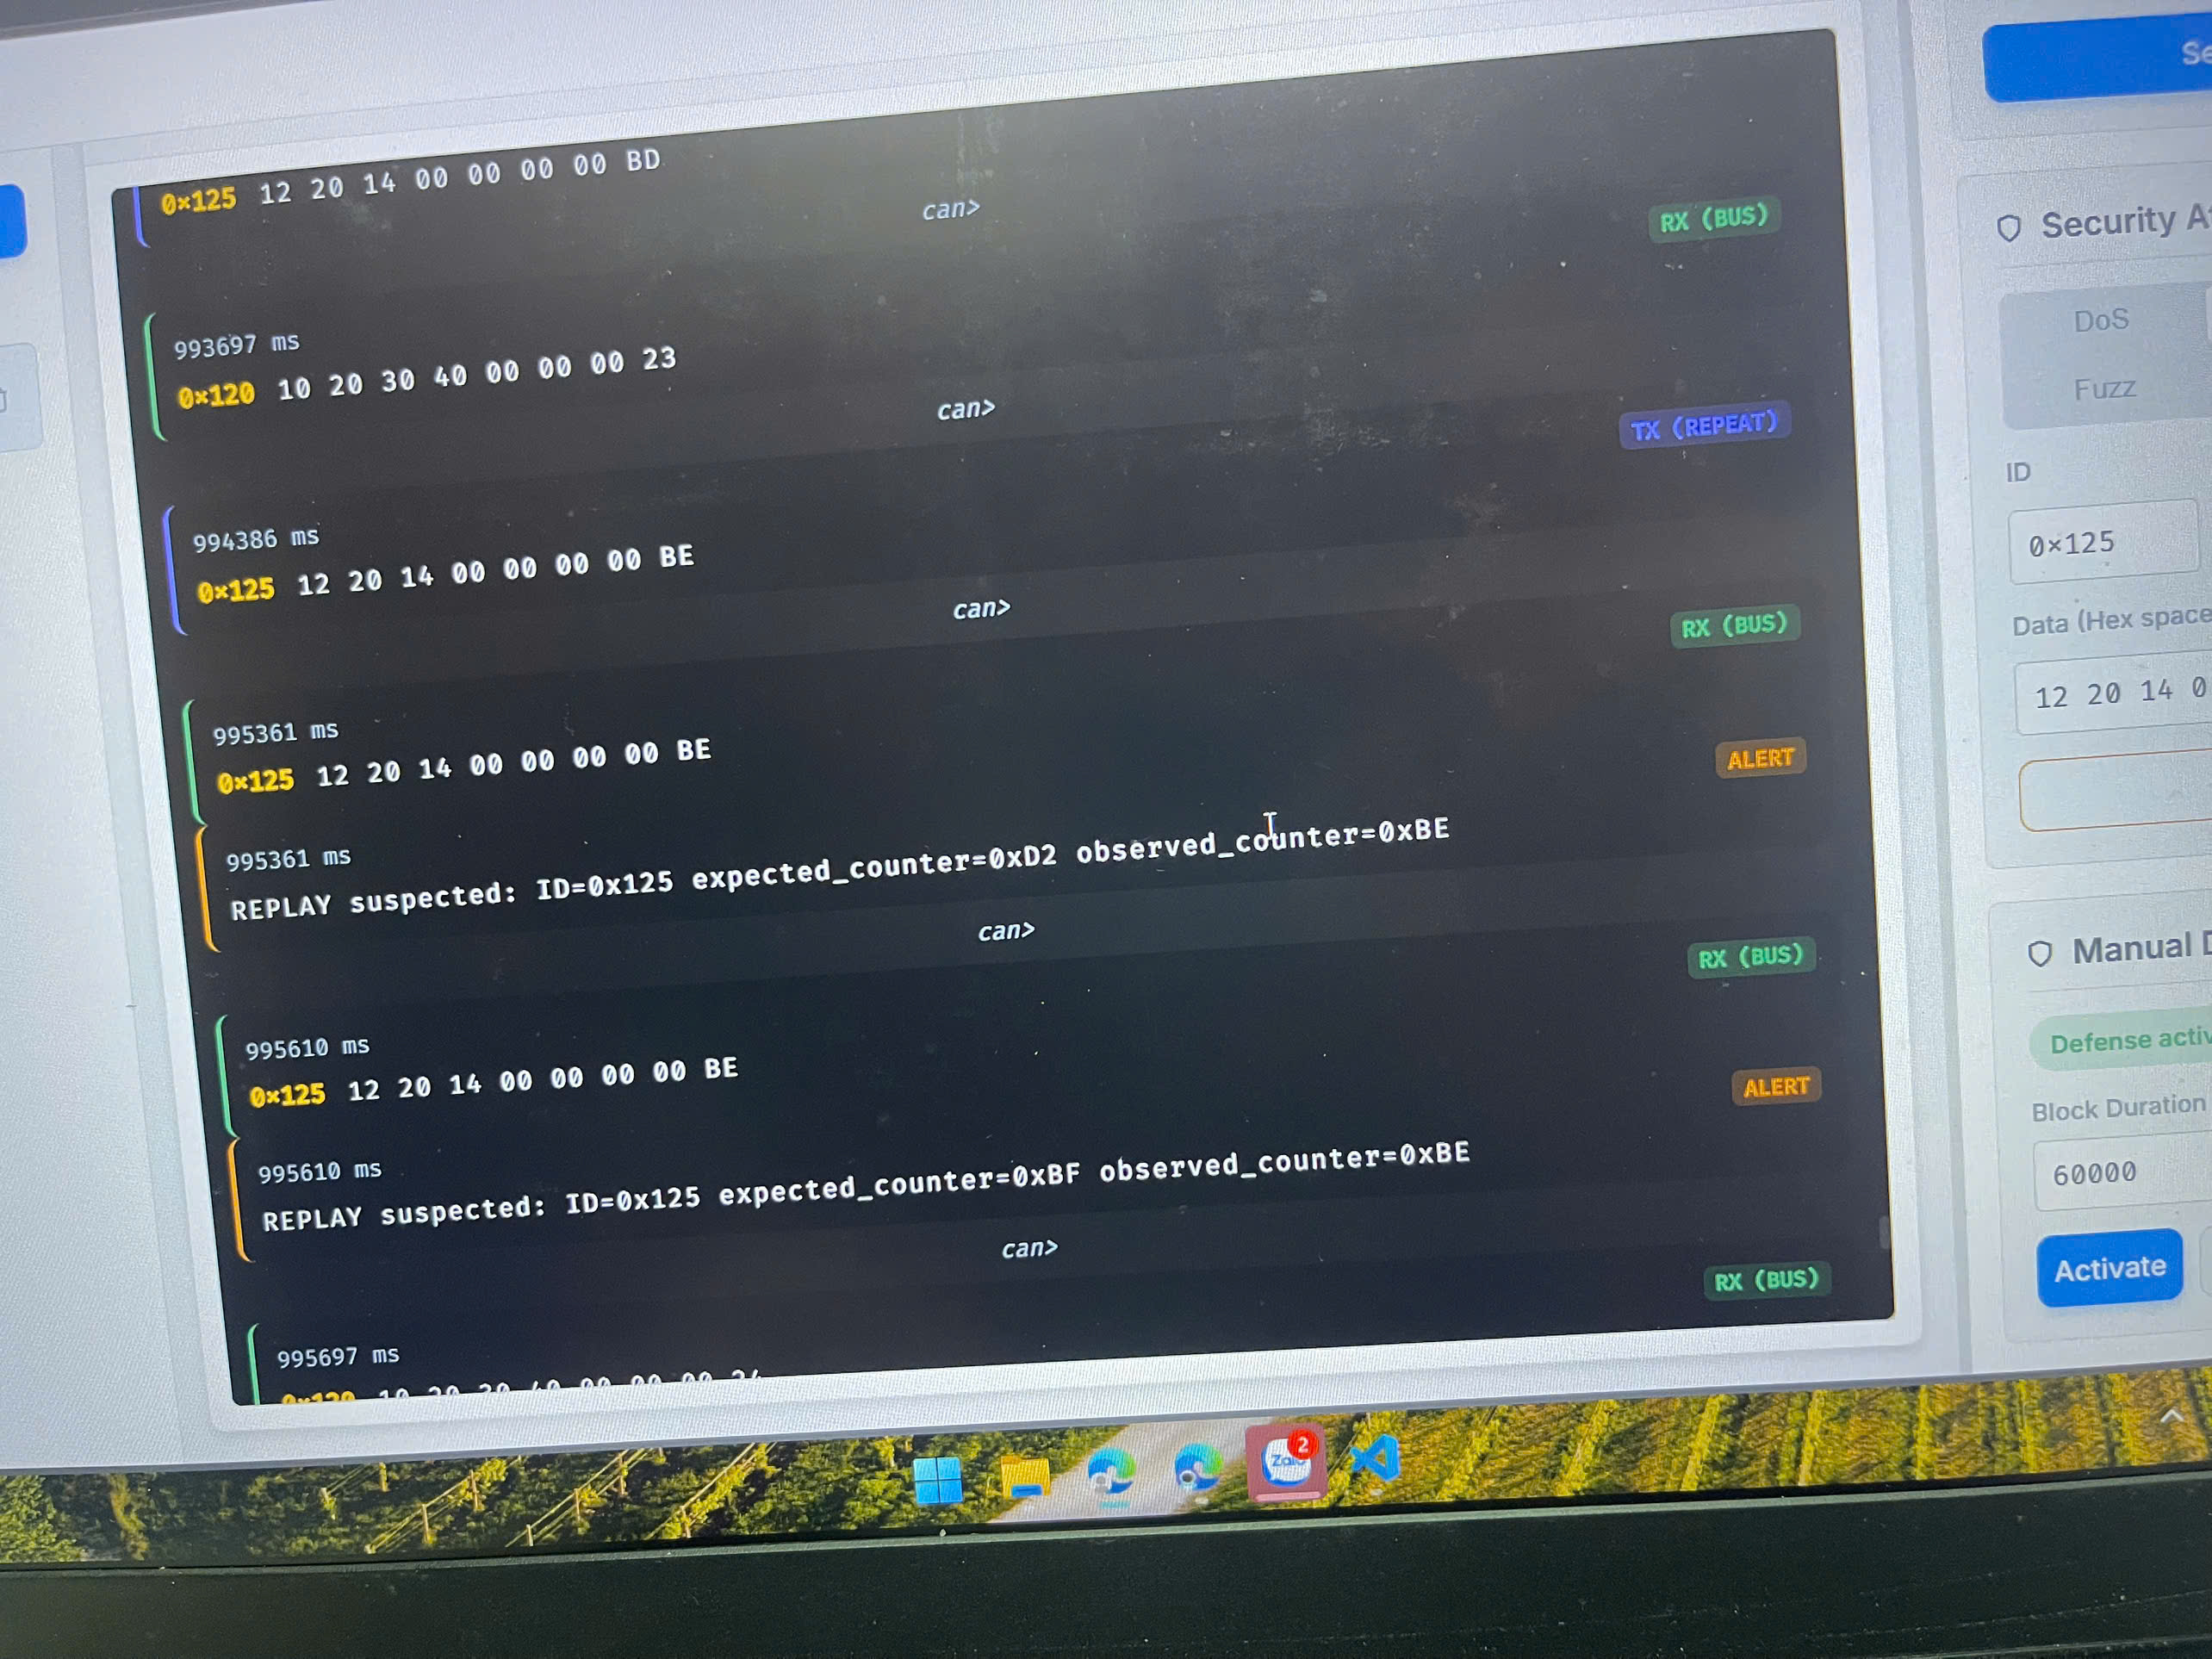
\includegraphics[width=0.9875\textwidth]{images/replay_alert.png}
  \caption{Giao diện ghi nhận cảnh báo ở giai đoạn phát hiện tấn công Replay}
  \label{fig:replay-alert}
\end{figure}
}{%
\placeholderfigure{Ảnh giao diện hoặc terminal khi xuất hiện cảnh báo replay trên nút nhận}{Cảnh
báo tấn công Replay}
}

\IfFileExists{images/replay_defend.png}{%
\begin{figure}[H]
  \centering
  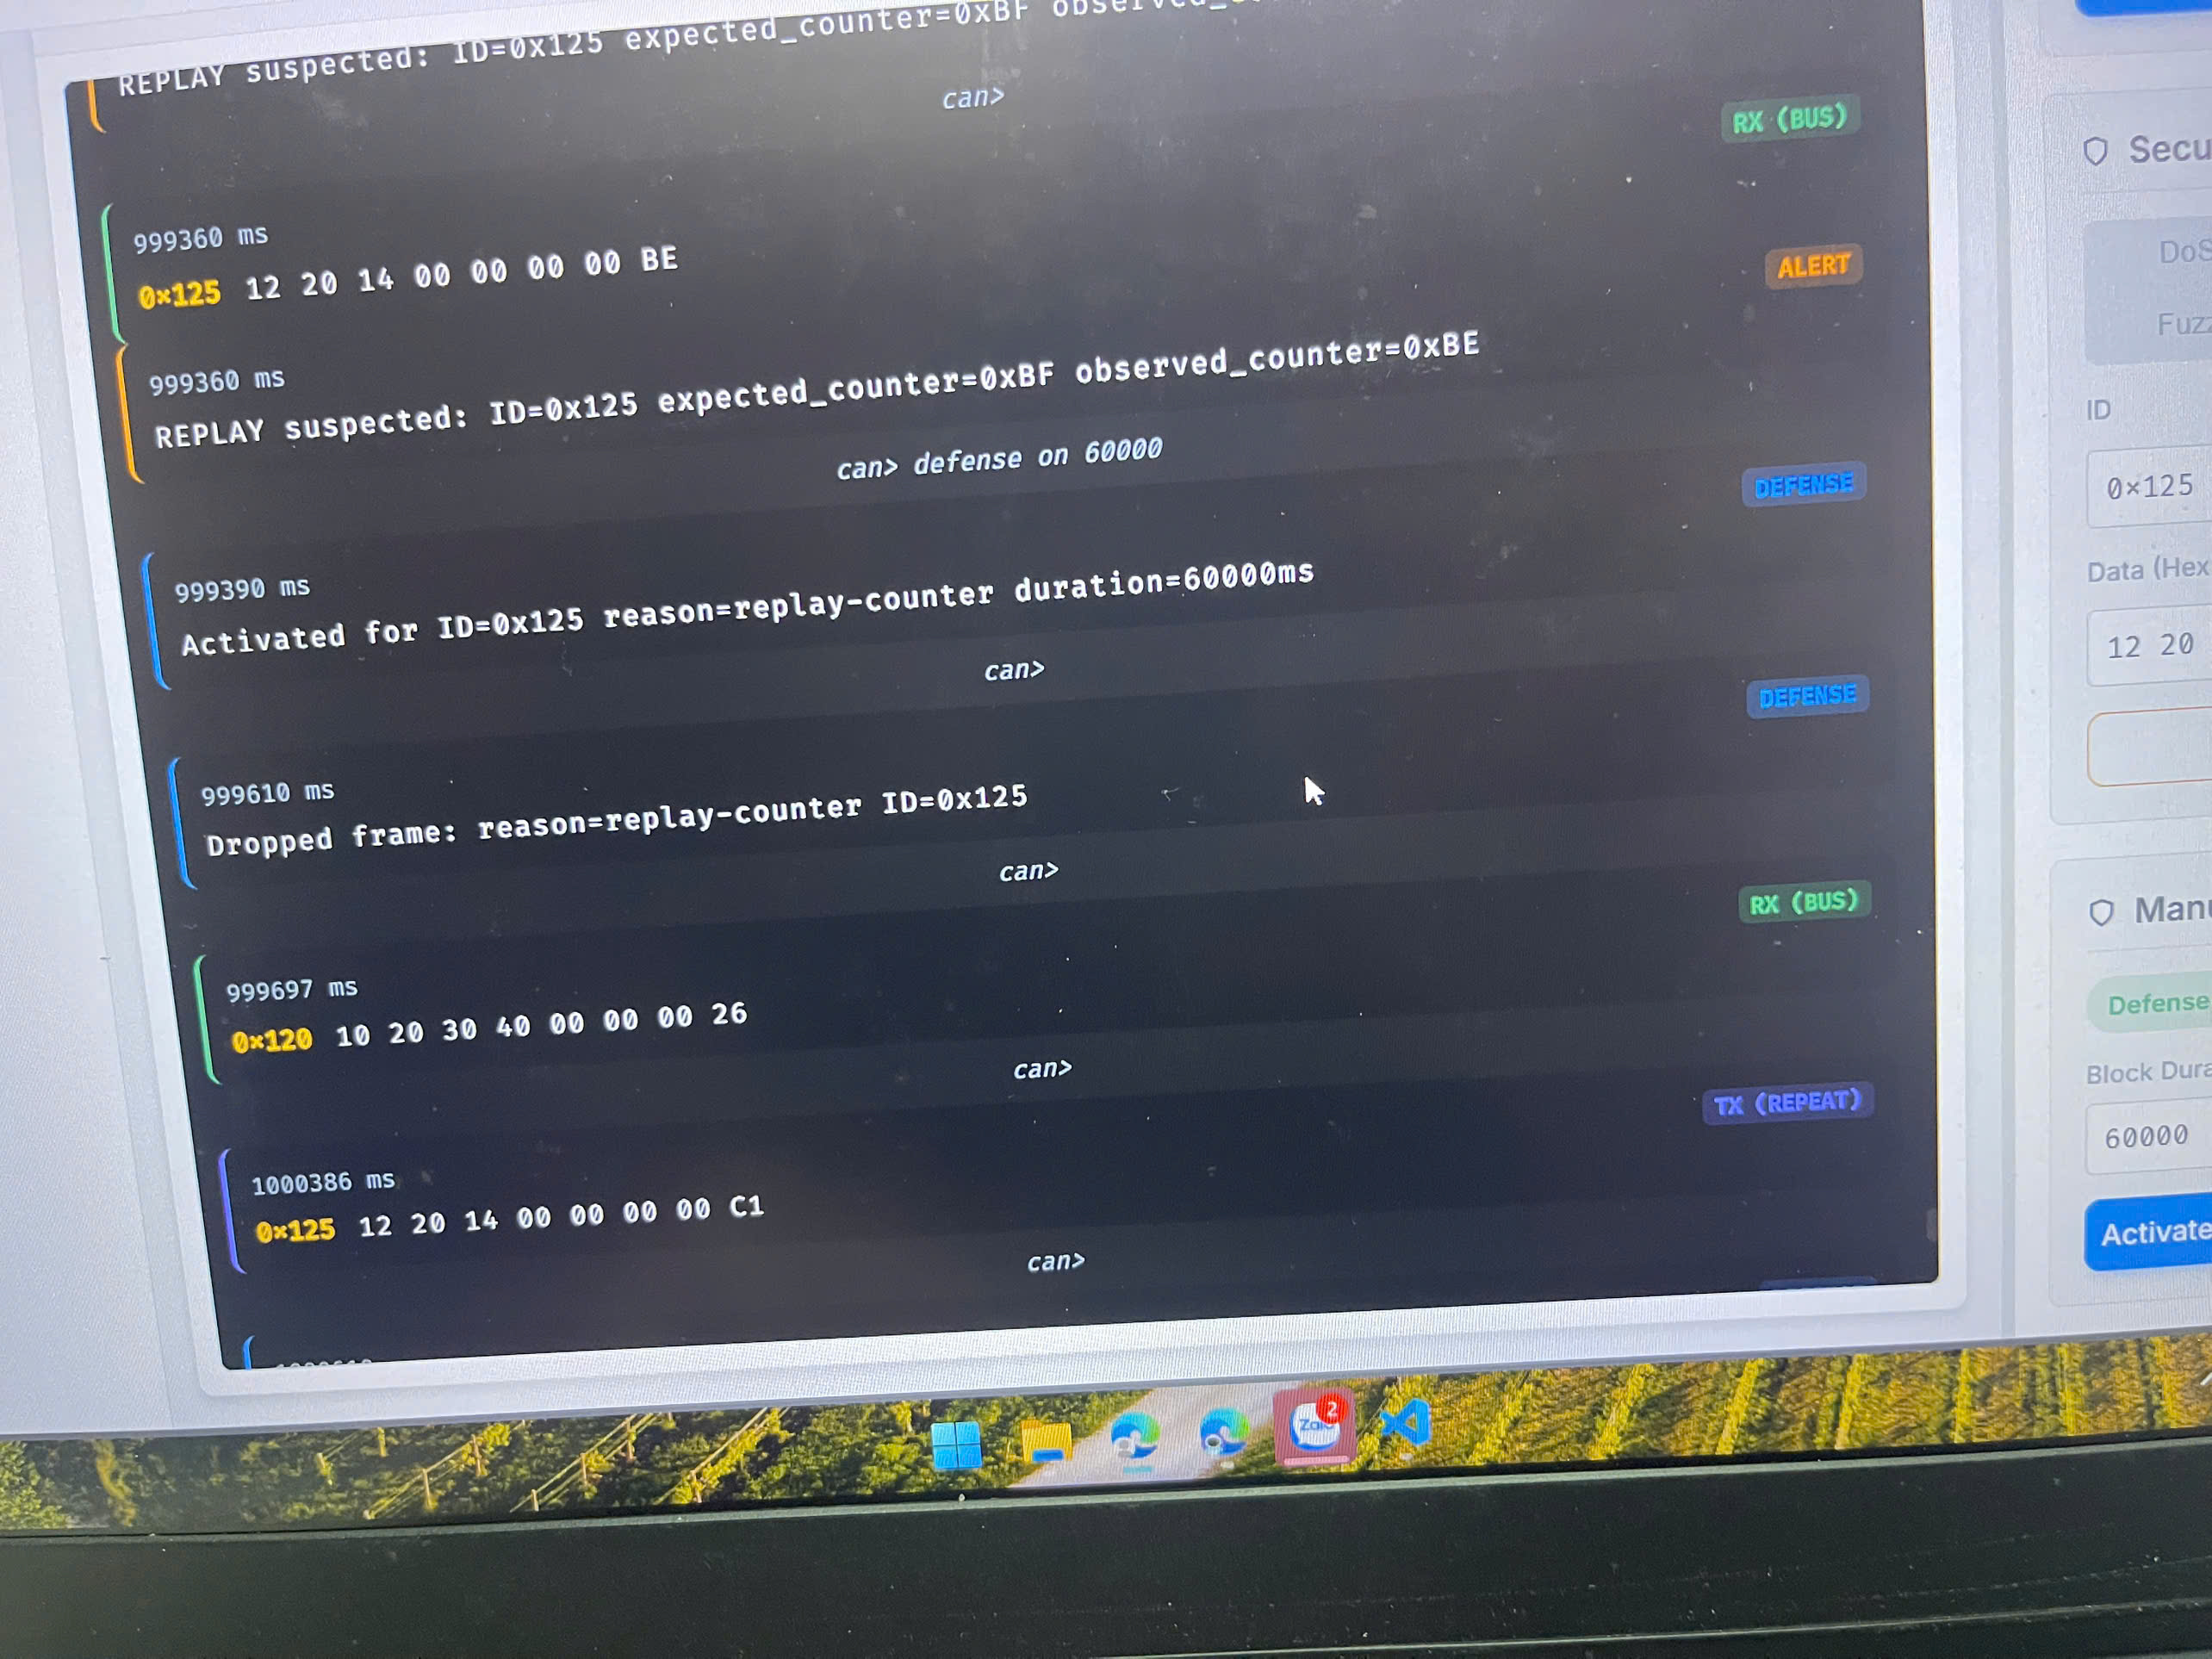
\includegraphics[width=0.75\textwidth]{images/replay_defend.png}
  \caption{Giao diện sau khi bật defense để chặn khung replay}
  \label{fig:replay-defend}
\end{figure}
}{%
\placeholderfigure{Ảnh log hiển thị trạng thái defense và các khung replay bị chặn}{Phòng thủ đối
với kịch bản Replay}
}

{\hbadness=10000
\textbf{Bước cảnh báo:} Ở Hình \ref{fig:replay-alert}, hệ thống tại nút nhận liên tục quan sát
thấy các khung mang ID \texttt{0x125} có giá trị bộ đếm cũ bị lặp lại. Hệ thống tiến hành so sánh
bộ đếm quan sát được với bộ đếm kỳ vọng và sinh ra cảnh báo \texttt{REPLAY suspected}, ví dụ
\texttt{expected\_counter=0xD2} \texttt{observed\_counter=0xBE}. Điều này minh chứng rằng cùng một
khung đã bị phát lại thay vì tiếp tục tăng tuần tự như trong phiên truyền hợp lệ.\par}

\textbf{Bước phòng thủ:} Ở Hình \ref{fig:replay-defend}, sau khi người vận hành gửi lệnh
\texttt{defense on 60000}, hệ thống xác nhận kích hoạt phòng thủ bằng thông báo
\texttt{Activated for ID=0x125 reason=replay-counter duration=60000ms}. Ngay sau đó, các
khung replay tiếp theo không còn được xử lý như dữ liệu hợp lệ mà bị ghi nhận dưới dạng
\texttt{Dropped frame: reason=replay-counter ID=0x125}. Cơ chế này giúp chặn luồng phát lại ở
tầng ứng dụng trong khi việc giám sát bus vẫn tiếp tục diễn ra.

\reportsubsection{3. Tấn công Fuzzing}

Trong kịch bản Fuzzing, nút tấn công liên tục thay đổi ID và dữ liệu tải để tạo ra chuỗi bản tin
bất thường, khó dự đoán. Mục tiêu của phần này là đánh giá khả năng phát hiện sự thay đổi
nhanh về mẫu lưu lượng, đặc biệt khi số lượng ID khác nhau tăng lên trong thời gian ngắn.

\IfFileExists{images/fuzzing_alert.png}{%
\begin{figure}[H]
  \centering
  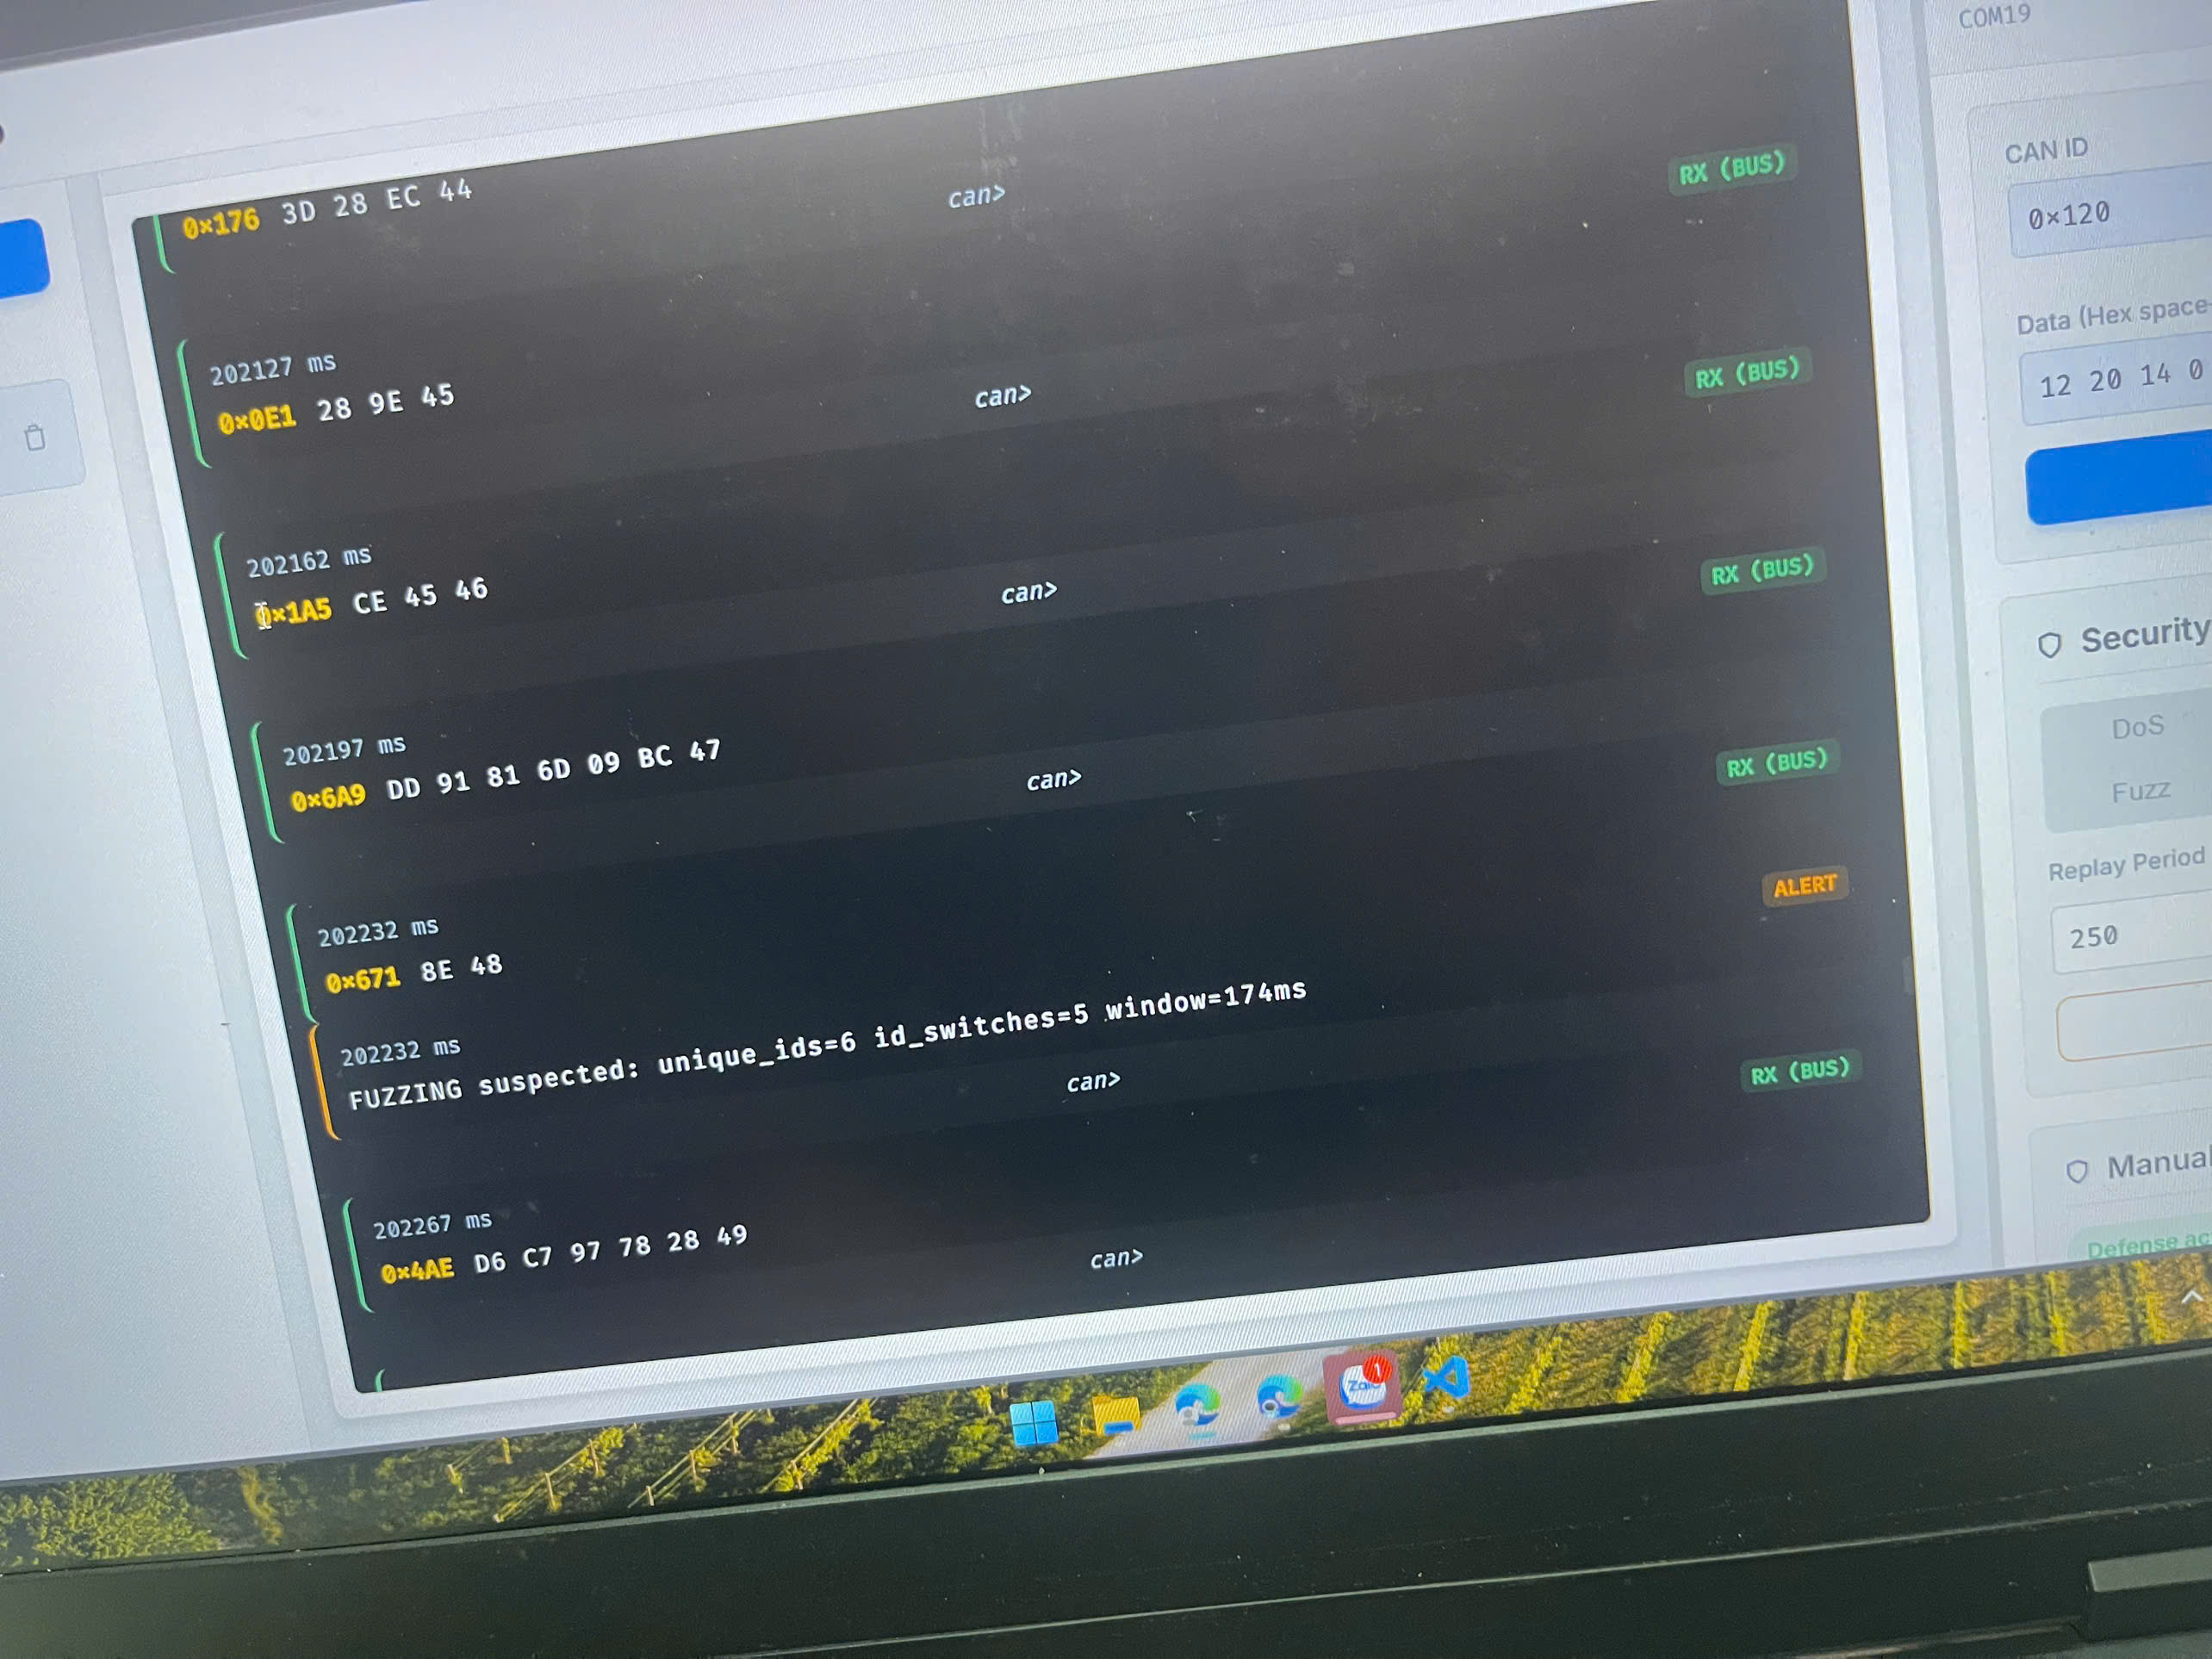
\includegraphics[width=0.98\textwidth]{images/fuzzing_alert.png}
  \caption{Giao diện ghi nhận cảnh báo ở giai đoạn phát hiện tấn công Fuzzing}
  \label{fig:fuzzing-alert}
\end{figure}
}{%
\placeholderfigure{Ảnh giao diện web khi xuất hiện cảnh báo fuzzing trên nút nhận}{Cảnh báo tấn
công Fuzzing}
}

Khi quan sát ở nút nhận, các bản tin xuất hiện với ID thay đổi nhanh và nội dung dữ liệu không
ổn định như trong chế độ truyền bình thường. Trong log, hệ thống có thể sinh cảnh báo
\texttt{FUZZING suspected} khi số lượng ID khác nhau và tần suất chuyển đổi ID vượt mức
cho phép.

\IfFileExists{images/fuzzing_defend.png}{%
\begin{figure}[H]
  \centering
  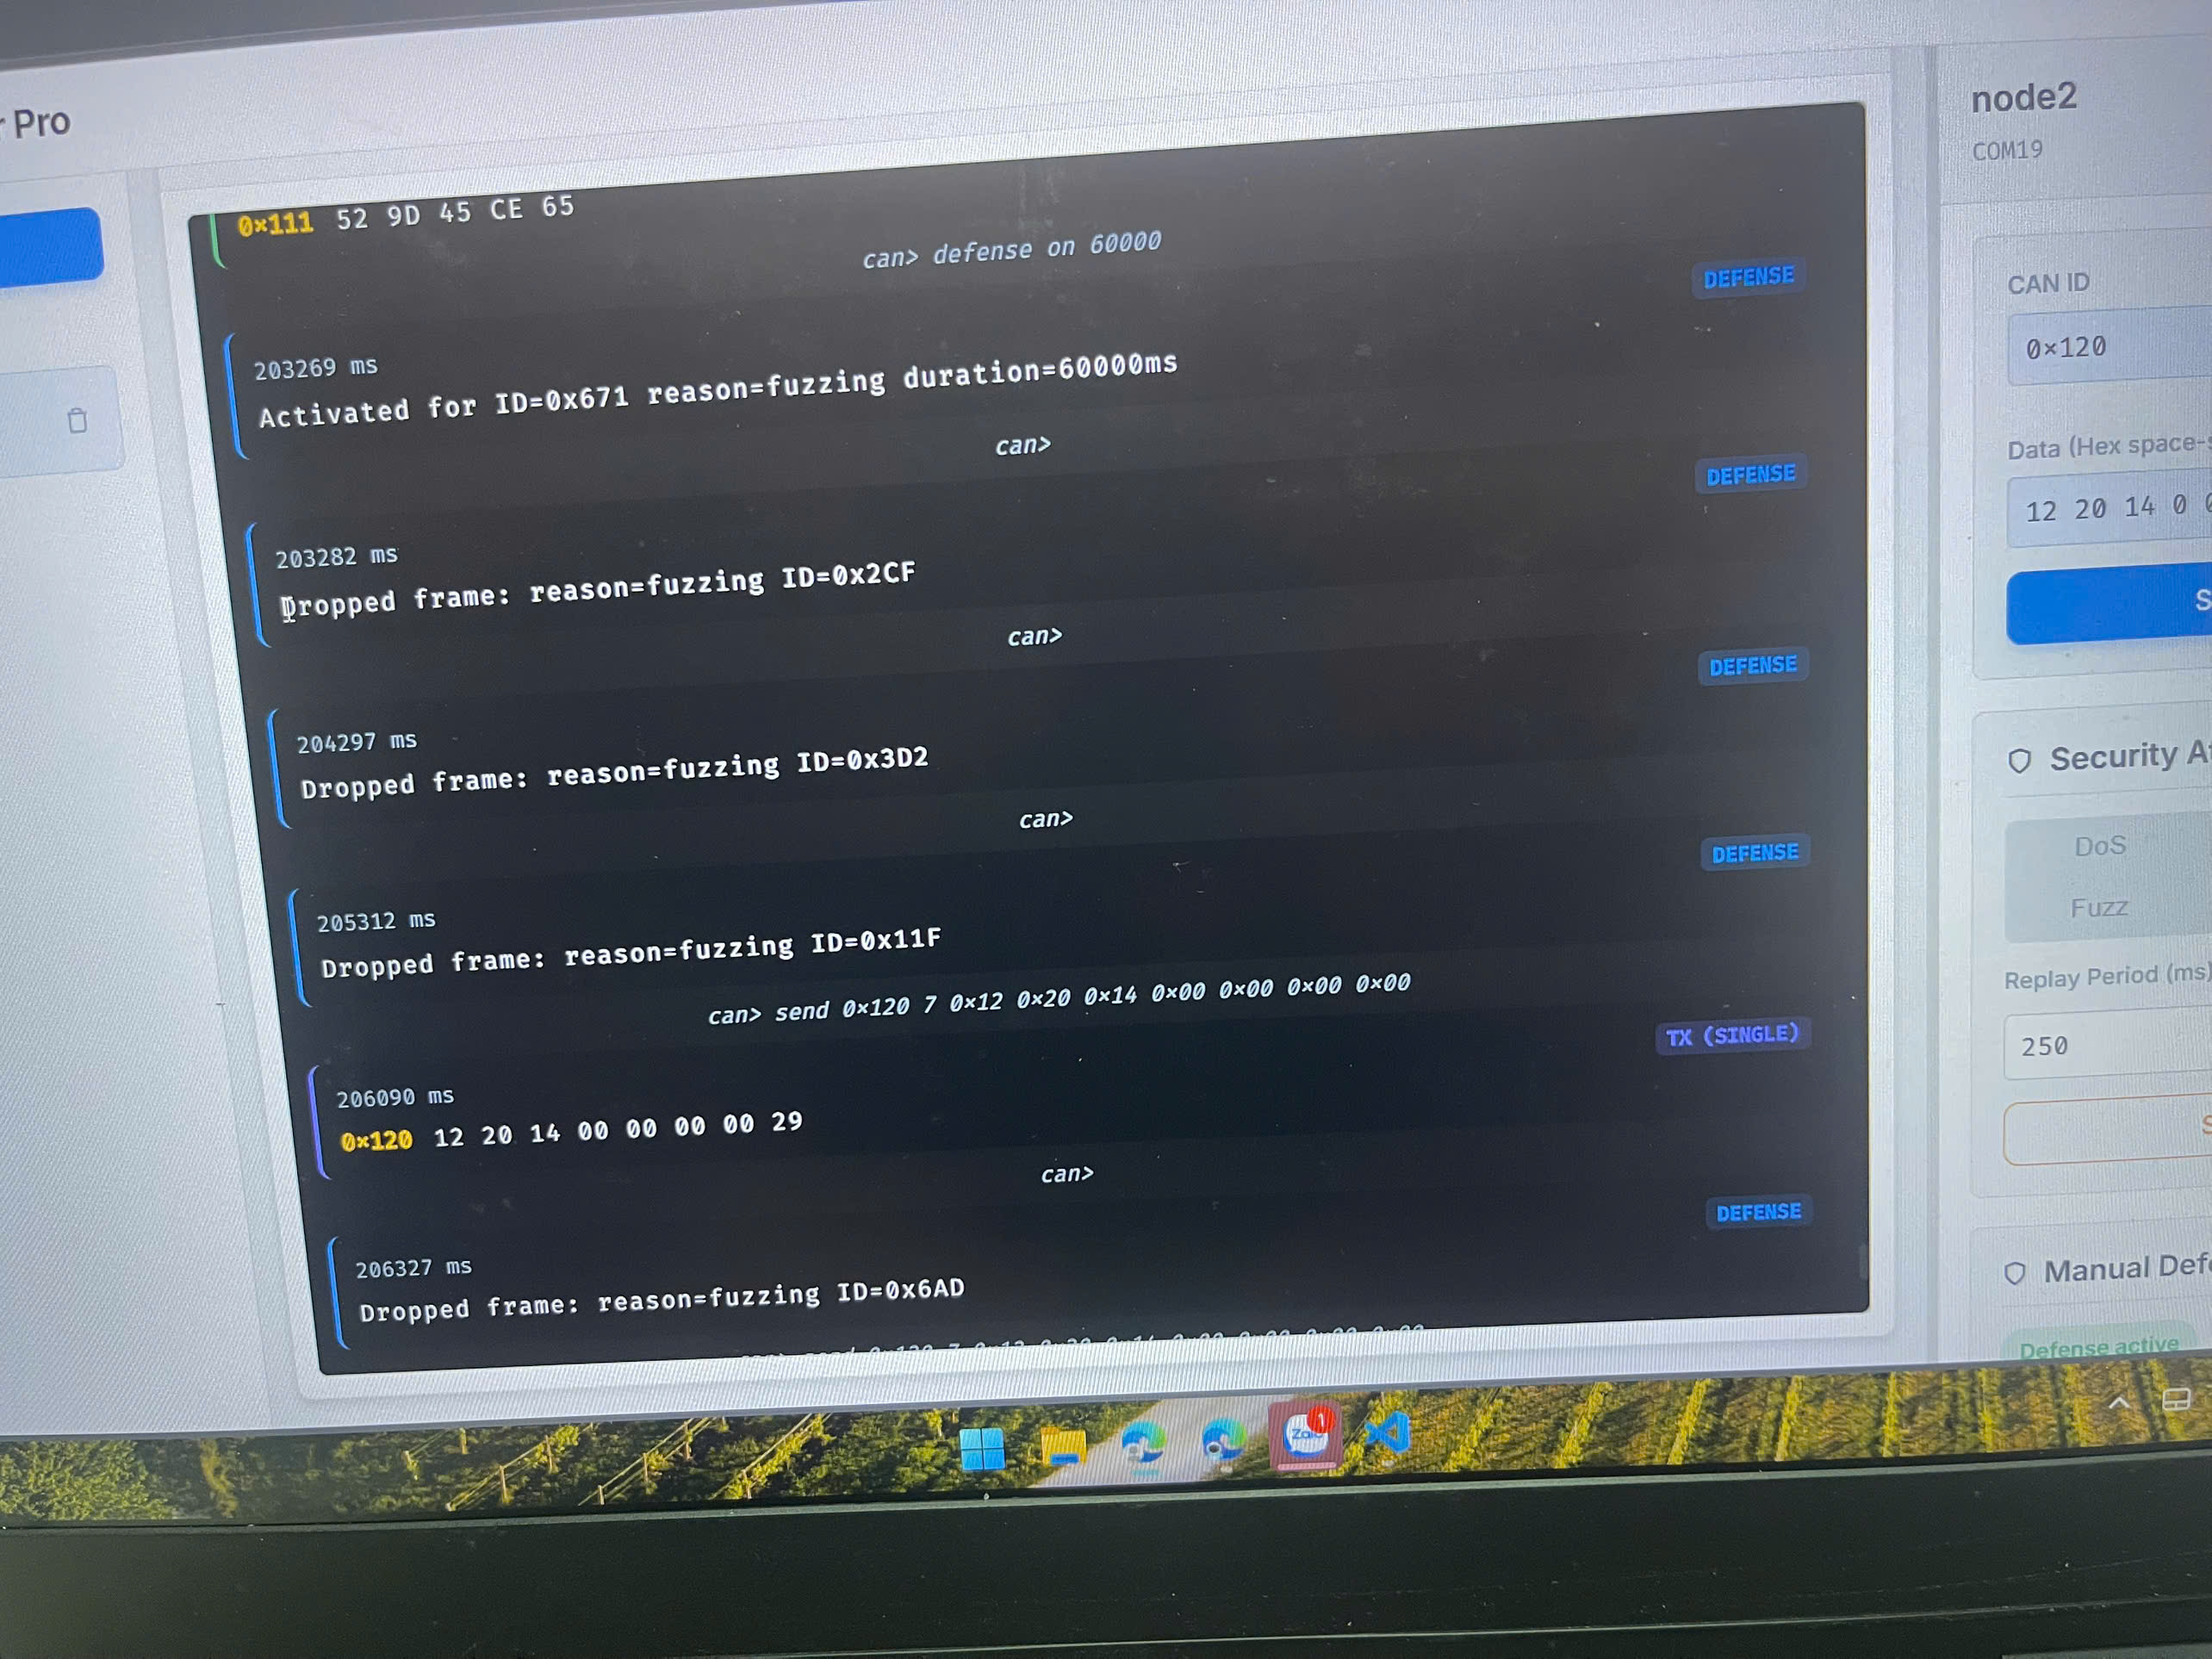
\includegraphics[width=0.98\textwidth]{images/fuzzing_defend.png}
  \caption{Giao diện sau khi bật defense để chặn lưu lượng Fuzzing}
  \label{fig:fuzzing-defend}
\end{figure}
}{%
\placeholderfigure{Ảnh log hiển thị trạng thái defense và các khung fuzzing bị chặn}{Phòng thủ đối
với kịch bản Fuzzing}
}

\textbf{Bước cảnh báo:} Ở Hình \ref{fig:fuzzing-alert}, nút nhận quan sát liên tiếp nhiều khung với
CAN ID thay đổi nhanh như \texttt{0x176}, \texttt{0x0E1}, \texttt{0x1A5}, \texttt{0x6A9},
\texttt{0x671}. Khi số lượng ID khác nhau và số lần chuyển đổi ID vượt ngưỡng, hệ thống sinh
cảnh báo \texttt{FUZZING suspected: unique\_ids=6 id\_switches=5 window=174ms}. Điều này
cho thấy lưu lượng đang bị tiêm nhiễu với mẫu phát không còn ổn định như giao tiếp bình
thường.

{\hbadness=10000
\textbf{Bước phòng thủ:} Ở Hình \ref{fig:fuzzing-defend}, ngay sau khi người vận hành tiến hành
gửi lệnh \texttt{defense on 60000}, hệ thống lập tức xác nhận kích hoạt thông qua thông báo
\texttt{Activated for ID=0x671} \texttt{reason=fuzzing} \texttt{duration=60000ms}. Sau đó, nhiều khung
lạ tiếp tục xuất hiện trên bus nhưng đã bị chặn ngay ở tầng ứng dụng với các dòng ghi log
\texttt{Dropped frame:} \texttt{reason=fuzzing} \texttt{ID=...}. Kết quả này chứng minh cơ chế phòng thủ
đã cô lập thành công luồng fuzzing mà vẫn cho phép các bản tin hợp lệ tiếp tục được quan sát.\par}

\reportsubsection{4. Tấn công Spoofing}

Trong kịch bản Spoofing, nút tấn công phát khung với cùng CAN ID của một thông điệp hợp lệ
nhưng thay đổi phần dữ liệu tải để giả mạo nội dung. Trước khi bắt đầu phần này, nên cho nút
hợp lệ gửi vài lần cùng một ID để hệ thống phía nhận có cơ sở xây dựng mẫu dữ liệu nền.

\IfFileExists{images/spoof_alert.png}{%
\begin{figure}[H]
  \centering
  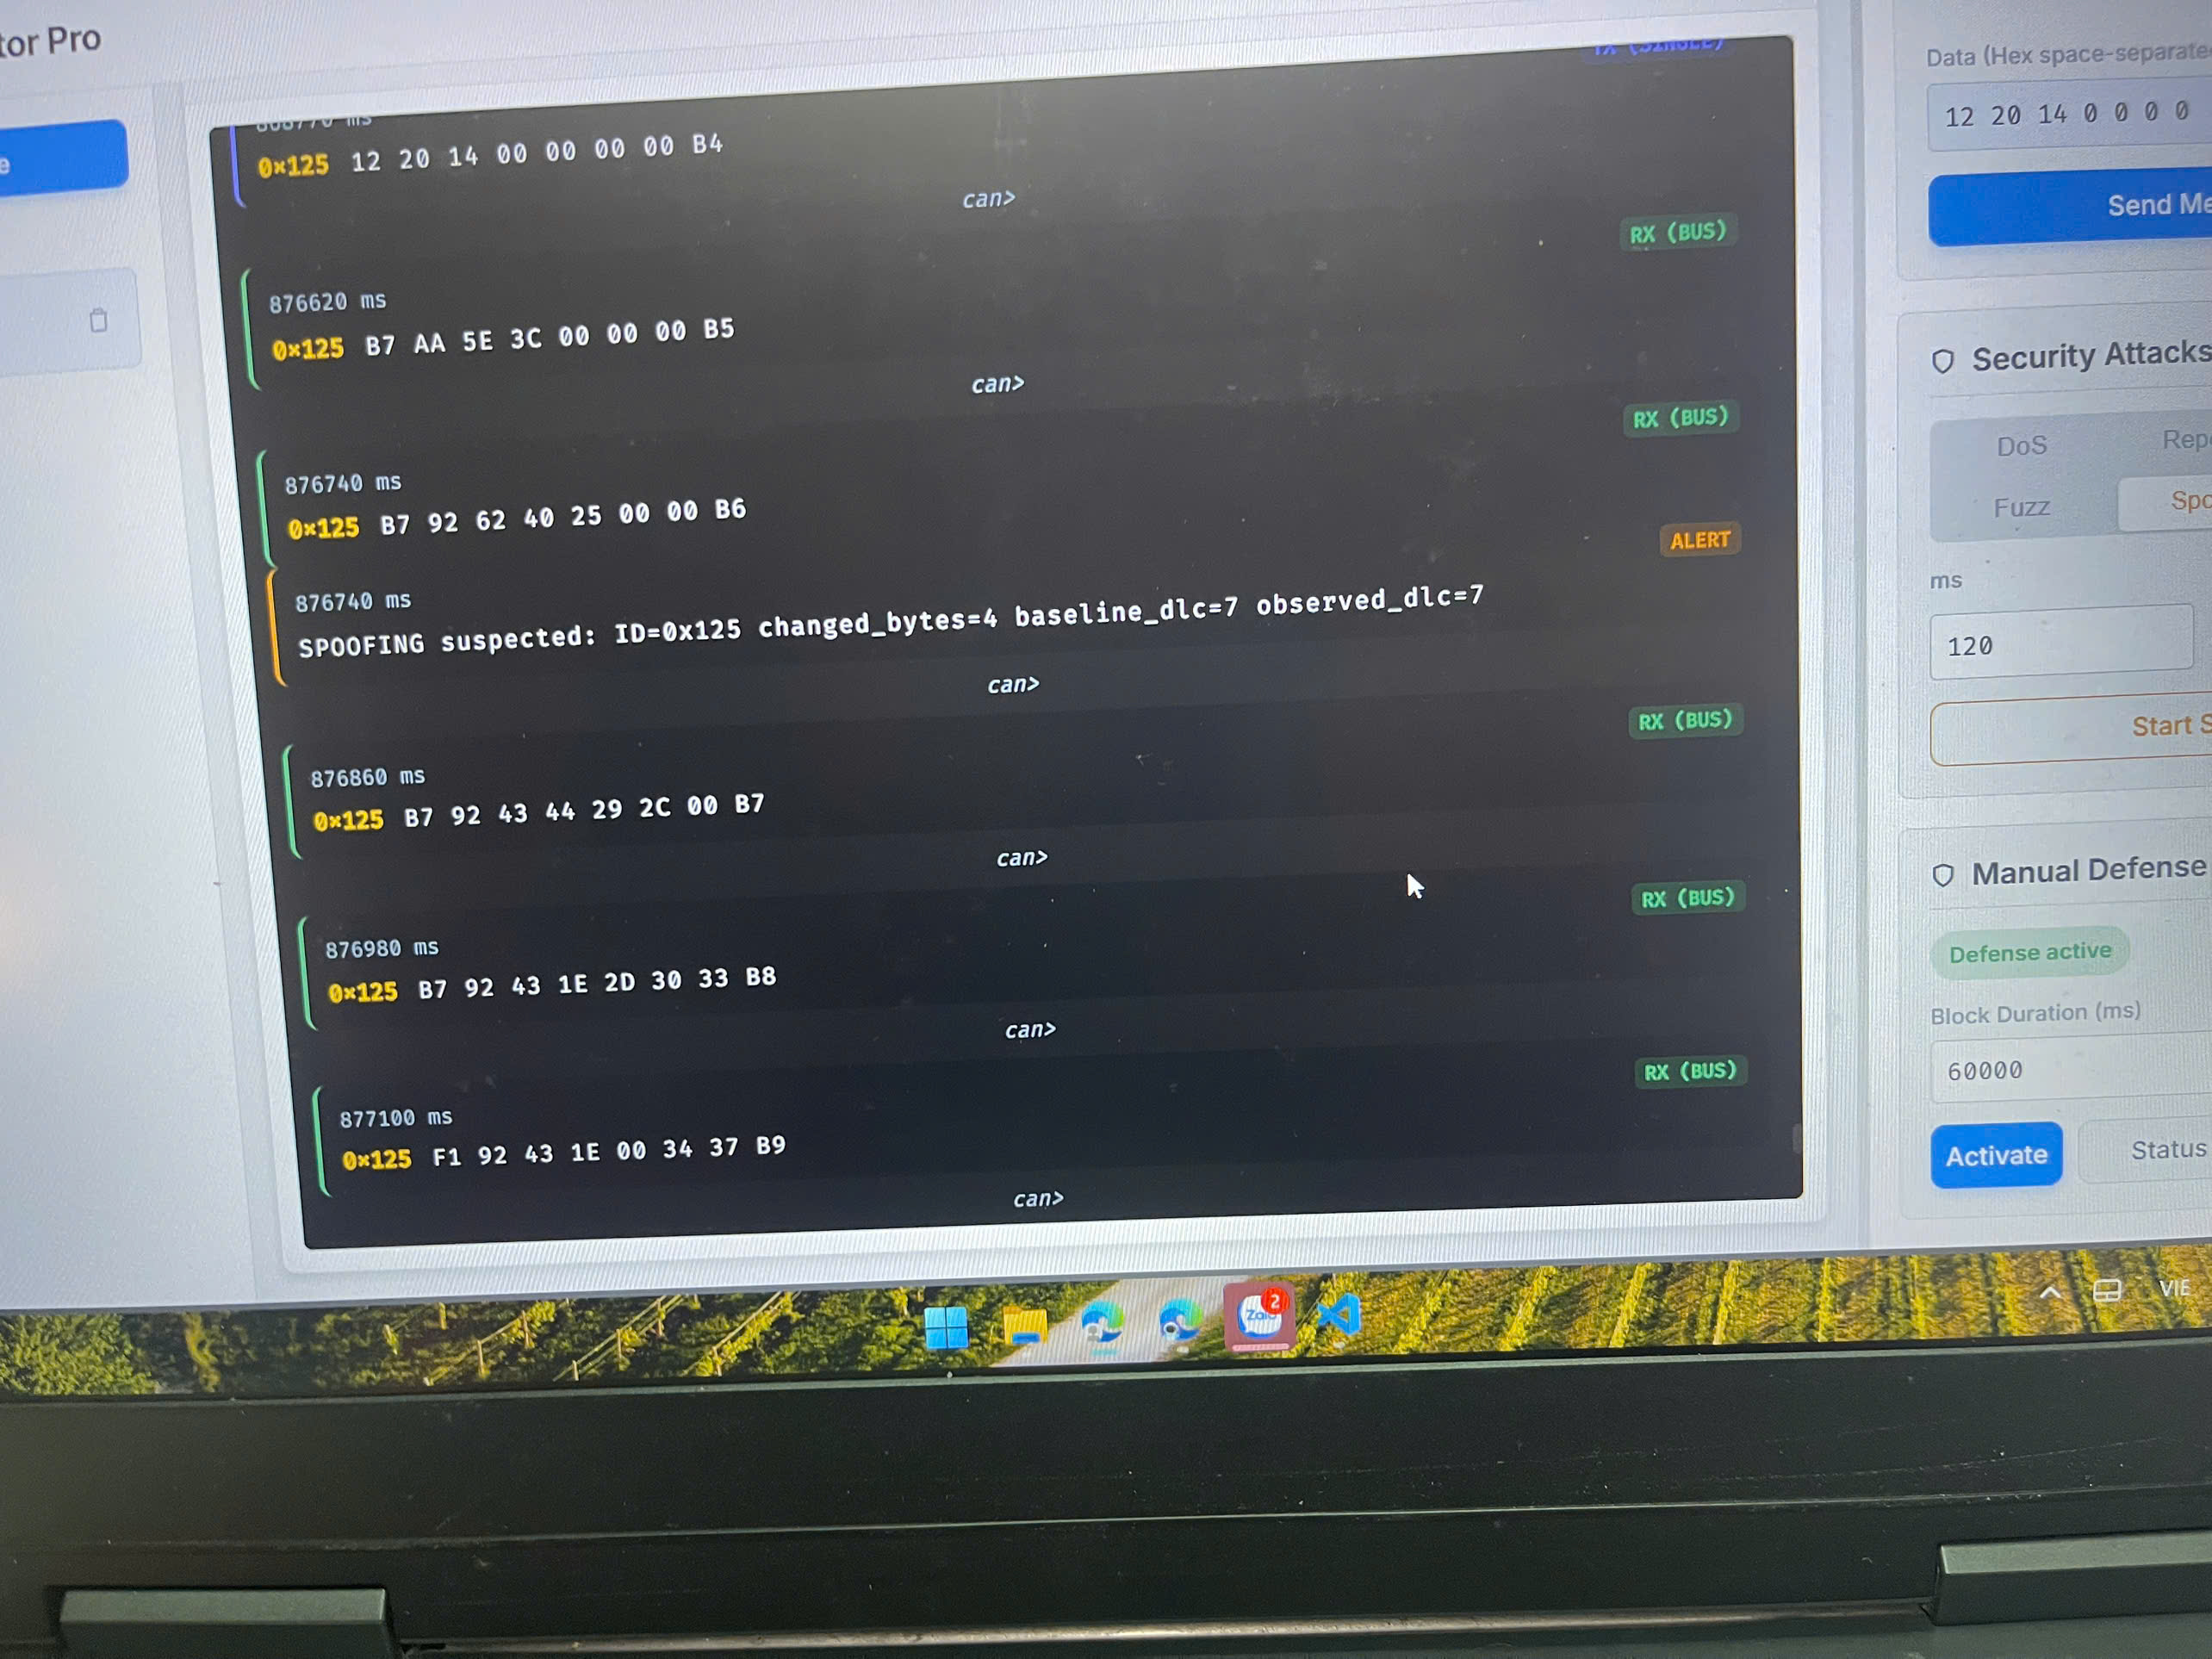
\includegraphics[width=0.98\textwidth]{images/spoof_alert.png}
  \caption{Giao diện ghi nhận cảnh báo ở giai đoạn phát hiện tấn công Spoofing}
  \label{fig:spoof-alert}
\end{figure}
}{%
\placeholderfigure{Ảnh giao diện khi xuất hiện cảnh báo spoofing trên nút nhận}{Cảnh báo tấn
công Spoofing}
}

Khi spoofing diễn ra, phía nhận vẫn thấy cùng một CAN ID quen thuộc nhưng phần dữ liệu thay
đổi bất thường so với mẫu hợp lệ trước đó. Đây là cơ sở để hệ thống sinh cảnh báo
\texttt{SPOOFING suspected} và phân biệt khung giả mạo với khung hợp lệ có cùng ID.

\IfFileExists{images/spoof_defend.png}{%
\begin{figure}[H]
  \centering
  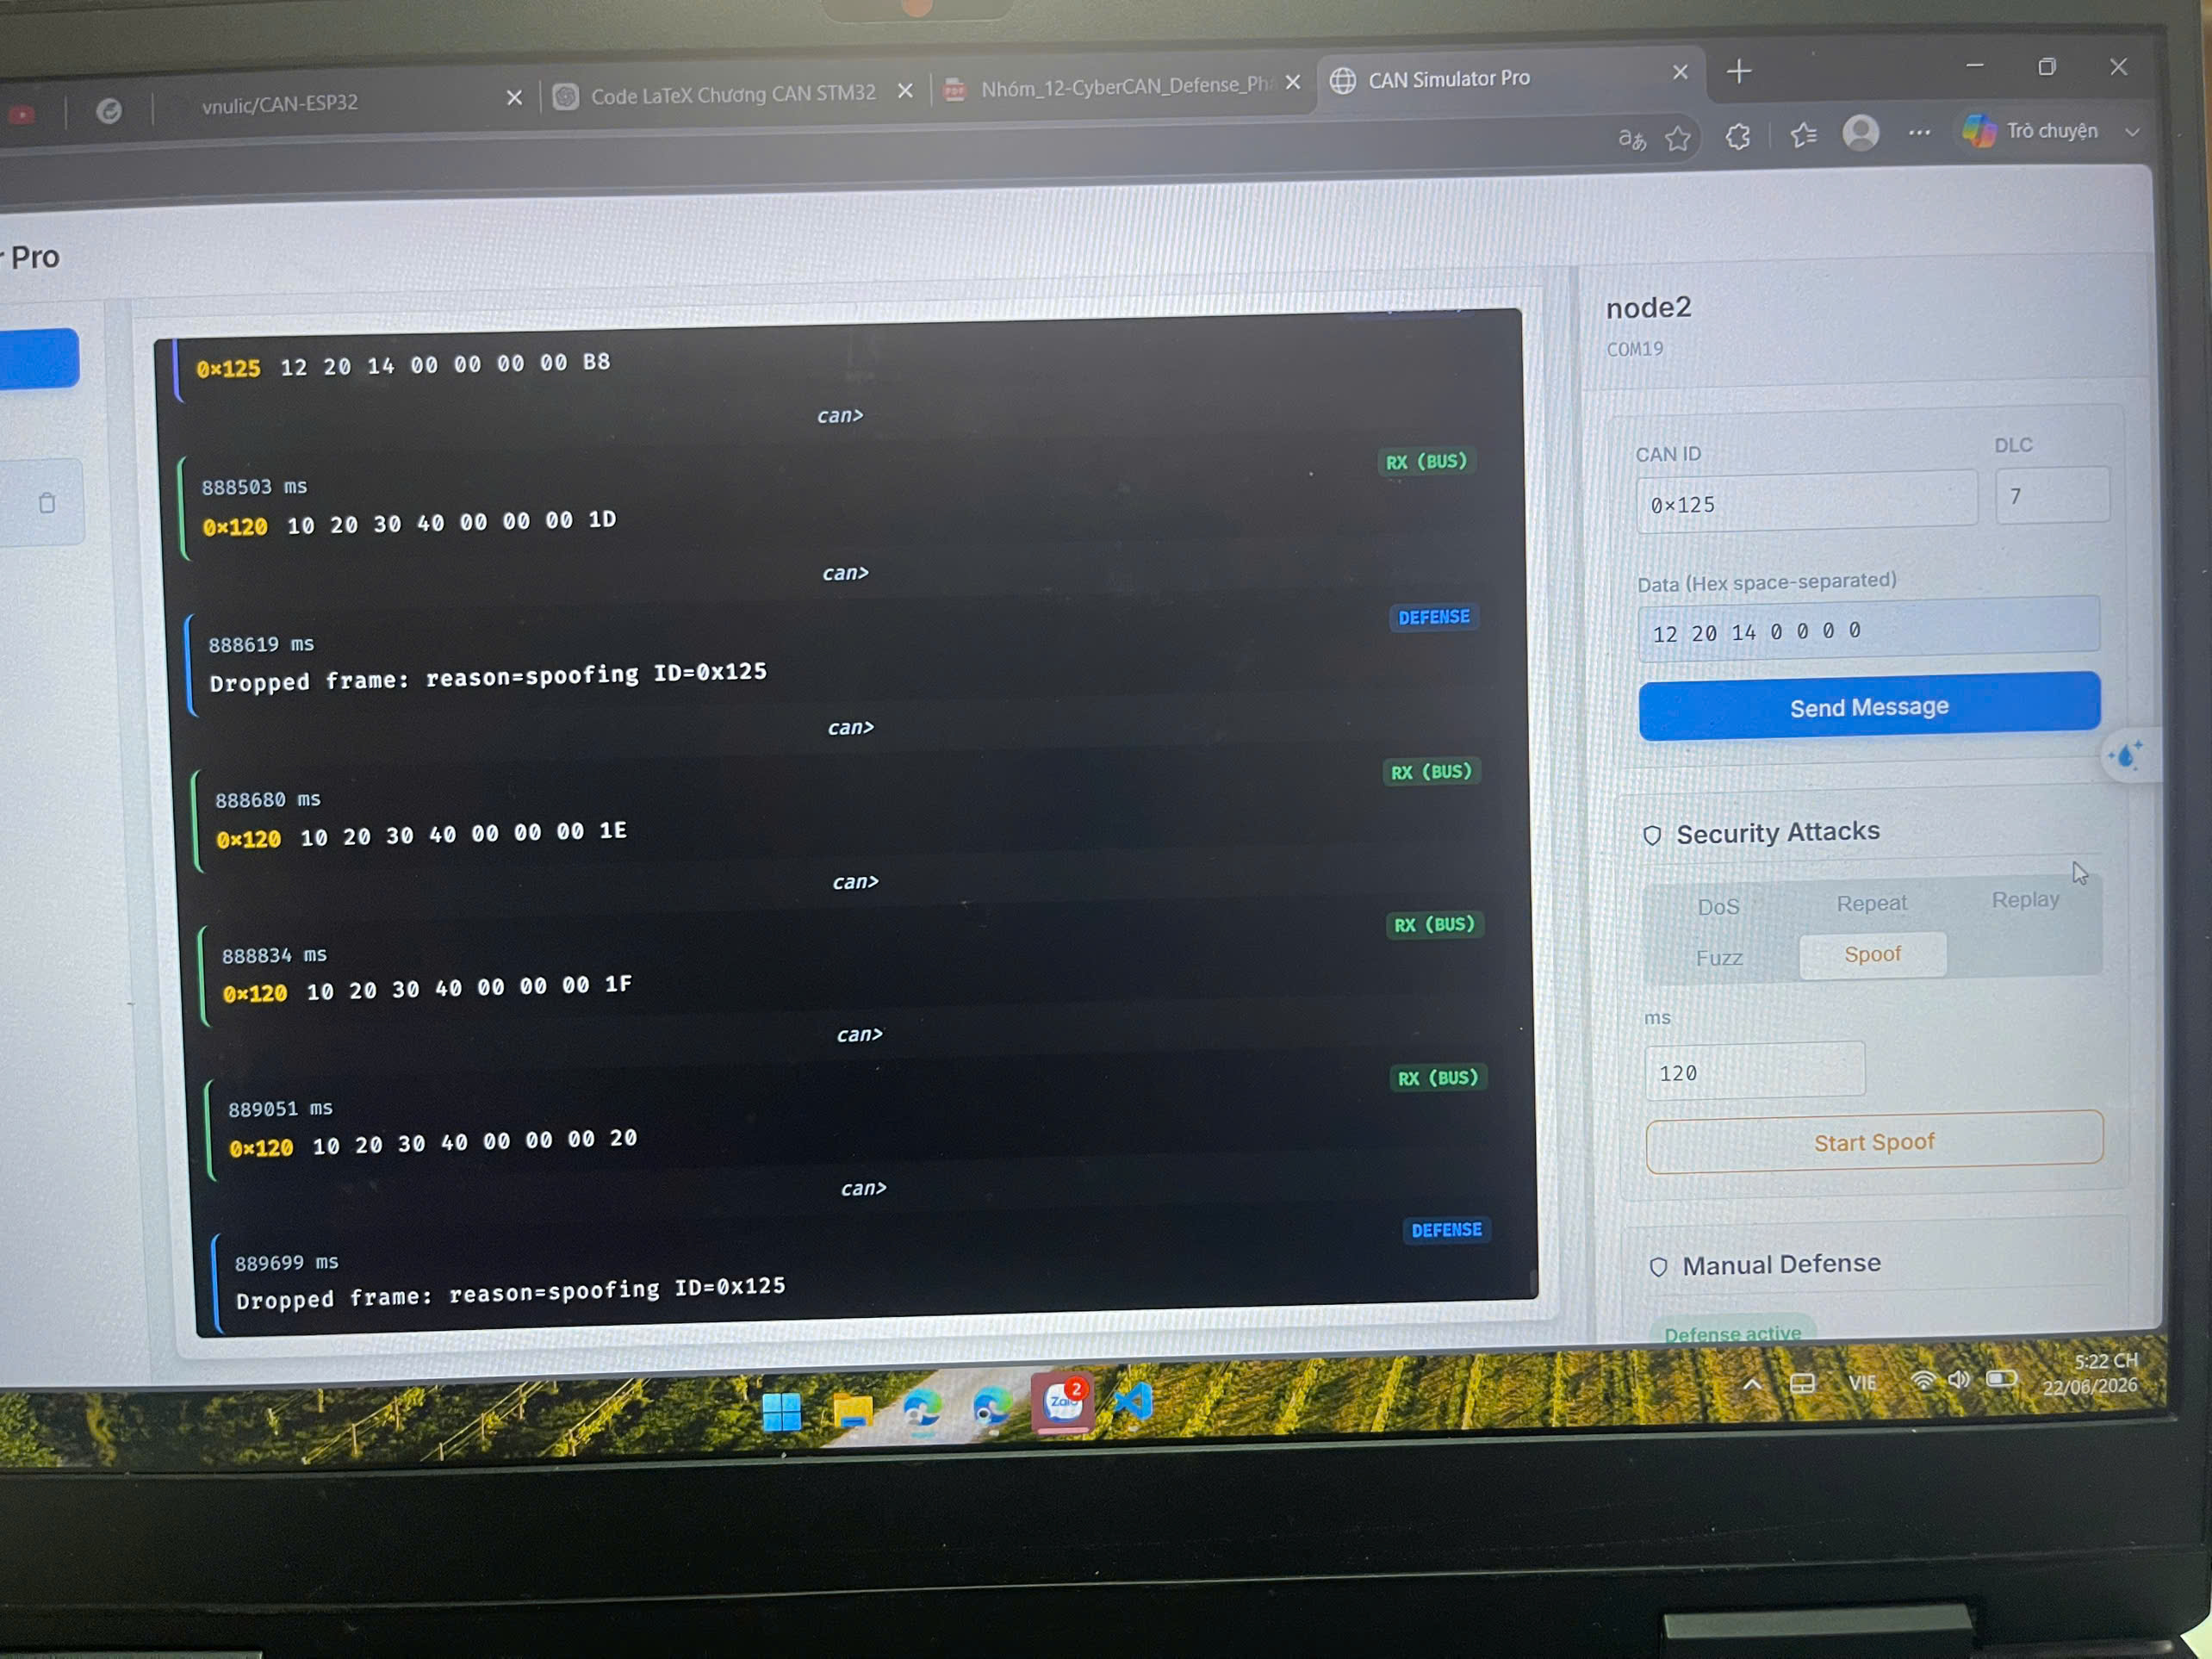
\includegraphics[width=0.98\textwidth]{images/spoof_defend.png}
  \caption{Giao diện sau khi bật defense để chặn khung spoofing}
  \label{fig:spoof-defend}
\end{figure}
}{%
\placeholderfigure{Ảnh log hiển thị trạng thái defense và các khung spoofing bị chặn}{Phòng thủ
đối với kịch bản Spoofing}
}

\textbf{Bước cảnh báo:} Ở Hình \ref{fig:spoof-alert}, nút nhận vẫn quan sát cùng CAN ID
\texttt{0x125} nhưng nội dung payload đã thay đổi rõ rệt so với mẫu hợp lệ trước đó. Từ sự sai
khác này, hệ thống sinh cảnh báo \texttt{SPOOFING suspected:} \texttt{ID=0x125} \texttt{changed\_bytes=4}
\texttt{baseline\_dlc=7} \texttt{observed\_dlc=7}. Đây là dấu hiệu cho thấy một khung giả mạo đang cố chèn
vào luồng giao tiếp bình thường.

\textbf{Bước phòng thủ:} Ở Hình \ref{fig:spoof-defend}, sau khi defense đã được bật, các khung
giả mạo cùng ID \texttt{0x125} không còn được xử lý như dữ liệu hợp lệ mà bị ghi nhận bằng
các dòng \texttt{Dropped frame: reason=spoofing ID=0x125}. Trong khi đó, các khung hợp lệ
khác như \texttt{0x120} vẫn tiếp tục xuất hiện trên giao diện. Điều này cho thấy cơ chế defense
đã chặn được luồng giả mạo theo đúng CAN ID nghi ngờ mà không làm gián đoạn hoàn toàn
quá trình giám sát bus.

Toàn bộ video minh họa cho các bước tấn công và phòng thủ của bốn kịch bản.

\begin{itemize}[leftmargin=*]
  \item \href{https://drive.google.com/drive/folders/1Ofl2Voi7a0QwBnF00v7ZM63E-JsUBCxc?usp=sharing}{\textcolor{blue}{Video tấn công và phòng thủ cho các kịch bản DoS, Replay, Fuzzing, Spoofing}}
\end{itemize}


\chapter{Tổng kết và hướng phát triển}

\section{Tổng kết}
Bài tập lớn ``CyberCAN Defense - Phát hiện và phòng thủ xâm nhập mạng nội bộ ô tô'' tập trung nghiên cứu giao thức CAN, phân tích các điểm yếu bảo mật đặc trưng của bus này và xây dựng một mô hình giám sát, phát hiện, phòng thủ trên nền tảng ESP32 \cite{bosch-can20,koscher2010,miller2015}.

Trong quá trình thực hiện, nhóm đã đạt được các kết quả nổi bật sau:
\begin{itemize}[leftmargin=*]
    \item \textbf{Nghiên cứu lý thuyết nền tảng:} Nhóm đã hệ thống lại các kiến thức quan trọng về CAN như cấu trúc khung dữ liệu, cơ chế phân xử ưu tiên, truyền thông broadcast, phát hiện lỗi và yêu cầu lớp vật lý của bus \cite{bosch-can20}.
    \item \textbf{Xây dựng mô hình hệ thống CAN thực tế:} Sử dụng các bo mạch vi điều khiển ESP32 và các module CAN của nhóm (dùng transceiver TJA1050 hoặc phần cứng tương đương), nhóm đã thiết lập mô hình bus CAN hai chiều giữa nhiều nút và máy tính giám sát \cite{espressif-twai,nxp-tja1050,bosch-can20}. Firmware được triển khai theo hướng gọn nhẹ, dễ kiểm thử và bám sát phần cứng thực tế của mô hình.
    \item \textbf{Thiết kế hệ thống truyền nhận cơ bản và có bảo vệ:}
    \begin{itemize}
        \item Luồng truyền nhận CAN cơ bản được xây dựng để mô phỏng hoạt động bình thường giữa các nút trong mạng \cite{koscher2010,miller2015}.
        \item Luồng có bảo vệ tích hợp bộ đếm thông điệp, phát hiện lặp khung, phát hiện ngập lưu lượng và cơ chế chặn theo CAN ID khi có cảnh báo \cite{koscher2010,miller2015}.
    \end{itemize}
    \item \textbf{Mô phỏng tấn công và phòng thủ:}
    \begin{itemize}
        \item Hệ thống hỗ trợ mô phỏng các kịch bản replay, spoofing theo chu kỳ và spam/DoS thông qua các lệnh điều khiển trên terminal \cite{koscher2010,miller2015}.
        \item Cơ chế phòng thủ cho phép phát hiện bản tin bất thường và cô lập tạm thời các CAN ID bị nghi ngờ ở mức ứng dụng \cite{koscher2010,miller2015}.
    \end{itemize}
    \item \textbf{Xây dựng giao diện trực quan bằng website:} Ứng dụng web dùng FastAPI, WebSocket và kết nối serial để theo dõi bản tin CAN, hiển thị cảnh báo, điều khiển tấn công và kích hoạt phòng thủ từ giao diện tập trung \cite{fastapi-docs,pyserial-docs}.
    \item \textbf{Minh họa kết quả qua thực nghiệm:} Mô hình phần cứng và phần mềm của đề tài cho thấy khả năng trình diễn rõ ràng luồng truyền CAN cơ bản, kịch bản tấn công và phản ứng của cơ chế bảo vệ trên cùng một hệ thống.
\end{itemize}

Kết quả của dự án cho thấy cách tiếp cận phát hiện bất thường kết hợp chặn theo ID có thể nâng cao khả năng quan sát và giảm tác động của các bản tin nghi ngờ trong mô hình CAN thử nghiệm \cite{koscher2010,miller2015}. Đây là nền tảng phù hợp để tiếp tục phát triển các cơ chế bảo mật mạnh hơn cho mạng truyền thông nội bộ ô tô.

\section{Ứng dụng Trí tuệ Nhân tạo (AI)}

Trong quá trình thực hiện dự án CyberCAN Defense: Phát hiện và Phòng thủ Xâm nhập Mạng Nội bộ Ô tô, nhóm đã sử dụng nhiều công cụ Trí tuệ Nhân tạo (AI) khác nhau nhằm hỗ trợ nghiên cứu, thiết kế hệ thống, phát triển phần mềm và xây dựng tài liệu kỹ thuật. Mỗi công cụ được sử dụng cho những mục đích khác nhau dựa trên thế mạnh riêng, bao gồm ChatGPT, Claude và Prism AI. Việc kết hợp các công cụ AI đã giúp nhóm rút ngắn thời gian nghiên cứu, nâng cao hiệu quả làm việc và hỗ trợ giải quyết nhiều vấn đề kỹ thuật trong quá trình thực hiện đề tài.

\subsection{Ứng dụng ChatGPT trong nghiên cứu và thiết kế hệ thống}

ChatGPT được sử dụng chủ yếu trong giai đoạn nghiên cứu lý thuyết, tìm hiểu công nghệ và hỗ trợ thiết kế hệ thống. Trong quá trình tìm hiểu kiến thức nền tảng, ChatGPT hỗ trợ giải thích các khái niệm liên quan đến giao thức CAN Bus, cấu trúc CAN Frame, cơ chế Arbitration, Error Detection, Error Handling, Bit Stuffing cũng như nguyên lý hoạt động của bộ điều khiển TWAI trên ESP32 và bộ chuyển đổi CAN TJA1050.

Bên cạnh đó, ChatGPT còn được sử dụng để tìm hiểu các nội dung chuyên sâu về an ninh mạng ô tô, bao gồm các hình thức tấn công phổ biến trên mạng CAN như Replay Attack, Spoofing Attack, Denial of Service (DoS), Fuzzing Attack, Message Injection Attack và các phương pháp phát hiện xâm nhập đang được sử dụng trong các hệ thống IDS hiện đại. Công cụ này giúp nhóm tiếp cận nhanh với các kiến thức mới, giải thích các thuật ngữ chuyên ngành và đề xuất các hướng nghiên cứu phù hợp với phạm vi của đề tài.

Trong giai đoạn thiết kế hệ thống, ChatGPT hỗ trợ xây dựng kiến trúc tổng thể của dự án, đề xuất các phương án kết nối giữa ESP32, TJA1050, CAN Bus, Node Attacker, Node Defender và giao diện Web Monitoring. Công cụ cũng hỗ trợ xây dựng sơ đồ khối hệ thống, sơ đồ luồng dữ liệu, lưu đồ thuật toán và các sơ đồ minh họa phục vụ cho quá trình thiết kế và trình bày báo cáo. Ngoài ra, ChatGPT còn hỗ trợ giải thích kiến trúc AUTOSAR, phân tích mối liên hệ giữa dự án CyberCAN Defense và các thành phần trong AUTOSAR Classic Platform, từ đó giúp nhóm xây dựng phần đánh giá và định hướng phát triển của hệ thống theo các tiêu chuẩn công nghiệp.

Trong quá trình xây dựng báo cáo, ChatGPT được sử dụng để hỗ trợ tổng hợp thông tin từ nhiều nguồn tài liệu, giải thích các khái niệm kỹ thuật, đề xuất nội dung cho các chương báo cáo và hỗ trợ chuẩn hóa cách diễn đạt theo phong cách học thuật.

\subsection{Ứng dụng Claude trong phát triển và kiểm thử phần mềm}

Claude được sử dụng chủ yếu trong quá trình phát triển phần mềm và xử lý các vấn đề liên quan đến mã nguồn. Công cụ hỗ trợ giải thích cách sử dụng các thư viện lập trình trên ESP32, đề xuất cấu trúc chương trình và hỗ trợ xây dựng các module chức năng như truyền nhận CAN Frame, Web Server, WebSocket, giao diện giám sát thời gian thực và các cơ chế phát hiện tấn công.

Trong quá trình lập trình, Claude được sử dụng để hỗ trợ phân tích lỗi biên dịch, lỗi logic và các vấn đề phát sinh trong quá trình truyền nhận dữ liệu CAN. Công cụ hỗ trợ giải thích nguyên nhân gây lỗi, đề xuất các phương pháp khắc phục và đưa ra các gợi ý tối ưu hóa mã nguồn nhằm nâng cao tính ổn định của hệ thống. Đối với các thuật toán phát hiện tấn công, Claude hỗ trợ phân tích tính hợp lý của các điều kiện phát hiện, đánh giá độ hiệu quả của từng phương pháp và đề xuất các cải tiến phù hợp với khả năng xử lý của ESP32.

Trong giai đoạn kiểm thử, Claude được sử dụng để hỗ trợ xây dựng các kịch bản mô phỏng tấn công, đề xuất các trường hợp thử nghiệm và hỗ trợ phân tích dữ liệu CAN thu thập được trong quá trình thực nghiệm. Công cụ cũng hỗ trợ kiểm tra tính nhất quán của mã nguồn, rà soát các lỗi tiềm ẩn và đánh giá hiệu quả hoạt động của hệ thống IDS trước các tình huống tấn công khác nhau.

Ngoài ra, Claude còn được sử dụng để hỗ trợ xây dựng và hiệu chỉnh mã nguồn cho các thành phần Web Monitoring, xử lý dữ liệu thời gian thực và các chức năng hỗ trợ người dùng trong quá trình quan sát trạng thái mạng CAN.

\subsection{Ứng dụng Prism AI trong xây dựng tài liệu và thuyết trình}

Prism AI được sử dụng chủ yếu trong quá trình xây dựng báo cáo và chuẩn hóa tài liệu kỹ thuật. Công cụ hỗ trợ kiểm tra chính tả, ngữ pháp và tính nhất quán của nội dung, đồng thời đề xuất các cách diễn đạt phù hợp với văn phong học thuật và kỹ thuật.

Trong quá trình biên soạn báo cáo bằng LaTeX, Prism AI hỗ trợ xây dựng cấu trúc chương mục, đề xuất cách tổ chức nội dung, định dạng bảng biểu, hình ảnh và các thành phần trình bày khác nhằm nâng cao tính trực quan của tài liệu. Công cụ cũng hỗ trợ rà soát lỗi định dạng, đề xuất các cải tiến về bố cục và đảm bảo tính thống nhất giữa các chương trong báo cáo.

Bên cạnh đó, Prism AI còn được sử dụng để hỗ trợ xây dựng nội dung thuyết trình, đề xuất bố cục slide, cách trình bày các sơ đồ kỹ thuật, biểu đồ và các nội dung minh họa nhằm giúp quá trình trình bày đề tài trở nên rõ ràng và dễ tiếp cận hơn.

\subsection{Đánh giá hiệu quả sử dụng AI trong dự án}

Việc kết hợp ChatGPT, Claude và Prism AI trong các giai đoạn khác nhau của dự án đã giúp nhóm nâng cao hiệu quả nghiên cứu, đẩy nhanh tiến độ phát triển hệ thống và cải thiện chất lượng tài liệu kỹ thuật. ChatGPT hỗ trợ mạnh trong việc nghiên cứu lý thuyết, thiết kế kiến trúc và xây dựng sơ đồ; Claude hỗ trợ hiệu quả trong phát triển phần mềm, phân tích lỗi và kiểm thử hệ thống; trong khi Prism AI hỗ trợ chuẩn hóa báo cáo và nâng cao chất lượng trình bày tài liệu.

Tuy nhiên, các công cụ AI chỉ đóng vai trò hỗ trợ trong quá trình thực hiện đề tài. Mọi quyết định về lựa chọn kiến trúc hệ thống, triển khai phần cứng, phát triển phần mềm, xây dựng cơ chế phát hiện tấn công, thực hiện thí nghiệm và đánh giá kết quả cuối cùng đều do các thành viên trong nhóm trực tiếp thực hiện và chịu trách nhiệm.
\section{Liên hệ với kiến trúc phần mềm AUTOSAR}

\subsection{Tổng quan về AUTOSAR}

AUTOSAR (AUTomotive Open System ARchitecture) là tiêu chuẩn kiến trúc phần mềm được phát triển dành cho các hệ thống điện tử trên ô tô hiện đại. Mục tiêu của AUTOSAR là chuẩn hóa cách xây dựng phần mềm trên các ECU (Electronic Control Unit), cho phép các thành phần phần mềm được tái sử dụng trên nhiều nền tảng phần cứng khác nhau, đồng thời giảm chi phí phát triển và tăng khả năng tương thích giữa các nhà sản xuất.

Trong AUTOSAR Classic Platform, hệ thống được tổ chức theo kiến trúc phân lớp bao gồm Application Layer, Runtime Environment (RTE) và Basic Software (BSW). Application Layer chứa các chức năng điều khiển của xe như động cơ, phanh ABS, túi khí hoặc các chức năng an ninh mạng. Runtime Environment đóng vai trò trung gian cho phép các thành phần phần mềm giao tiếp với nhau mà không phụ thuộc trực tiếp vào phần cứng. Basic Software cung cấp các dịch vụ nền tảng như hệ điều hành, giao tiếp CAN, quản lý bộ nhớ, chẩn đoán lỗi và các trình điều khiển thiết bị.

\begin{figure}[H]
	\centering
	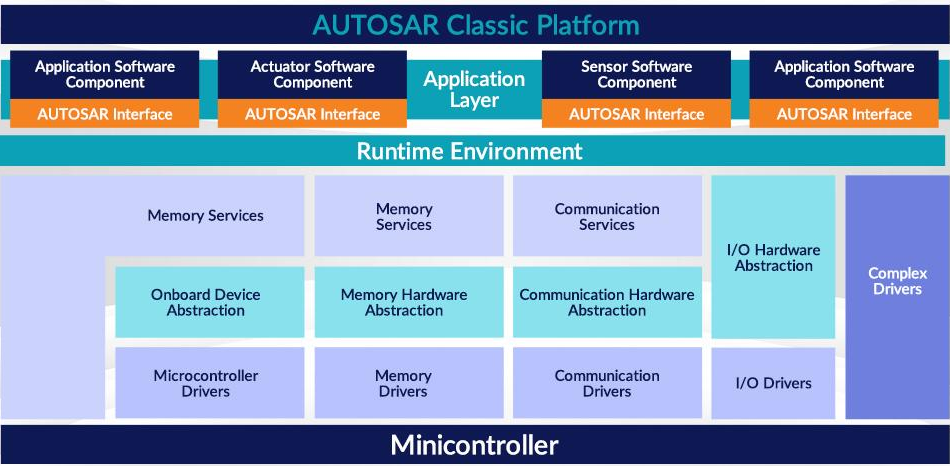
\includegraphics[width=0.75\textwidth]{images/AUTOSAR.png}
	\caption{AUTOSAR Classic Platform Architecture}
\end{figure}

Kiến trúc phân lớp này giúp tách biệt phần mềm ứng dụng khỏi phần cứng, tạo điều kiện cho việc bảo trì, nâng cấp và phát triển các chức năng mới trên xe một cách hiệu quả hơn. Hiện nay, AUTOSAR Classic được sử dụng rộng rãi trong các ECU điều khiển động cơ, hệ thống phanh, hệ thống thân xe và các hệ thống điều khiển thời gian thực trên ô tô.

\subsection{Khả năng tích hợp AUTOSAR với dự án}

Trong hệ thống, ESP32 đóng vai trò tương tự bộ vi điều khiển trung tâm của một ECU. Bộ chuyển đổi CAN TJA1050 thực hiện chức năng tương đương tầng CAN Transceiver, chịu trách nhiệm chuyển đổi tín hiệu logic từ bộ điều khiển CAN thành tín hiệu vi sai trên đường truyền CAN Bus. TWAI Driver được tích hợp trong ESP32 đảm nhiệm vai trò tương tự CAN Driver trong AUTOSAR, cho phép gửi và nhận các CAN Frame trên mạng CAN.

Bên cạnh đó, hệ thống phát hiện xâm nhập (IDS) được xây dựng trong đề tài có thể được xem như một Software Component hoạt động tại tầng Application Layer của AUTOSAR. Thành phần này tiếp nhận các CAN Frame từ mạng CAN, thực hiện phân tích dữ liệu và phát hiện các hành vi bất thường như Replay Attack, Spoofing Attack, Denial of Service (DoS) Attack và Fuzzing Attack. Khi phát hiện dấu hiệu tấn công, IDS sẽ sinh cảnh báo và gửi thông tin tới giao diện Web Monitoring để người dùng theo dõi.


\begin{table}[H]
	\centering
	\caption{Liên hệ giữa CyberCAN Defense và kiến trúc AUTOSAR}
	\label{tab:autosar_mapping}
	
	\begin{tabular}{|p{6cm}|p{6cm}|}
		\hline
		\textbf{CyberCAN Defense} &
		\textbf{AUTOSAR Classic} \\
		\hline
		
		ESP32 &
		MCU của ECU \\
		\hline
		
		TWAI Driver &
		CAN Driver \\
		\hline
		
		TJA1050 &
		CAN Transceiver \\
		\hline
			
		IDS Engine &
		Security Software Component \\
		\hline
		
		Web Monitoring Dashboard &
		Diagnostic/Monitoring Service \\
		\hline
		
	\end{tabular}
\end{table}

Từ góc nhìn của AUTOSAR, hệ thống CyberCAN Defense có thể được xem như một mô hình thu nhỏ của một ECU bảo mật trong ô tô hiện đại. Trong đó, Node Attacker mô phỏng một ECU bị xâm nhập hoặc một thiết bị độc hại được kết nối vào mạng CAN, trong khi Node Defender thực hiện vai trò giám sát và bảo vệ hệ thống. Cách tiếp cận này tương đồng với các giải pháp Intrusion Detection System đang được nghiên cứu và triển khai trong ngành công nghiệp ô tô nhằm đáp ứng các yêu cầu về an toàn và an ninh mạng theo các tiêu chuẩn hiện đại.

Trong tương lai, hệ thống có thể được mở rộng bằng cách triển khai cơ chế IDS dưới dạng một Software Component trong AUTOSAR Classic Platform hoặc tích hợp với các Security Gateway ECU. Khi đó, hệ thống không chỉ phát hiện các cuộc tấn công trên mạng CAN mà còn có khả năng phối hợp với các thành phần khác trong xe để thực hiện các biện pháp phòng thủ chủ động. Điều này giúp tăng tính thực tiễn của đề tài và tạo tiền đề cho việc nghiên cứu các giải pháp bảo mật mạng ô tô theo hướng công nghiệp.

\section{Hướng phát triển trong tương lai}
Để mở rộng tiềm năng và ứng dụng thực tiễn của dự án, nhóm đề xuất một số hướng phát triển như sau:

\begin{itemize}[leftmargin=*]
    \item \textbf{Tăng cường bảo mật với mã hóa và xác thực:} Nghiên cứu các thuật toán mật mã nhẹ hoặc mã xác thực thông điệp phù hợp với giới hạn tài nguyên của vi điều khiển và kích thước khung CAN 2.0.
    \item \textbf{Nâng cấp cơ chế phát hiện bất thường:} Mở rộng IDS theo hướng kết hợp thống kê thời gian thực với mô hình học máy để nhận biết tốt hơn các mẫu tấn công chưa xuất hiện trong tập luật hiện tại.
    \item \textbf{Tối ưu cơ chế phòng thủ:} Bổ sung chính sách chặn theo thời gian thích nghi, phân biệt mức độ nghiêm trọng của cảnh báo và tránh chặn nhầm các bản tin hợp lệ.
    \item \textbf{Phát triển dashboard thời gian thực:} Hoàn thiện giao diện giám sát với biểu đồ lưu lượng theo CAN ID, lịch sử cảnh báo và nhật ký sự kiện phục vụ đánh giá sau thực nghiệm.
    \item \textbf{Mở rộng mô hình phần cứng:} Thử nghiệm với nhiều nút hơn, nhiều loại tải hơn hoặc gateway trung gian để mô phỏng gần hơn kiến trúc mạng trong ô tô thực.
    \item \textbf{Hướng đến hệ thống đa giao thức:} Bên cạnh CAN, có thể mở rộng nghiên cứu sang LIN, CAN FD, FlexRay hoặc Automotive Ethernet để hình thành cách tiếp cận bảo mật toàn diện hơn.
\end{itemize}

\renewcommand{\bibname}{Tài liệu tham khảo}

\begin{thebibliography}{99}
\raggedright
\addtocontents{toc}{\protect\enlargethispage{2\baselineskip}}
\addcontentsline{toc}{chapter}{Tài liệu tham khảo}

\bibitem{bosch-can20}
Robert Bosch GmbH, \textit{CAN Specification Version 2.0}, 1991, \url{https://www.tekeye.uk/downloads/can2spec.pdf}.

\bibitem{iso11898}
International Organization for Standardization, \textit{ISO 11898-1: Road vehicles -- Controller area network (CAN) -- Part 1: Data link layer and physical signalling}, ISO, 2015, \url{https://www.iso.org/standard/63648.html}.

\bibitem{koscher2010}
K. Koscher, A. Czeskis, F. Roesner, S. Patel, T. Kohno, S. Checkoway, D. McCoy, B. Kantor, D. Anderson, H. Shacham, and S. Savage, \textit{Experimental Security Analysis of a Modern Automobile}, IEEE Symposium on Security and Privacy, 2010, \url{https://www.autosec.org/pubs/cars-oakland2010.pdf}.

\bibitem{miller2015}
C. Miller and C. Valasek, \textit{Remote Exploitation of an Unaltered Passenger Vehicle}, Black Hat USA, 2015, \url{https://illmatics.com/Remote\%20Car\%20Hacking.pdf}.

\bibitem{hoppe2008}
T. Hoppe, S. Kiltz, and J. Dittmann, \textit{Security Threats to Automotive CAN Networks -- Practical Examples and Selected Short-Term Countermeasures}, Computer Safety, Reliability, and Security, 2008, \url{https://link.springer.com/chapter/10.1007/978-3-540-87698-4_21}.

\bibitem{checkoway2011}
S. Checkoway, D. McCoy, B. Kantor, D. Anderson, H. Shacham, S. Savage, K. Koscher, A. Czeskis, F. Roesner, and T. Kohno, \textit{Comprehensive Experimental Analyses of Automotive Attack Surfaces}, USENIX Security Symposium, 2011, \url{https://www.usenix.org/conference/usenix-security-11/comprehensive-experimental-analyses-automotive-attack-surfaces}.

\bibitem{autosar-secoc}
AUTOSAR, \textit{Specification of Secure Onboard Communication}, AUTOSAR Classic Platform, \url{https://www.autosar.org/fileadmin/standards/R22-11/CP/AUTOSAR_SWS_SecureOnboardCommunication.pdf}.

\bibitem{espressif-twai}
Espressif Systems, \textit{ESP-IDF Programming Guide: TWAI Driver}, \url{https://docs.espressif.com/projects/esp-idf/en/latest/esp32/api-reference/peripherals/twai.html}.

\bibitem{nxp-tja1050}
NXP Semiconductors, \textit{TJA1050 High-Speed CAN Transceiver Datasheet}, \url{https://www.alldatasheet.com/datasheet-pdf/pdf/19755/PHILIPS/TJA1050.html}.

\bibitem{sandeepmistry-can}
Sandeep Mistry, \textit{Arduino CAN Library}, \url{https://github.com/sandeepmistry/arduino-CAN}.

\bibitem{fastapi-docs}
Sebastian Ramirez, \textit{FastAPI Documentation}, \url{https://fastapi.tiangolo.com/}.

\bibitem{pyserial-docs}
PySerial Project, \textit{PySerial Documentation}, \url{https://pyserial.readthedocs.io/}.

\end{thebibliography}


\end{document}
